%==============================================================================
% Tento soubor použijte jako základ
% This file should be used as a base for the thesis
% Autoři / Authors: 2008 Michal Bidlo, 2022 Jaroslav Dytrych
% Kontakt pro dotazy a připomínky: sablona@fit.vutbr.cz
% Contact for questions and comments: sablona@fit.vutbr.cz
%==============================================================================
% kódování: UTF-8 (zmena prikazem iconv, recode nebo cstocs)
% encoding: UTF-8 (you can change it by command iconv, recode or cstocs)
%------------------------------------------------------------------------------
% zpracování / processing: make, make pdf, make clean
%==============================================================================
% Soubory, které je nutné upravit nebo smazat: / Files which have to be edited or deleted:
%   projekt-20-literatura-bibliography.bib - literatura / bibliography
%   projekt-01-kapitoly-chapters.tex - obsah práce / the thesis content
%   projekt-01-kapitoly-chapters-en.tex - obsah práce v angličtině / the thesis content in English
%   projekt-30-prilohy-appendices.tex - přílohy / appendices
%   projekt-30-prilohy-appendices-en.tex - přílohy v angličtině / appendices in English
%==============================================================================
% \documentclass[]{fitthesis} % bez zadání - pro začátek práce, aby nebyl problém s překladem
%\documentclass[english]{fitthesis} % without assignment - for the work start to avoid compilation problem
\documentclass[zadani]{fitthesis} % odevzdani do IS VUT a/nebo tisk s barevnými odkazy - odkazy jsou barevné
%\documentclass[english,zadani]{fitthesis} % for submission to the IS VUT and/or print with color links - links are color
% \documentclass[zadani,print]{fitthesis} % pro černobílý tisk - odkazy jsou černé
%\documentclass[english,zadani,print]{fitthesis} % for the black and white print - links are black
% \documentclass[zadani,cprint]{fitthesis} % pro barevný tisk - odkazy jsou černé, znak VUT barevný
%\documentclass[english,zadani,cprint]{fitthesis} % for the print - links are black, logo is color
% * Je-li práce psaná v anglickém jazyce, je zapotřebí u třídy použít 
%   parametr english následovně:
%   If thesis is written in English, it is necessary to use 
%   parameter english as follows:
%      \documentclass[english]{fitthesis}
% * Je-li práce psaná ve slovenském jazyce, je zapotřebí u třídy použít 
%   parametr slovak následovně:
%   If the work is written in the Slovak language, it is necessary 
%   to use parameter slovak as follows:
%      \documentclass[slovak]{fitthesis}
% * Je-li práce psaná v anglickém jazyce se slovenským abstraktem apod., 
%   je zapotřebí u třídy použít parametry english a enslovak následovně:
%   If the work is written in English with the Slovak abstract, etc., 
%   it is necessary to use parameters english and enslovak as follows:
%      \documentclass[english,enslovak]{fitthesis}

% Základní balíčky jsou dole v souboru šablony fitthesis.cls
% Basic packages are at the bottom of template file fitthesis.cls
% zde můžeme vložit vlastní balíčky / you can place own packages here
\usepackage[svgnames, table]{xcolor}
\usepackage{fancyvrb}
\DefineVerbatimEnvironment{TLSDisplay}{Verbatim}
{
    fontsize=\small,
    frame=single,
    commandchars=\\\{\},
}
\usepackage[ruled,noline,czech]{algorithm2e}

% Pro seznam zkratek lze využít balíček Glossaries - nutno odkomentovat i níže a při kompilaci z konzoly i v Makefile (plnou verzi pro Perl, nebo lite)
% The Glossaries package can be used for the list of abbreviations - it is necessary to uncomment also below. When compiling from the console also in the Makefile (full version for Perl or lite)
%\usepackage{glossaries}
%\usepackage{glossary-superragged}
%\makeglossaries 

% Nastavení cesty k obrázkům
% Setting of a path to the pictures
%\graphicspath{{obrazky-figures/}{./obrazky-figures/}}
%\graphicspath{{obrazky-figures/}{../obrazky-figures/}}

%---rm---------------
\renewcommand{\rmdefault}{lmr}%zavede Latin Modern Roman jako rm / set Latin Modern Roman as rm
%---sf---------------
\renewcommand{\sfdefault}{qhv}%zavede TeX Gyre Heros jako sf
%---tt------------
\renewcommand{\ttdefault}{lmtt}% zavede Latin Modern tt jako tt

% vypne funkci šablony, která automaticky nahrazuje uvozovky,
% aby nebyly prováděny nevhodné náhrady v popisech API apod.
% disables function of the template which replaces quotation marks
% to avoid unnecessary replacements in the API descriptions etc.
\csdoublequotesoff

\usepackage{url}

% =======================================================================
% balíček "hyperref" vytváří klikací odkazy v pdf, pokud tedy použijeme pdflatex
% problém je, že balíček hyperref musí být uveden jako poslední, takže nemůže
% být v šabloně
% "hyperref" package create clickable links in pdf if you are using pdflatex.
% Problem is that this package have to be introduced as the last one so it 
% can not be placed in the template file.
\ifWis
\ifx\pdfoutput\undefined % nejedeme pod pdflatexem / we are not using pdflatex
\else
  \usepackage{color}
  \usepackage[unicode,colorlinks,hyperindex,plainpages=false,pdftex]{hyperref}
  \definecolor{hrcolor-ref}{RGB}{223,52,30}
  \definecolor{hrcolor-cite}{HTML}{2F8F00}
  \definecolor{hrcolor-urls}{HTML}{092EAB}
  \hypersetup{
	linkcolor=hrcolor-ref,
	citecolor=hrcolor-cite,
	filecolor=magenta,
	urlcolor=hrcolor-urls
  }
  \def\pdfBorderAttrs{/Border [0 0 0] }  % bez okrajů kolem odkazů / without margins around links
  \pdfcompresslevel=9
\fi
\else % pro tisk budou odkazy, na které se dá klikat, černé / for the print clickable links will be black
\ifx\pdfoutput\undefined % nejedeme pod pdflatexem / we are not using pdflatex
\else
  \usepackage{color}
  \usepackage[unicode,colorlinks,hyperindex,plainpages=false,pdftex,urlcolor=black,linkcolor=black,citecolor=black]{hyperref}
  \definecolor{links}{rgb}{0,0,0}
  \definecolor{anchors}{rgb}{0,0,0}
  \def\AnchorColor{anchors}
  \def\LinkColor{links}
  \def\pdfBorderAttrs{/Border [0 0 0] } % bez okrajů kolem odkazů / without margins around links
  \pdfcompresslevel=9
\fi
\fi
% Řešení problému, kdy klikací odkazy na obrázky vedou za obrázek
% This solves the problems with links which leads after the picture
\usepackage[all]{hypcap}
\usepackage{booktabs}
\usepackage{diagbox}
\usepackage{wrapfig}
\usepackage{placeins}
\usepackage{svg}
\usepackage{caption}
% Informace o práci/projektu / Information about the thesis
%---------------------------------------------------------------------------
\projectinfo{
  %Prace / Thesis
  project={BP},            %typ práce BP/SP/DP/DR  / thesis type (SP = term project)
  year={2025},             % rok odevzdání / year of submission
  date=\today,             % datum odevzdání / submission date
  %Nazev prace / thesis title
  title.cs={Identifikace aplikací v síťovém provozu},  % název práce v češtině či slovenštině (dle zadání) / thesis title in czech language (according to assignment)
  title.en={Application identification in network traffic}, % název práce v angličtině / thesis title in english
  %title.length={14.5cm}, % nastavení délky bloku s titulkem pro úpravu zalomení řádku (lze definovat zde nebo níže) / setting the length of a block with a thesis title for adjusting a line break (can be defined here or below)
  %sectitle.length={14.5cm}, % nastavení délky bloku s druhým titulkem pro úpravu zalomení řádku (lze definovat zde nebo níže) / setting the length of a block with a second thesis title for adjusting a line break (can be defined here or below)
  %dectitle.length={14.5cm}, % nastavení délky bloku s titulkem nad prohlášením pro úpravu zalomení řádku (lze definovat zde nebo níže) / setting the length of a block with a thesis title above declaration for adjusting a line break (can be defined here or below)
  %Autor / Author
  author.name={Jakub},   % jméno autora / author name
  author.surname={Pomsár},   % příjmení autora / author surname 
  %author.title.p={Bc.}, % titul před jménem (nepovinné) / title before the name (optional)
  %author.title.a={Ph.D.}, % titul za jménem (nepovinné) / title after the name (optional)
  %Ustav / Department
  department={UIFS}, % doplňte příslušnou zkratku dle ústavu na zadání: UPSY/UIFS/UITS/UPGM / fill in appropriate abbreviation of the department according to assignment: UPSY/UIFS/UITS/UPGM
  % Školitel / supervisor
  supervisor.name={Ivana},   % jméno školitele / supervisor name 
  supervisor.surname={Burgetová},   % příjmení školitele / supervisor surname
  supervisor.title.p={Ing.},   %titul před jménem (nepovinné) / title before the name (optional)
  supervisor.title.a={Ph.D.},    %titul za jménem (nepovinné) / title after the name (optional)
  % Klíčová slova / keywords
  keywords.cs={Identifikace, kandidátní množina, otisky \textit{JA3}, otisky \textit{JA4}, algoritmus \textit{Apriori}, protokol \textit{TLS}, aplikace, šifrovaný provoz, navázání spojení}, % klíčová slova v českém či slovenském jazyce / keywords in czech or slovak language
  keywords.en={Identification, candidate set, \textit{JA3} fingerprints, \textit{JA4} fingerprints, \textit{Apriori} algorithm, \textit{TLS} protocol, applications, encrypted traffic, handshake}, % klíčová slova v anglickém jazyce / keywords in english
  %keywords.en={Here, individual keywords separated by commas will be written in English.},
  % Abstrakt / Abstract
  abstract.cs={Cílem této práce je úspěšně zúžit výslednou množinu kandidátních aplikací při~použití metod pro~klasifikaci TLS spojení za~účelem identifikace aplikací. Za~tímto účelem jsou vytěženy frekventované vzory obsahující otisky okolních spojení, které jsou využity k~určení nejpravděpodobnější aplikace. Práce těží frekventované vzory pomocí algoritmu \textit{Apriori}; jako vstupní data jsou použity otisky \textit{JA3/JA4} a~jejich kombinace. Podařilo se dosáhnout téměř totožné úspěšnosti jako při~použití samotných otisků, ale s~výrazně zúženou kandidátní množinou a~přijatelnou časovou náročností. Výsledky této práce umožňují efektivnější klasifikaci šifrovaného provozu generovaného aplikacemi.}, % abstrakt v českém či slovenském jazyce / abstract in czech or slovak language
  abstract.en={The goal of this thesis is to successfully reduce the resulting set of candidate applications when using methods for TLS connection classification for the purpose of application identification. To achieve this, frequent patterns containing fingerprints of surrounding connections are extracted and used to determine the most probable application. The work mines frequent patterns using the Apriori algorithm; JA3/JA4 fingerprints and their combinations are used as input data. It was possible to achieve nearly the same accuracy as when using the fingerprints alone, but with a significantly reduced candidate set and acceptable computational cost. The results of this work enable more effective classification of encrypted traffic generated by applications.}, % abstrakt v anglickém jazyce / abstract in english
  %abstract.en={An abstract of the work in English will be written in this paragraph.},
  % Prohlášení (u anglicky psané práce anglicky, u slovensky psané práce slovensky; u projektové praxe lze zakomentovat) / Declaration (for thesis in english should be in english; for project practice can be commented out)
  declaration={Prohlašuji, že jsem tuto bakalářskou práci vypracoval samostatně pod vedením paní Ing. Ivany Burgetové, PhD. Uvedl jsem všechny literární prameny, publikace a další zdroje, ze kterých jsem čerpal.},
  %declaration={I hereby declare that this Bachelor's thesis was prepared as an original work by the author under the supervision of Mr. X
% The supplementary information was provided by Mr. Y
% I have listed all the literary sources, publications and other sources, which were used during the preparation of this thesis.},
  % Poděkování (nepovinné, nejlépe v jazyce práce; nechcete-li, zakomentujte pro skrytí nadpisu) / Acknowledgement (optional, ideally in the language of the thesis; comment out for hiding including heading)
  acknowledgment={Rád bych poděkoval své vedoucí práce, paní Ing. Ivaně Burgetové, Ph.D., za~odborné vedení, cenné rady a~podporu, kterou mi během zpracování této práce věnovala. Její zpětná vazba a~vedení mi velmi pomohly. Dále děkuji své rodině a~blízkým za~podporu a~pochopení během celého studia.},
  %acknowledgment={Here it is possible to express thanks to the supervisor and to the people which provided professional help
%(external submitter, consultant, etc.).},
  % Rozšířený abstrakt (cca 3 normostrany) - lze definovat zde nebo níže / Extended abstract (approximately 3 standard pages) - can be defined here or below
  %extendedabstract={Do tohoto odstavce bude zapsán rozšířený výtah (abstrakt) práce v českém (slovenském) jazyce.},
  %extabstract.odd={true}, % Začít rozšířený abstrakt na liché stránce? / Should extended abstract start on the odd page?
  %faculty={FIT}, % FIT/FEKT/FSI/FA/FCH/FP/FAST/FAVU/USI/DEF
  faculty.cs={Fakulta informačních technologií}, % Fakulta v češtině - pro využití této položky výše zvolte fakultu DEF / Faculty in Czech - for use of this entry select DEF above
  faculty.en={Faculty of Information Technology}, % Fakulta v angličtině - pro využití této položky výše zvolte fakultu DEF / Faculty in English - for use of this entry select DEF above
  %department.cs={Ústav matematiky}, % Ústav v češtině - pro využití této položky výše zvolte ústav DEF nebo jej zakomentujte / Department in Czech - for use of this entry select DEF above or comment it out
  %department.en={Institute of Mathematics} % Ústav v angličtině - pro využití této položky výše zvolte ústav DEF nebo jej zakomentujte / Department in English - for use of this entry select DEF above or comment it out
}

% Rozšířený abstrakt (cca 3 normostrany) - lze definovat zde nebo výše / Extended abstract (approximately 3 standard pages) - can be defined here or above
%\extendedabstract{Do tohoto odstavce bude zapsán výtah (abstrakt) práce v českém (slovenském) jazyce.}
% Začít rozšířený abstrakt na liché stránce? / Should extended abstract start on the odd page?
%\extabstractodd{true}

% nastavení délky bloku s titulkem pro úpravu zalomení řádku - lze definovat zde nebo výše / setting the length of a block with a thesis title for adjusting a line break - can be defined here or above
%\titlelength{14.5cm}
% nastavení délky bloku s druhým titulkem pro úpravu zalomení řádku - lze definovat zde nebo výše / setting the length of a block with a second thesis title for adjusting a line break - can be defined here or above
%\sectitlelength{14.5cm}
% nastavení délky bloku s titulkem nad prohlášením pro úpravu zalomení řádku - lze definovat zde nebo výše / setting the length of a block with a thesis title above declaration for adjusting a line break - can be defined here or above
%\dectitlelength{14.5cm}

% řeší první/poslední řádek odstavce na předchozí/následující stránce
% solves first/last row of the paragraph on the previous/next page
\clubpenalty=10000
\widowpenalty=10000

% checklist
\newlist{checklist}{itemize}{1}
\setlist[checklist]{label=$\square$}

% Kompilace po částech (rychlejší, ale v náhledu nemusí být vše aktuální)
% Compilation piecewise (faster, but not all parts in preview will be up-to-date)
% Další informace viz / For more information see https://www.overleaf.com/learn/latex/Multi-file_LaTeX_projects
% \usepackage{subfiles}

% Nechcete-li, aby se u oboustranného tisku roztahovaly mezery pro zaplnění stránky, odkomentujte následující řádek / If you do not want enlarged spacing for filling of the pages in case of duplex printing, uncomment the following line
% \raggedbottom

\begin{document}
  % Vysazeni titulnich stran / Typesetting of the title pages
  % ----------------------------------------------
  \maketitle
  % Obsah
  % ----------------------------------------------
  \setlength{\parskip}{0pt}

  {\hypersetup{hidelinks}\setcounter{tocdepth}{1}\tableofcontents}
  
  % Seznam obrazku a tabulek (pokud prace obsahuje velke mnozstvi obrazku, tak se to hodi)
  % List of figures and list of tables (if the thesis contains a lot of pictures, it is good)
  \ifczech
    \renewcommand\listfigurename{Seznam obrázků}
  \fi
  \ifslovak
    \renewcommand\listfigurename{Zoznam obrázkov}
  \fi
  {\hypersetup{hidelinks}\listoffigures}
  
  % \ifczech
  %   \renewcommand\listtablename{Seznam tabulek}
  % \fi
  % \ifslovak
  %   \renewcommand\listtablename{Zoznam tabuliek}
  % \fi
  % {\hypersetup{hidelinks}\listoftables}

  % % Seznam zkratek / List of abbreviations
  % \ifczech
  %  \renewcommand*\glossaryname{Seznam zkratek}%
  %  \renewcommand*\entryname{Zkratka}
  %  \renewcommand*\descriptionname{Význam}
  % \fi
  % \ifslovak
  %  \renewcommand*\glossaryname{Zoznam skratiek}%
  %  \renewcommand*\entryname{Skratka}
  %  \renewcommand*\descriptionname{Význam}
  % \fi
  % \ifenglish
  %  \renewcommand*\glossaryname{List of abbreviations}%
  %  \renewcommand*\entryname{Abbreviation}
  %  \renewcommand*\descriptionname{Meaning}
  % \fi
  % % Definice zkratek - z textu se odkazují např. \Gls{TF–IDF}
  % % Definition of abbreviations - referred from the text e.g. \Gls{TF–IDF}
  % \newglossaryentry{TF–IDF}
  % {
  %  name={TF–IDF},
  %  description={Term Frequency-Inverse Document Frequency}
  % }
  
  % \setglossarystyle{superragged}
  % \printglossaries


  \ifODSAZ
    \setlength{\parskip}{0.5\bigskipamount}
  \else
    \setlength{\parskip}{0pt}
  \fi

  % vynechani stranky v oboustrannem rezimu
  % Skip the page in the two-sided mode
  \iftwoside
    \cleardoublepage
  \fi

  % Text prace / Thesis text
  % ----------------------------------------------
  \ifenglish
    \input{projekt-01-kapitoly-chapters-en}
  \else
    \chapter{Úvod}
V dnešní době téměř každá aplikace, která komunikuje s~okolním světem, zajišťuje bezpečnost a~soukromí svých uživatelů šifrováním své komunikace. V~momentě, kdy určitá aplikace generuje nežádoucí provoz, nebo je třeba identifikovat aplikace, které představují zranitelné místo v~síti, je nutné tyto aplikace správně rozpoznat. K~tomu se využívá právě ono šifrované spojení, pro~které existují metody klasifikace, jež umožňují extrahovat tzv.~otisk – jednoduše, rychle a~s~poměrně dobrou přesností.

Výsledky těchto metod však zpravidla nejsou jednoznačné. Ve většině případů mohou být výsledky až matoucí, zejména kvůli velkému počtu aplikací, které vystupují jako kandidáti pro~dané spojení.

Cílem této práce je tedy pokusit se zúžit výslednou skupinu kandidátů na~aplikace za~využití uvedených metod a~frekventovaných otisků z~okolních spojení. Pro~každé spojení bude použita metoda pro~identifikaci a~následně se určí nejpravděpodobnější aplikace na~základě vytěžených frekventovaných vzorců. Je zároveň žádoucí, aby byla zachována přesnost a~aby využití okolních spojení a~dalších informací nebylo příliš časově náročné.

V následující kapitole jsou uvedeny potřebné znalosti síťových protokolů. V~navazující části jsou popsány současné metody pro~identifikaci šifrované komunikace. Teoretické základy pro~těžbu frekventovaných vzorů se nacházejí ve čtvrté kapitole. Návrh a~implementace řešení jsou uvedeny v~páté kapitole. Předposlední kapitola se věnuje analýze a~testování chování systému, aby bylo ověřeno splnění stanovených požadavků. Závěr tvoří sedmá kapitola této práce.
    \chapter{Potřebné znalosti sítových protokolů}
\label{chp: network}
Tato kapitola se zaměřuje na~nezbytné znalosti potřebné k~pochopení síťové problematiky. Představuje základní protokoly, jako je \textit{Transmission Control Protocol} (dále označovaný jako \textit{TCP}), jehož role je klíčová při~navazování spojení a~komunikaci. Podrobně vysvětluje \textit{Transport Layer Security} (dále označovaný jako \textit{TLS}), což je protokol pro~standardní zajištění bezpečné komunikace, zejména fázi navázání spojení, poskytující bezpečnostní vlastnosti, strukturu zpráv a~rozdíly verzí \textit{v1.2} a~\textit{v1.3}.

\section{Transmission Control Protocol – TCP}
\label{sec:tcp}
\begin{wrapfigure}{R}{0.33\textwidth}
	\centering
	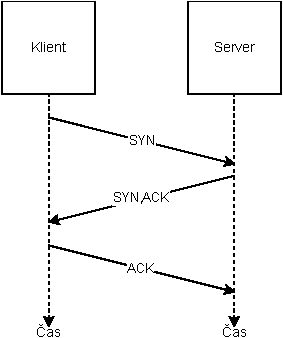
\includegraphics[width=0.33\textwidth]{obrazky-figures/3way-handshake-tcp.pdf}
	\caption{Handshake TCP}
	\label{fig:tcp-handshake}
\end{wrapfigure}
\FloatBarrier

TCP je nejpoužívanějším protokolem \textit{transportní vrstvy} v~sadě protokolů \textit{TCP/IP}, poskytuje spolehlivou službu přenosu dat po~bytech pro~aplikace. Aplikační přenos dat po~bytech je přenášen přes síť prostřednictvím TCP segmentů, přičemž každý TCP segment je odeslán jako datagram protokolu IP (Internet Protocol). Spolehlivost TCP spočívá v~detekci ztráty segmentů (pomocí pořadových čísel) a~chyb (pomocí kontrolních součtů pro~každý segment) a~také v~jejich opravě prostřednictvím opětovného přenosu~\cite{rfc-tcp}. Předtím, než jeden proces může začít posílat data druhému, musí se nejdříve oba vzájemně \uv{domluvit}, tedy provedou takzvaný \textit{handshake}~\cite{kurose2021}. To znamená, že si musí vyměnit několik úvodních segmentů, aby stanovily parametry následného přenosu dat. Handshake obsahuje přesně 3 segmenty. První dva nenesou žádnou zátěž, tedy žádná data aplikační vrstvy, třetí segment ji nést může. Z~počtu segmentů při~ustanovení spojení také vyplývá název \uv{three-way handshake} (\uv{třífázové navázáni spojení} – nadále bude využívána anglická forma, jelikož je to běžné i~mezi~odborníky v~oboru), jak je znázorněno v~diagramu~\ref{fig:tcp-handshake}. Při~komunikaci se pro~ověření správného pořadí segmentů a~případné vyžádání opětovného zaslání ztraceného segmentu používají \textit{sekvenční} (sequence) a~\textit{potvrzovací} (acknowledgment) čísla. Tyto čísla se rovněž používají ve~fázi \textit{three-way handshake}.
\newpage
Navázání spojení probíhá následovně:
\begin{enumerate}
	\item Klient odešle na~server datagram s~příznakem \textit{SYN}\footnote{Synchronize sequence number (česky synchronizace pořadového čísla)}, náhodně vygenerovaným pořadovým číslem $X$ a~potvrzovacím číslem 0.
	\item Server odešle klientovi datagram s~příznaky \textit{SYN} a~\textit{ACK}\footnote{Acknowledgment (česky potvrzení)}, potvrzovacím číslem $X+1$ a~náhodně vygenerovaným pořadovým číslem $Y$. 
	\item Klient dokončuje navázání datagramem s~příznakem \textit{ACK}, pořadovým číslem $X+1$ a~potvrzovacím číslem odpovědi $Y+1$.
\end{enumerate}
Jak již bylo zmíněno, TCP je jedním z~nejpoužívanějších spolehlivých protokolů v~dnešní době. Zajišťuje spolehlivé doručování dat mezi~dvěma koncovými body, avšak má také své neduhy. Jedním z~nejvýraznějších je absence jakéhokoli šifrování, což znamená, že veškerá data přenášená pomocí TCP jsou odesílána v~otevřené, nešifrované podobě. Tato slabina může být využita k~odposlechu nebo manipulaci s~daty, což představuje bezpečnostní riziko. 

Na řadu tedy přichází \textit{TLS} protokol, který poskytuje \textit{šifrování} a~\textit{autenticitu} na~transportní vrstvě\footnote{TLS nelze přesně zařadit k~jedné vrstvě ISO/OSI modelu}, a~tím umožňuje bezpečný přenos aplikačních dat. V~následující podkapitole~\ref{sec:tls} jsou blíže popsány principy fungování a~využití \textit{TLS} v~kombinaci s~\textit{TCP}.

\section{Transport Layer Security – TLS}
\label{sec:tls}
Šifrování, autentizace a~integrita jsou tři zásadní bezpečnostní funkce, které \textit{TCP} postrádá a~\textit{TLS} naopak poskytuje. Tento protokol je nástupcem \textit{SSL}\footnote{Secure Sockets Layer (vrstva bezpečných schránek)}, který byl nahrazen kvůli závažným bezpečnostním chybám a~nedostatečné odolnosti vůči útokům. \textit{TLS} nabízí modernější šifrovací algoritmy a~lepší zabezpečení, čímž překonává nedostatky \textit{SSL}. V~dnešní době je \textit{SSL} prakticky historií, a~proto se tato práce zaměřuje výhradně na~komunikaci pomocí \textit{TLS}. Vzhledem k~tomu, že v~poskytnutých datových sadách, jak je zmíněno v~sekci~\ref{sec:dataset}, se převážně objevuje \textit{TLS} \textbf{verze 1.2}, bude pozornost této sekce věnována právě této verzi.

Protokol se skládá ze dvou vrstev: \textit{TLS Record Protocol} a~\textit{TLS Handshake Protocol}. \textit{Record Protokol} zapouzdřuje různé protokoly vyšších vrstev. Jeden z~těchto zapouzdřených protokolů je \textit{TLS Handshake}, který umožňuje serveru a~klientovi vzájemnou autentizaci a~vyjednání šifrovacích algoritmů a~kryptografických klíčů před~zahájením komunikace aplikačních protokolů.

\textit{TLS Record Protocol} následně přebírá data aplikační vrstvy, která mají být přenesena. Operuje nad~těmito daty, která jsou nejprve fragmentována, případně komprimována, je k~nim přidán kód MAC (Message Authentication Code\,--\,kód autentizace zprávy), poté jsou zašifrována a~přidána hlavička protokolu. Takto vytvořená datová jednotka je poté předána do~TCP segmentu pro~přenos~\cite{Stallings2017}.


Jednou z~výhod je skutečnost, že \textit{TLS} je nezávislý na~aplikačním protokolu a~datech aplikační úrovně, které šifruje. Protokoly vyšší úrovně mohou na~něj navazovat \textbf{transparentně}. Kromě snad nejpoužívanějšího aplikačního protokolu HTTP se TLS využívá také pro~protokoly jako například \textit{FTP}, \textit{SMTP}, \textit{NNTP} a~další. TLS není omezeno pouze na~funkčnost nad~TCP, ale dokáže zabezpečit komunikaci stejně přes \textit{UDP} či \textit{DCCP}. Díky již zmíněné transparentnosti vůči přenášenému aplikačnímu protokolu může také poskytovat zabezpečení při~VPN spojení, typicky v~případě použití \textit{OpenConnect} nebo \textit{OpenVPN}~\cite{rfc-sec_proto}. Další možností využití je při~e-mailové komunikaci pomocí příkazu \textit{STARTTLS}~\cite{matousek2014}.

Standard však nespecifikuje, jak protokoly implementují zabezpečení pomocí \textit{TLS}. Rozhodnutí o~tom, jak zahájit \textit{handshake} a~jak interpretovat autentizační certifikáty, které jsou vyměněny, jsou ponechána na~uvážení návrhářů a~vývojářů protokolů operujících nad~\textit{TLS}~\cite{rfc-tls12}. 

Dle \textit{ISO/OSI} modelu nelze protokol \textit{TLS} správně klasifikovat, jelikož operuje především nad~\textit{TCP}, které se nachází ve~4. vrstvě, a~samotné \textit{TLS} poskytuje bezpečné navázání a~udržení relace, při~fázi \textit{handshake}, což je funkce 5. vrstvy (\textit{relační}). Zároveň šifruje aplikační data, což je funkcí prezentační vrstvy. Z~pohledu šifrování, které je hlavní funkcí, lze \textit{TLS} nejlépe zařadit do~6. vrstvy (\textit{prezentační}). Nicméně klasifikace \textit{TLS} pouze do~jedné vrstvy není přesná, protože plní funkce napříč několika vrstvami modelu \textit{ISO/OSI}.

\subsection{Základní bezpečnostní funkce}

Tato podkapitola, převzata a~upravena z~\cite{rfc-tls12}, se zaměřuje na~základní bezpečnostní funkce protokolu TLS, konkrétně na~symetrickou kryptografii, integritu dat a~autentizaci, které společně zajišťují bezpečnost komunikace.

\subsubsection{Důvěrnost}
Symetrická kryptografie je základní metodou pro~šifrování přenášených dat. Pro~šifrování se používají různé algoritmy, jako je \textit{AES} (Advanced Encryption Standard), který je v~dnešní době považován za~velmi bezpečný a~široce používaný. Starší algoritmy, jako \textit{RC4}, byly dříve běžně nasazovány, ale kvůli nalezeným zranitelnostem a~slabinám jsou již považovány za~zastaralé a~jejich použití se nedoporučuje~\cite{rfc-rc4}.

Důvěrnost je zajištěna tím, že klíče používané pro~šifrování jsou unikátně generovány pro~každou relaci (tzv.~\uv{session}). Tyto klíče se odvozují z~tajemství, které je bezpečně vyjednáno během \textit{handshake} fáze. Nejběžněji používanými metodami jsou výměny klíčů na~bázi algoritmů \textit{Diffie-Hellman} a~\textit{RSA}, který se používá pro~asymetrické šifrování. Protokol \textit{TLS} rovněž umožňuje komunikaci bez~šifrování, což však odporuje hlavnímu účelu protokolu.

\subsubsection{Integrita dat}
Kontrola integrity je klíčová pro~zajištění, že data nebyla během přenosu pozměněna třetí stranou. Přenos zpráv zahrnuje kontrolu integrity zpráv pomocí hodnoty \textit{MAC}. Pro~výpočet MAC se používají bezpečné hašovací algoritmy, jako je \textit{SHA-256}, který se stal standardem pro~moderní aplikace. Starší algoritmy, jako je \textit{MD5} a~\textit{SHA-1}, byly dříve široce používány, ale kvůli objevení kolizí a~zranitelností se již nedoporučují~\cite{sha-collision}.

\subsubsection{Autentizace}
Autentizace se nejčastěji provádí pomocí asymetrické kryptografie. Servery se autentizují vůči klientům pomocí digitálních certifikátů, které obsahují veřejný klíč serveru a~jsou podepsány důvěryhodnou certifikační autoritou (CA). Autentizace klientů je volitelná, ale v~některých případech, například v~případě přístupu k~citlivým systémům, může být požadována. Nejčastěji se používají algoritmy jako \textit{RSA} nebo \textit{ECDSA}.

Tyto základní bezpečnostní funkce symetrické kryptografie, integrity dat a~autenticity společně zajišťují důvěryhodnost a~bezpečnost moderní internetové komunikace, čímž umožňují uživatelům důvěřovat přenášeným informacím.

\subsection{Navázání spojení}

Počátkem každé komunikace je navázání spojení mezi~účastníky. U~TLS tomu není jinak a, jak již bylo zmíněno, tato fáze se nazývá \uv{TLS handshake}. Po~navázání a~ustanovení spojení protokolem \textit{TCP}, k~čemuž slouží \textit{three-way handshake}, jenž je podrobně rozepsán v~\ref{sec:tcp}, se \textit{TLS} pokusí navázat bezpečné spojení a~vyjednat detaily budoucí komunikace. Pro~lepší představu je znázorněno diagramem~\ref{fig:tls-handshake}.

\begin{wrapfigure}{R}{0.33\textwidth}
	\centering
	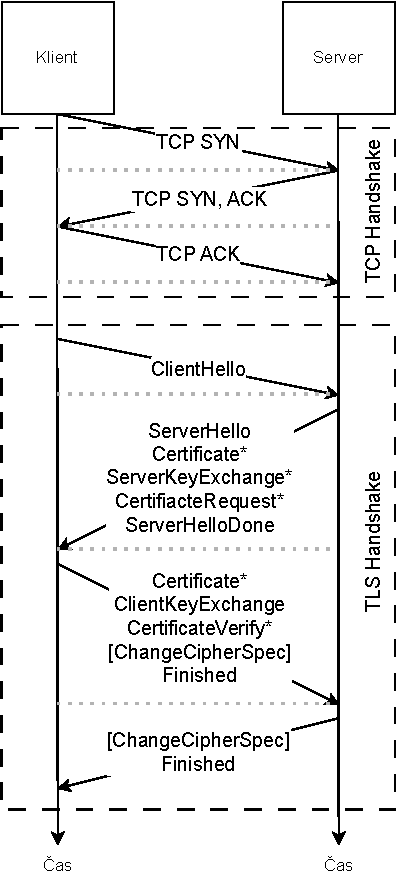
\includegraphics[width=0.33\textwidth]{obrazky-figures/tls-handshake.pdf}
	\caption{Handshake TLS}
	\label{fig:tls-handshake}
\end{wrapfigure}
\FloatBarrier

Postup ustanovení spojení mezi~klientem a~serverem probíhá následovně:
\begin{enumerate}
	\item Klient zašle zprávu \textit{ClientHello}, obsahující seznam kryptografických algoritmů, které podporuje, spolu s~náhodně vygenerovaným číslem (označovaným jako \uv{nonce}\footnote{Kryptografická nonce je označení pro~náhodné číslo, které lze použít pouze jednou. Jeho přítomnost zvyšuje obtížnost podvržení zprávy.}).
	\item Ze seznamu je serverem vybrán algoritmus pro~\textbf{symetrickou} kryptografii, algoritmus pro~\textbf{asymetrickou} kryptografii a~typ \textbf{\textit{HMAC}} (Hash-based Message Authentication Code, česky autentizační kód zprávy). Dále je zvolena \textbf{hašovací funkce}, např. \textit{MD5}, \textit{SHA-2},\dots Vybrané algoritmy jsou zaslány zpět klientovi spolu s~certifikátem serveru a~náhodně vygenerovaným číslem (nonce), jako součást zprávy \textit{Server Hello}.
	\item Klient ověří certifikát, získá veřejný klíč serveru, vygeneruje \textit{Pre-Master Secret} (dále označovaný jako \uv{PMS}), zašifruje \textit{PMS} veřejným klíčem serveru a~odešle šifrovaný \textit{PMS} serveru.
	\item Pomocí stejné funkce pro~odvození klíče, jak je stanoveno standardem \textit{TLS}~\cite{rfc-tls12}, klient a~server nezávisle vypočítají \textit{Master Secret} (dále označovaný jako \uv{MS}) z~\textit{PMS} a~nonce. \textit{MS} se poté rozdělí na~dva šifrovací klíče a~dva \textit{HMAC} klíče. Dále, pokud vybraný symetrický šifrovací algoritmus používá režim \textit{CBC} (Cipher Block Chaining, česky \uv{Řetězení šifrovacích bloků}, a~dále označován zkratkou \textit{CBC}), například \textit{3DES} nebo \textit{AES}, jsou z~\textit{MS} získány také dva inicializační vektory (\textit{IV}) --jeden pro~každou stranu spojení. Následně jsou všechny zprávy mezi~klientem a~serverem šifrovány a~autentizovány (pomocí \textit{HMAC}). Obě strany si vzájemně zašlou \textit{HMAC} vypočítaný na~základě všech předchozích zpráv, aby ověřily integritu celé fáze navazování a~vyjednávání spojení.
\end{enumerate}

Proces navazování spojení, odehrávající se v~5.vrstvě (\textit{relační}) \textit{ISO/OSI} modelu, pomocí protokolu \textit{TLS Handshake} je klíčovým prvkem k~zajištění bezpečné komunikace mezi~dvěma stranami. Správný výběr algoritmů a~hašovacích funkcí, ověřování HMAC a~použití nonce jsou zásadní pro~ochranu dat a~zajištění důvěrnosti. V~další podsekci~\ref{sec:clienthello} je podrobně popsán obsah těchto zpráv, které nejsou šifrovány a~využívají se k~tvorbě TLS otisku. Bližší popis TLS otisku je v~kapitole~\ref{chp:JA34}.

\subsection{Obsah zprávy Client Hello}
\label{sec:clienthello}
V této podsekci je popsán obsah zpráv \textit{Client Hello}. Následující struktura\textit{Client Hello} zpráv je převzata z~\textbf{RFC 5246}~\cite{rfc-tls12}. 

Struktura \textit{Client Hello} je definována následovně:
\begin{verbatim}
struct 
{
    ProtocolVersion client_version;
    Random random;
    SessionID session_id;
    CipherSuite cipher_suites<2..2^16-2>;
    CompressionMethod compression_methods<1..2^8-1>;
    select (extensions_present) 
    {
        case false:
          struct {};
        case true:
          Extension extensions<0..2^16-1>;
    };
} ClientHello;
\end{verbatim}
Kde:
\begin{itemize}
	\item \textbf{client\_version} značí verzi \textit{TLS} protokolu, kterou klient podporuje (např. 771\,--\,pro \textit{TLS v1.2}),
	\item \textbf{random} je klientská nonce,
	\item \textbf{session\_id} označuje identifikátor relace,
	\item \textbf{cipher\_suites} reprezentuje seznam šifrovacích sad podporovaných klientem,
	\item \textbf{compression\_methods} značí seznam metod komprese podporovaných klientem,
	\item \textbf{extensions\_present} indikuje přítomnost rozšíření,
	\item \textbf{extensions}, je kolekce rozšíření poskytujících dodatečné zabezpečení spojení. Běžná rozšíření jsou například \textit{supported\_groups}, které identifikuje eliptické křivky podporované klientem, a~\textit{ec\_point\_formats}, které specifikuje množinu bodů používaných pro~reprezentaci eliptických křivek~\cite{rfc-tls-ext}. Více v~\ref{subsec:ext}.
\end{itemize} 

Zpráva \textit{Client Hello} je zásadním \uv{stavebním kamenem} \textit{TLS} komunikace, protože propaguje možnosti a~vlastnosti klienta, jako jsou podporované verze protokolu, šifrovací sady a~rozšíření. Hodnoty vybraných atributů zprávy  mohou být použity pro~identifikaci pomocí \textit{JA3/JA4} otisků, více viz~\ref{chp:JA34}.


\subsection{Obsah zprávy Server Hello}
\label{sec:serverhello}
Následující struktura \textit{Server Hello} zprávy je převzata z~\textbf{RFC 5246}~\cite{rfc-tls12}. Struktura zprávy \textit{Server Hello} je následující:

\begin{verbatim}
struct 
{
    ProtocolVersion server_version;
    Random random;
    SessionID session_id;
    CipherSuite cipher_suite;
    CompressionMethod compression_method;
    select (extensions_present) 
    {
        case false:
          struct {};
        case true:
          Extension extensions<0..2^16-1>;
    };
} ServerHello;
\end{verbatim}
Kde:
\begin{itemize}
	\item \textbf{server\_version} značí verzi \textit{TLS} protokolu, kterou server vybral na~základě \textit{client\_version},
	\item \textbf{random} je nonce serveru,
	\item \textbf{session\_id} označuje identifikátor relace,
	\item \textbf{cipher\_suite} reprezentuje jednu šifrovací sadu vybranou z~\textit{cipher\_suites},
	\item \textbf{compression\_method} značí jednu metodu komprese zvolenou serverem,    
	\item \textbf{extensions\_present} indikuje přítomnost rozšíření,
	\item \textbf{extensions}, stejně jako u~\textit{Client Hello}, určuje jaká rozšíření vybraná serverem jsou podporována. Více v~\ref{subsec:ext}.
\end{itemize}

Výběr z~výše zmíněných elementů zpráv je využit pro~tvorbu a~následnou identifikaci pomocí \textit{JA3/JA4} otisků, jak je detailněji popsáno dále v~kapitole~\ref{chp:JA34}. V~následující podsekci~\ref{sec:tls-13} jsou rozepsány podrobnosti implementace \textit{TLS} verze \textit{1.3} a~také jsou zmíněny změny \textit{Hello} zpráv oproti verzi \textit{1.2}. 

\subsection{Možná rozšíření}
\label{subsec:ext}
Detailní popis všech možných atributů a~funkcí těchto zpráv je nad~rámec této technické zprávy. Proto jsou uvedeny pouze potřebné informace pro~pochopení a~následné vysvětlení v~kontextu s~\textit{JA3} a~\textit{JA4} otisky. Z~tohoto důvodu jsou zde uvedena pouze nejčastější a~informačně nejvýznamnější rozšíření, která jsou používána k~tvorbě otisků nebo ke~zlepšení přesnosti identifikace.

\begin{itemize}
	\item \textbf{Server Name Indicator} (\textit{Indikátor jména serveru}, dále jen \uv{SNI}) umožňuje klientům poskytnout název serveru, se kterým se spojují. Tato funkce je žádoucí pro~usnadnění zabezpečených připojení k~serverům, které provozují více \uv{virtuálních} serverů na~jedné adrese~\cite{rfc-sni}.
	      	          
	\item \textbf{Application-Layer Protocol Negotiation} (\textit{Vyjednání aplikačního protokolu}, dále jen \uv{ALPN}) V~situaci, kdy je na~jednom portu serveru, například portu 443, podporováno více aplikačních protokolů, klient a~server musí vyjednat aplikační protokol, který bude použit pro~každé připojení. S~\textit{ALPN} klient odesílá seznam podporovaných aplikačních protokolů jako součást zprávy \textit{TLS Client Hello}. Server si vybere protokol a~odešle vybraný protokol jako součást zprávy \textit{TLS Server Hello}~\cite{rfc-alpn}. Vyjednávání aplikačního protokolu tak může být provedeno v~rámci protokolu \textit{handshake}, aniž by se přidávaly další síťové výměny, a~umožňuje serveru přiřadit k~jednotlivým aplikačním protokolům různé certifikáty.
	      	      
\end{itemize}

\subsection{TLS verze 1.3}
\label{sec:tls-13}
\textit{TLS verze 1.3} je \textbf{nejnovější} verzí protokolu \textit{TLS}. Mezi~nejvýznamnější rozdíly posledních dvou verzí patří především změny v~seznamu povolených šifer u~symetrické kryptografie, kde v~novější verzi zůstávají pouze \textbf{AEAD} (\textit{Authenticated Encryption with Associated Data} -- česky autentizované šifrování s~připojenými daty) algoritmy. \textit{Handshake} protokol je zrychlen pomocí techniky \textbf{0-RTT} (\textit{Zero Round-Trip Time} -- česky nulová doba navázání spojení), která šetří jednu cestu tam a~zpátky na~úkor některých bezpečnostních vlastností. Nová verze také \textbf{šifruje} všechny zprávy protokolu \textit{Handshake} po~zprávě \textit{Server Hello}~\cite{rfc-tls13}. Plánuje se také začít šifrovat \textit{Hello} zprávy, čímž se znemožní identifikaci pomocí pouhých \textit{JA3}/\textit{JA4} otisků~\cite{encrypted-hello}.

Také byly představeny takzvané \textbf{GREASE} (\textit{Generate Random Extensions And Sustain Extensibility}) hodnoty, které jsou přidávány do~atributů zpráv handshake protokolu, k~ověření správné implementace protější strany. Při~správném zpracování musí být tyto hodnoty ignorovány druhou stranou. V~případě, že \textit{GREASE} hodnoty nejsou tolerovány, je vyhlášena chyba, která značí nevalidní implementaci~\cite{rfc-grease}.

\textit{TLS} je typicky implementován nad~\textit{TCP} protokolem, ovšem verze 1.3 dokáže komunikovat také přes \textit{UDP} (\textit{User Datagram Protocol}) v~případě, že je použit protokolem \textbf{QUIC} (\textit{Quick UDP Internet Connections}). \textit{QUIC} využívá \textit{UDP} jako transportní protokol a~zároveň na~něm staví pokročilé funkce, jako je správa spojení a~zajištění spolehlivosti~\cite{rfc-quic}. Má zabudované zabezpečení pomocí \textit{TLS v1.3}, díky čemuž poskytuje všechny bezpečnostní výhody \textit{TLS}~\cite{rfc-quic-tls}.

    \chapter{Otisky JA3, JA4 a~jejich použití}
\label{chp:JA34}
Tato kapitola se zabývá pasivními metodami pro~identifikaci šifrované komunikace a~jejich vývojem od~\textit{JA3} k~\textit{JA4+}. 
S narůstajícím trendem šifrování v~síťovém provozu bylo třeba vyvinout způsob klasifikace či identifikace šifrovaných dat kvůli správě a~analýze komunikace. V~roce 2015 byla představena, dnes již populární až možná zastaralou, pasivní metodu tvorby otisků TLS spojení označovanou jako \textit{JA3} otisky\footnote{Více na~\url{https://github.com/salesforce/ja3}}. Tvůrci \textit{John~B.~Althouse}, \textit{Jeff~Atkinson} a~\textit{Josh~Atkins} v~rámci společnosti \textit{Salesforce} ve~své metodě využívají atributy \textit{Hello} zpráv \textit{TLS} spojení. S~příchodem nové verze \textit{TLS v1.3}, která šifruje všechny zprávy protokolu \textit{Handshake} po~odeslání \textit{Server Hello} a~umožňuje využívat jako transportní protokol \textit{QUIC}, stejně jako další změny, které ztěžují efektivní identifikaci, již nebylo možné aplikovat \textit{JA3} otisky pro~tato spojení.

Pro pasivní metody identifikace zabezpečené komunikace se tak objevuje další výzva. V~roce 2023 přichází na~řadu sada metod \textit{JA4+}\footnote{Více na~\url{https://github.com/FoxIO-LLC/ja4}}, od~stejných tvůrců, v~zastoupení firmy \textit{FoxIO}. Příklady využití těchto otisků zahrnují skenování pro~odhalení hrozeb, detekci malwaru, prevenci únosu relace, automatizaci dodržování předpisů, sledování polohy, detekci \textit{DDoS} útoků, seskupování hrozeb, detekci reverzních shellů a~mnoho dalších~\cite{Althouse2023}.

V následující sekci~\ref{sec:JA3} je představen koncept \textit{JA3} otisků a~jejich využití. Na~ni navazuje sekce~\ref{sec:JA4+}, která seznamuje se sadou metod \textit{JA4+} pro~identifikaci různých vlastností šifrovaných spojení, jejichž součástí jsou také \textit{JA4} otisky. Porovnání \textit{JA3} a~\textit{JA4} otisků lze nalézt v~podsekci~\ref{sec:compJA34}.

\section{JA3 otisky}
\label{sec:JA3}
JA3 (pojmenování vzniklo podle jmen tří hlavních tvůrců: \textbf{J}ohn B. \textbf{A}lthouse, \textbf{J}eff \textbf{A}tkinson a~\textbf{J}osh \textbf{A}tkins) je metoda tvorby otisku \textit{TLS} spojení, která se zaměřuje na~různé aspekty a~atributy \textit{TLS handshake}. Používá hodnoty ze zpráv \textit{Client Hello} či \textit{Server Hello}, které obsahují několik detailů, jež dokážou jedinečně charakterizovat jak klienta, tak server. Po~extrakci těchto informací jsou jednotlivé hodnoty zřetězeny a~je proveden výpočet haše typu \textit{MD5}. Výstup hashovací funkce představuje zmíněný \textit{JA3} otisk, který poskytuje konzistentní a~identifikovatelný podpis.


Metoda \textit{JA3} využívá následující atributy \textit{Client Hello}: \texttt{client\_version}, \texttt{cipher\_suite}, \texttt{extensions}, \texttt{supported\_groups}\footnote{Dříve definováno jako \texttt{elliptic\_curves}} a~\texttt{ec\_point\_formats}\footnote{Dříve definováno jako \texttt{elliptic\_curve\_point\_formats}}. Pro~podrobnější popis těchto polí zprávy viz.~sekce~\ref{sec:clienthello}. Tyto hodnoty jsou pak spojeny dohromady v~uvedeném pořadí, přičemž jednotlivá pole jsou oddělena čárkou (`,`) a~hodnoty v~rámci každého pole jsou odděleny pomlčkou (`--`). Musí být brány v~potaz také hodnoty \textit{GREASE}; bližší popis lze nalézt v~sekci~\ref{sec:tls-13}. Při~extrakci hodnot z~polí jsou buďto ignorovány, nebo nahrazeny konstantou, aby byla zachována konzistence otisku.

Pro lepší porozumění je předvedena názorná ukázka, převzata z~\cite{Althouse2022JA3}.
Řetězec po~zpracování všech výše zmíněných polí vypadá následovně. Tento řetězec je poté použit jako vstup do~hashovací funkce \textit{MD5}, která vytvoří daný otisk.
\begin{table}[H]
	\centering
	\begin{tabular}{c|c}
		Řetězec & \verb|769,47–53–5–10–49161–49162–49171–49172–50–56–19–4,0–10–11,23–24,0| \\
		          & $\downarrow$                                                                                         \\
		Otisk     & \verb|ada70206e40642a3e4461f35503241d5|                                                              \\ 
	\end{tabular}
\end{table}

V případě, že nejsou žádná rozšíření dostupná, pole jsou ponechána prázdná:
\begin{table}[H]
	\centering
	\begin{tabular}{c|c}
		Řetězec & \verb|769,4–5–10–9–100–98–3–6–19–18–99,,,| \\        
		          & $\downarrow$                                                   \\
		Otisk     & \verb|de350869b8c85de67a350c8d186f11e6|                        \\ 
	\end{tabular}
\end{table}

Tato metoda se dá také aplikovat na~zprávu \textit{Server Hello} pro~identifikaci serveru. Jedná se o~takzvaný \textit{JA3S} otisk. Využívá hodnoty polí \texttt{server\_version}, \texttt{cipher\_suite} a~\texttt{extensions}, jak je podrobněji popsáno v~sekci~\ref{sec:serverhello}. Postup je poté totožný s~tvorbou otisku pro~klienta, a~to tedy zřetězením a~použitím jako vstupu pro~hashovací funkci \textit{MD5}.

Ukázka tvorby \textit{JA3S} otisku, také převzata z~\cite{Althouse2022JA3}:
\begin{table}[H]
	\centering
	\begin{tabular}{c|c}
		Řetězec & \verb|769,47,65281–0–11–35–5–16| \\        
		          & $\downarrow$                               \\
		Otisk     & \verb|4835b19f14997673071435cb321f5445|    \\ 
	\end{tabular}
\end{table}

V průběhu času se však ukázalo, že \textit{JA3} otisky již nejsou tak přesné, jak bylo potřeba, a~to z~následujících důvodů:
\begin{itemize}
	\item \textbf{Náhodné uspořádání TLS rozšíření}: Některé prohlížeče začaly náhodně měnit pořadí rozšíření za~účelem zmaření snah o~identifikaci. \textit{JA3} otisky se spoléhají na~sekvenční pořadí, které se náhodným řazením mění, což mělo za~důsledek \textbf{nespolehlivost} při~identifikaci jedinečných klientů.
	\item \textbf{Nekonzistence databází}: Implementace tvorby se lišily pro~různé programy a~databáze, což vedlo \textbf{k různým výsledkům pro~stejnou identifikovanou entitu}. Tato nejednotnost bránila efektivnímu a~spolehlivému sdílení otisků.
	\item \textbf{Omezený rozsah}: \textit{JA3} se zaměřovaly pouze na~prvky v~rámci \textit{Hello} zpráv \textit{TLS} spojení. Tento omezený rozsah často postrádal kontext o~prostředí klienta. Navíc, s~rostoucí popularitou novějších transportních protokolů, jako například \textit{QUIC}, se ukázalo, že \textbf{identifikace je neúčinná}.
\end{itemize}

\subsection{Spolehlivost a~omezení JA3 otisků}
Mobilních aplikací pomocí \textit{TLS} otisků lze považovat za~praktickou metodu s~potenciálním využitím v~digitální forenzní analýze. Studie ukázaly, že samotné použití \textit{JA3} otisku není pro~přesnou identifikaci mobilních aplikací dostačující. Spolehlivějších výsledků je dosaženo kombinací \textit{JA3}, \textit{JA3S} a~\textit{SNI}, přičemž všechny tyto charakteristiky lze jednoduše získat z~\textit{TLS} handshake zpráv~\cite{MatousekMobileDevice2020}. Rovněž byla zkoumána volatilita \textit{TLS} otisků \,--\, experimenty ukázaly, že jejich variabilita není výrazná~\cite{MatousekJA3Reliability2020}.

\subsection{Shrnutí a~přechod na~JA4+}
\textit{JA3} otisky poskytují jednoduchou a~rychlou identifikaci \textit{TLS} spojení; ovšem s~příchodem nové verze \textit{TLS 1.3} se stávají zastaralými a~jejich přesnost klesá. Řešením je využít jiné metody klasifikace nebo použít nového nástupce těchto otisků. V~následující sekci~\ref{sec:JA4+} je probírána sada metod \textit{JA4+}, která slouží jako novější verze \textit{JA3} a~přináší s~sebou také další možnosti analýzy, a~to nejen \textit{TLS} spojení.

\section{Sada metod JA4+}
\label{sec:JA4+}
Kvůli již zmíněným důvodům, které vedly k~nepřesnosti identifikace, byl vyvinut nástupce \textit{JA3} otisků, a~to \textit{JA4}. Přesněji se jedná o~sadu metod \textit{JA4+}, které dokáží identifikovat i~jinou komunikaci než pouze \textit{TLS}. V~této sadě se nachází jak metody \textit{JA4} a~\textit{JA4S} pro~tvorbu otisků \textit{TLS}, tak například \textit{JA4HTTP}, \textit{JA4Latency}, \textit{JA4SSH}, \textit{JA4TCP} a~další\dots V~rámci této práce je pozornost zaměřena pouze na~metody \textbf{JA4} a~\textbf{JA4S}.

\subsection{Metoda JA4}
\textit{JA4} přistupuje k~identifikaci podobně jako metoda JA3. Využívá určité hodnoty z~polí \textit{Hello} zpráv, které buď zřetězí, nebo z~nich vypočítá hash pomocí hashovací funkce \textit{SHA256}. Formát otisku je rozdělen do~tří částí (a, b, c), oddělených podtržítkem (\_). Každou z~těchto částí lze označit, což zjednodušuje použití v~situacích, kdy je k~identifikaci potřeba pouze konkrétní část~\cite{Althouse2023}. 

\subsection{Formát otisku JA4}
Tato podsekce se zaměřuje na~formát otisku \textit{JA4}. Na~základě uvedených příkladů lze vidět, jak je otisk strukturován a~z~jakých částí se skládá. Příklady formátu otisku jsou převzaty z~\cite{Althouse2023}. Formát otisku \textit{JA4} je následující:
\[
	\text{JA4} = \text{JA4a} \_ \text{JA4b} \_ \text{JA4c}
\]

Kde:
\begin{itemize}
	\item \textbf{JA4a} představuje konkatenaci vybraných informací o~TLS spojení, jako je:
	      \begin{itemize}
	      	\item Protokol, označený jako \texttt{\uv{t}} (\textit{TCP}) nebo \texttt{\uv{q}} (\textit{QUIC}),
	      	\item Verze TLS: 1.2 = \texttt{\uv{12}}, 1.3 = \texttt{\uv{13}},
	      	\item SNI, \texttt{\uv{d}} pro~doménu nebo \texttt{\uv{i}} pro~\textit{IP} adresu,
	      	\item Počet šifrovacích sad,
	      	\item Počet rozšíření,
	      	\item První hodnota \textit{ALPN}.
	      \end{itemize}
	      	      
	\item \textbf{JA4b} je zkrácený hash (12B) (\textit{SHA-256}) nad~seřazeným seznamem šifrovacích sad.
	      	      
	\item \textbf{JA4c} je také zkrácený hash (12B) (\textit{SHA-256}) nad~seřazeným seznamem rozšíření a~algoritmů pro~podpisy (\textit{signature algorithms}) v~pořadí, ve~kterém se objevují.
	      	      
\end{itemize}
Konkrétní příklad může vypadat takto:
\[
	\text{JA4} = \texttt{t13d1516h2} \_ \texttt{acb858a92679} \_ \texttt{e5627efa2ab1}
\]
	      
	      
Podobně jako u~svého předchůdce \textit{JA3}, umožňuje sada \textit{JA4} identifikaci serverové strany \textit{TLS} komunikace prostřednictvím analýzy zprávy \textit{Server Hello}. Tato zpráva, odesílaná v~nezašifrované formě, reflektuje volbu serveru na~základě parametrů uvedených v~předchozí zprávě \textit{Client Hello}. Obsahuje mimo jiné jednu šifrovací sadu vybranou ze seznamu nabízeného klientem a~sadu rozšíření, které server zvolil pro~navázání spojení. Formát otisku \textbf{JA4S} je obdobný:

\[
	\begin{aligned}
		\text{JA4S} & = \text{JA4Sa} \_ \text{JA4Sb} \_ \text{JA4Sc} 
	\end{aligned}
\]

Kde:
\begin{itemize}
	\item \textbf{JA4Sa} obsahuje následující vybrané hodnoty:
	      \begin{itemize}
	      	\item Protokol, označený jako \texttt{\uv{t}} (\textit{TCP}) nebo \texttt{\uv{q}} (\textit{QUIC}),
	      	\item Verze TLS: 1.2 = \texttt{\uv{12}}, 1.3 = \texttt{\uv{13}},
	      	\item Počet rozšíření,
	      	\item První hodnota \textit{ALPN}.
	      \end{itemize}
	      	      
	\item \textbf{JA4Sb} představuje zvolenou šifrovací sadu (\textit{cipher suite}).
	      	      
	\item \textbf{JA4Sc} je zkrácený hash (\textit{SHA-256}) nad~seřazeným seznamem rozšíření.
\end{itemize}

Konkrétní příklad může vypadat takto:
\[
	\begin{aligned}
		\text{JA4S} & = \text{t1204000} \_ \text{c030} \_ \text{4e8089b08790} 
	\end{aligned}
\]

\subsection{Využití otisků JA4}
Použitelnost \textit{JA4} otisku je různorodá. Přesná identifikace jednotlivých aplikací je stále obtížná. Otisk však dokáže poskytnout množinu možných kandidátů, přičemž mohutnost této množiny může být poměrně vysoká. I~přesto tato informace napomáhá přesnější klasifikaci~\cite{BurgetovaJA42024}. \textit{JA4} lze také využít pro~identifikaci škodlivých aplikací (\textit{malwaru}) v~síťovém provozu. Ukazuje se, že za~použití dalších informací o~TLS spojení, jako je kombinace \textit{JA4}, \textit{JA4S} a~\textit{SNI}, se přesnost detekce zlepšuje~\cite{MatousekJA4Malware2024}.

\section{Srovnání otisků JA3 a~JA4}
\label{sec:compJA34}
Pro účely porovnání je níže uveden zkrácený výpis z~\textit{TLS} spojení se zvýrazněním prvků, které jsou využívány v~otiscích \textit{JA3} a~\textit{JA4}. (Položka \texttt{Extensions} reprezentuje ostatní rozšíření, která nejsou jmenovitě využita ani v~jedné z~verzí \textit{JA} otisků.)

\paragraph{Legenda}
\begin{itemize}
	\item \colorbox{ForestGreen!30}{JA3} – prvek použitý pouze v~otisku JA3
	\item \colorbox{DodgerBlue!30}{JA4} – prvek použitý pouze v~otisku JA4
	\item \colorbox{Plum!30}{JA3 + JA4} – prvek společný pro~oba otisky
\end{itemize}

\begin{TLSDisplay}
	Transport Protocol : \colorbox{DodgerBlue!30}{TCP}
	Handshake Type: Client Hello (1)
	Version: \colorbox{Plum!30}{TLS 1.2} (0x0303)
	Cipher Suites Length: \colorbox{DodgerBlue!30}{34}
	\colorbox{Plum!30}{Cipher Suites} \colorbox{DodgerBlue!30}{(17 suites)}
	Compression Methods Length: 1
	Compression Methods (1 method)
	Extensions Length: \colorbox{DodgerBlue!30}{560}
	Extension: \colorbox{DodgerBlue!30}{server_name name=tasks-pa.clients6.google.com}
	Extension: \colorbox{ForestGreen!30}{elliptic_curves} (len=2)
	Extension: \colorbox{ForestGreen!30}{ec_point_formats} (len=2)
	Extension: \colorbox{DodgerBlue!30}{application_layer_protocol_negotiation} (len=14)
	Extension: \colorbox{DodgerBlue!30}{signature_algorithms} (len=24)
	\dots
	\colorbox{Plum!30}{Extensions\dots}
\end{TLSDisplay}


Jak je patrné, otisky \textit{JA4} využívají širší spektrum informací, například transportní protokol nebo konkrétní rozšíření \textit{TLS}, což vede k~jejich vyšší unikátnosti a~spolehlivější identifikaci klientů~\cite{Althouse2023}.  Rozdíl je také v~tom, jak se s~těmito atributy nakládá. Starší verze \textit{JA3} odebere tzv.~\textit{GREASE} hodnoty, spojí je v~daném pořadí, přičemž používá znak \uv{,} k~oddělení jednotlivých polí a~znak \uv{-} k~oddělení hodnot v~každém poli. Tento řetězec je poté vstupem pro~hashovací funkci \textit{MD5}~\cite{Althouse2022JA3}. Jak lze spatřit v~diagramu~\ref{fig:JA3-creation}, jednotlivé kroky tohoto procesu jsou znázorněny sekvenčně.

\begin{figure}[H]
	\centering
	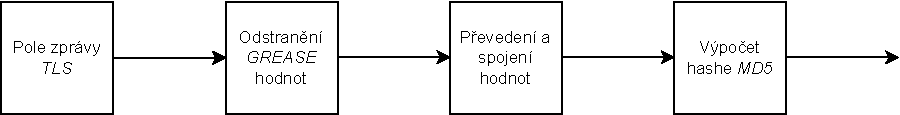
\includegraphics[width=\textwidth]{obrazky-figures/ja3-creation.drawio-crop.pdf}
	\caption{Proces tvorby otisků \textit{JA3}}
	\label{fig:JA3-creation}
\end{figure}
Novější verze \textit{JA4} vytváří otisky komplexnějším způsobem. První část otisku obsahuje zkonkatenizované hodnoty, druhá a~třetí část obsahují zkrácený hash \textit{SHA-256} nad~vybranými poli zprávy (seřazenými seznamy). Bližší popis je uveden v~sekci~\ref{sec:JA4+} nebo znázorněn diagramem~\ref{fig:JA4-creation}

\begin{figure}[H]
	\centering
	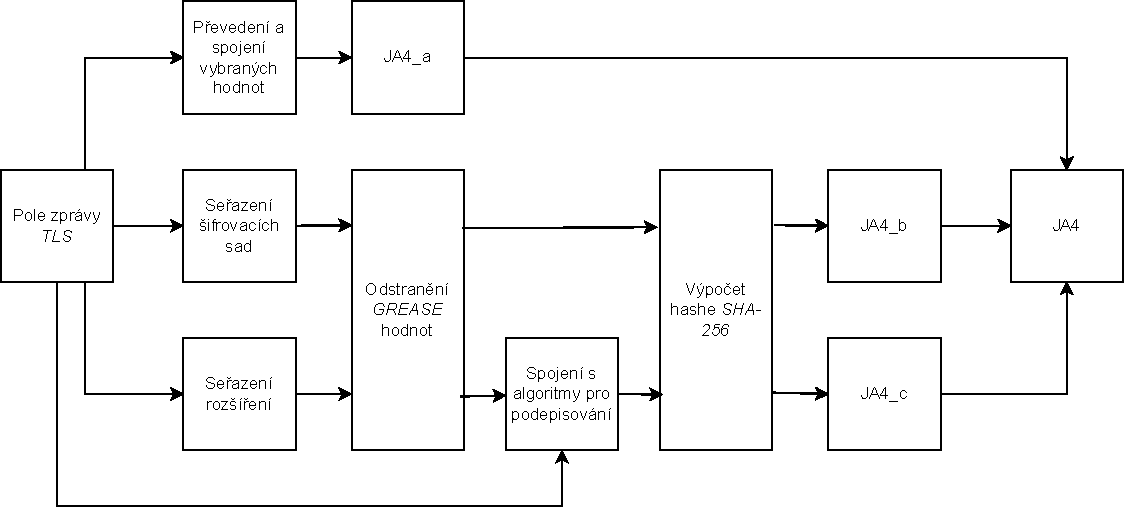
\includegraphics[width=\textwidth]{obrazky-figures/ja4-creation.drawio-crop.pdf}
	\caption{Proces tvorby otisků \textit{JA4}}
	\label{fig:JA4-creation}
\end{figure}

Z technického hlediska představuje sada metod \textit{JA4+} významný posun oproti svému předchůdci. Zatímco \textit{JA3} představuje jednoduchý a~stále využívaný nástroj, zaměřuje se pouze na~omezenou množinu atributů TLS zpráv. Naproti tomu \textit{JA4} zohledňuje širší spektrum informací, čímž zvyšuje unikátnost výsledného otisku.

Navíc \textit{JA4} implementuje vícefázový proces tvorby otisku – první část je tvořena explicitními hodnotami, následují hashované části, které zároveň eliminují vliv náhodného přehazování rozšíření a~šifrovacích sad. Použití \textit{SHA-256} namísto \textit{MD5} zvyšuje odolnost vůči kolizím.

Díky těmto změnám poskytuje \textit{JA4} výrazně přesnější identifikaci a~vyšší robustnost vůči technikám obfuskace, což z~něj činí užitečný nástroj pro~moderní síťovou analýzu.

    \chapter{Teoretické základy použitých algoritmů}
\label{chp: algos}
Za účelem zvýšení přesnosti identifikace aplikací, a~tedy zúžení kandidátní množiny generované pomocí metod \textit{JA3} či \textit{JA4}, je využit algoritmus pro~vyhledávání frekventovaných vzorů těchto otisků v~kontextu okolních \textit{TLS} spojení. Tato kapitola obsahuje obecný přehled algoritmů pro~vyhledávání frekventovaných vzorů, se zvláštním zaměřením na~princip a~využití algoritmu \textit{Apriori} a~jeho optimalizace.

Důvodem volby algoritmu \textit{Apriori} je jeho schopnost efektivně nacházet časté vzory v~transakčních datech, což lze analogicky aplikovat na~otisky \textit{TLS} spojení. Tento přístup umožňuje identifikovat opakující se kombinace otisků, které jsou charakteristické pro~specifické aplikace, a~tím efektivně eliminovat kandidáty, jejichž otisky s~těmito vzory nekorespondují.

\section{Algoritmy vyhledávající frekventované vzory}
Rozpoznávání frekventovaných vzorů v~datech představuje klíčovou a~nedílnou součást procesu dolování dat (\textit{data mining}). Tento krok umožňuje identifikovat opakující se vzory a~vztahy v~rozsáhlých datových souborech, které by jinak zůstaly skryté. V~rámci dolování dat se frekventované vzory využívají například pro~tvorbu asociačních pravidel, klasifikaci či shlukování. 

Typickými příklady využití jsou:
\begin{itemize}
	\item \textbf{Analýza nákupního chování zákazníků}, kde transakce představují množiny položek, které se společně vyskytují v~rámci nákupního chování~\cite{Aggarwal2014}.
	          
	\item \textbf{Analýza webových dat}, při~které se vyhledávají frekventované vzory ve~webových záznamech. Tyto vzory lze následně využít k~návrhu či vylepšení uživatelského rozhraní nebo ke~zlepšení personalizace obsahu~\cite{WebMining}. 
	          
	\item \textbf{Analýza softwarových chyb}, kde lze běh softwarových programů reprezentovat pomocí grafů obsahujících typické vzory. Logické chyby se často projevují jako specifické vzory, které je možné dále těžit pro~účely ladění a~diagnostiky~\cite{swBugs}.
\end{itemize}

Většina algoritmů pro~hledání frekventovaných vzorů je navržena v~rámci tradičního modelu založeného na~podpoře (\textit{support}) a~důvěře (\textit{confidence}). Existují však i~specializované přístupy, které využívají pokročilejší míry zajímavosti, modelují záporná pravidla nebo pracují s~omezeními pro~nalezení relevantnějších vzorů~\cite{Aggarwal2014}. Tato práce je zaměřena především na~algoritmus \textit{Apriori}, který je založen na~přístupu využívajícím podporu a~důvěru.

\section{Základní pojmy a~notace}
Před popisem samotného algoritmu \textit{Apriori} je vhodné uvést základní pojmy a~notace, které se v~oblasti dolování častých vzorů a~asociativních pravidel běžně používají.

\subsection{Transakce, položky a~jejich množiny}
Nechť množina položek \( I~= \{i_1, i_2, i_3, \dots, i_n\} \) reprezentuje například zboží v~obchodě či \textit{JA3/4} otisky \textit{TLS} spojení. Transakce \( T~\) je podmnožinou těchto položek, tedy \( T~\subseteq I~\). Množina všech transakcí tvoří transakční databázi \( D~= \{ T_1, T_2, T_3, \dots, T_m \} \). Množina položek (angl. \textit{itemset}) je libovolná kombinace prvků z~množiny \( I~\). Pokud množina položek (\textit{itemset}) obsahuje právě \( k~\) položek, nazýváme jej \textit{k-itemset}.

Množina častých položek (angl. \textit{frequent itemset}) je taková množina položek, která se v~transakční databázi vyskytuje alespoň s~minimální zadanou četností, zvanou podpora (\textit{support}). Míra \textit{podpory} (\textit{support}) je klíčovým kritériem pro~určení toho, zda je daná množina položek považována za~častou. 
Podpora množiny položek vyjadřuje, v~kolika transakcích z~celé databáze se daná množina vyskytuje. 
Formálně je definována jako:

\[
\text{support}(X) = \frac{\text{počet transakcí obsahujících } X}{\text{celkový počet transakcí}}
\]

Kandidátní množiny, jejichž podpora nedosahuje zvoleného prahu \textit{minsup} (minimální podpora), jsou z~dalšího zpracování vyřazeny.


\section{Algoritmus Apriori}
\textit{Apriori} je algoritmus určený pro~těžbu častých vzorců a~generování asociativních pravidel v~transakční databázích. Postupuje tak, že nejprve identifikuje časté jednotlivé položky v~databázi a~následně je rozšiřuje na~větší množiny, dokud se tyto množiny objevují v~databázi dostatečně často. Tyto časté vzory mohou být poté použity pro~generování asociativních pravidel, která reprezentují trendy a~závislosti v~databázi.

Algoritmus využívá přístup shora dolů pro~generování kandidátů, přičemž kandidáti jsou postupně rozšiřováni o~jednotlivé prvky. Skupiny kandidátů jsou následně ověřovány vůči databázi. Při~prohledávání se používá prohledávání do~šířky. Pro~efektivní počítání kandidátních množin je použita struktura hash stromu. Kandidátní množiny položek délky \(k\) se nejprve vytvoří na~základě množin častých položek délky \(k - 1\). Jsou odstraněny položky, které neobsahují podmnožinu s~častými položkami, a~prohledá se databáze transakcí, aby se mezi~zbývajícími kandidáty určily skutečné množiny frekventovaných položek~\cite{Agrawal1994}. Postup algoritmu \textit{Apriori} lze stručně shrnout pomocí následujícího pseudokódu, jenž byl převzat z~\cite{Agrawal1994}.

\begin{algorithm}[H]
\caption{Apriori algoritmus}
\SetKwInOut{Input}{Vstup}
\SetKwInOut{Output}{Výstup}
\Input{Transakční databáze $D$, Práh minimální podpory $minsup$}
\Output{Množina častých položek $L$}
$L_1 \gets$ všechny časté množiny délky 1 v~$D$\;
$k \gets 2$\;
\While{$L_{k-1} \ne \emptyset$}{
    $C_k \gets$ kandidátní množiny položek délky $k$ vygenerované z~$L_{k-1}$\;
    \ForEach{transakce $t \in D$}{
        \ForEach{kandidát $c \in C_k$}{
            \If{$c \subseteq t$}{
                zvýšit počet výskytů kandidáta $c$\;
            }
        }
    }
    $L_k \gets \{c \in C_k \mid support(c) \ge minsup\}$\;
    $k \gets k~+ 1$\;
}
\Return{$\bigcup_k L_k$}\;
\end{algorithm}

Výhodou algoritmu \textit{Apriori} je jeho systematický přístup založený na~teorii množin. 
Nevýhodou je však značná výpočetní náročnost při~práci s~velkým množstvím transakcí nebo položek, zejména při~generování velkého počtu kandidátních množin.

\subsection{Optimalizace algoritmu Apriori}
\label{subssec:optiApriori}
Hlavní nevýhodou algoritmu \textit{Apriori} je jeho vysoká výpočetní náročnost při~generování a~vyhodnocování kandidátních množin, zejména v~rozsáhlých transakčních databázích. Tento problém se projevuje zejména při~práci s~dlouhými množinami (\textit{itemsets}) a~vysokým počtem unikátních položek (\textit{unique items}), kdy počet potenciálních kombinací roste exponenciálně. V~extrémních případech může generování všech možných kombinací položek vést k~obrovskému množství kandidátů, z~nichž většina se nakonec neukáže jako častá. Tento jev, známý jako kandidátní exploze (\textit{candidate explosion}), významně zatěžuje paměťové i~výpočetní zdroje a~představuje hlavní slabinu algoritmu \textit{Apriori}~\cite{Agrawal1994}.

Za účelem omezení výpočetní zátěže bylo navrženo několik optimalizačních technik, které se snaží snížit počet generovaných kandidátních množin (\textit{candidate itemsets}). 

Následující nejvýznamnější strategie jsou převzaty z~\cite{HanAprioriOpti2012}:
\subsubsection{Počítání výskytů kandidátů s~využitím hašování } 
Strategie založená na~hašování množin položek do~odpovídajících bloků může být použita k~omezení velikosti kandidátních množin položek \( C_k \) pro~\( k~> 1 \). Při~procházení každé transakce v~databázi za~účelem generování častých 1-položkových množin je možné vygenerovat všechny 2-položkové kombinace položek pro~danou transakci a~namapovat je do~odpovídajících bloků v~hašovací tabulce, čímž se zvýší počet výskytů v~daném bloku.

2-položková množina, která má v~příslušném bloku počet výskytů nižší než je prahová hodnota podpory, nemůže být častá a~může být proto odstraněna z~kandidátní množiny. Tato strategie může výrazně snížit počet položkových množin, které je třeba následně vyhodnocovat (zejména v~případě, kdy \( k~= 2 \)).

\subsubsection{Redukce transakcí}
Redukce transakcí  spočívá ve~snížení počtu transakcí, které je nutné prohledávat v~následujících iteracích. Transakce, která neobsahuje žádnou častou množinu položek o~velikosti k~(angl. \textit{frequent k-itemset}), nemůže obsahovat ani žádnou častou množinu položek o~velikosti \( k~+ 1 \). Takovou transakci je tedy možné zcela vyřadit, neboť při~dalším průchodu databází při~hledání množin častých položek o~velikosti \( j~\), kde \( j~> k\), již nebude relevantní.


\subsubsection{Rozdělení (partitioning dat)}  
Technika rozdělení může být využita ke~zjištění množin častých položek při~dvou průchodech databází. Skládá se ze dvou fází, které jsou znázorněny na~diagramu~\ref{fig:partitioning_diagram}.

\begin{figure}[H]
	\centering
	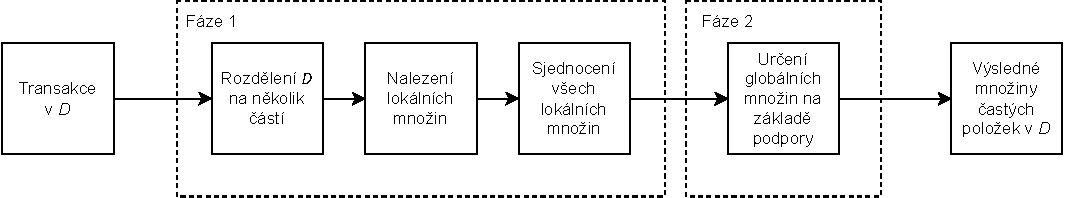
\includegraphics[width=\textwidth]{obrazky-figures/AproiriPart.drawio-crop.pdf}
    \caption{Ilustrace principu techniky rozdělení (partitioning), převzat z~\cite{HanAprioriOpti2012}}
    \label{fig:partitioning_diagram}
\end{figure}


\begin{enumerate}
    \item \textbf{Fáze I:} Databáze je rozdělena do~\( n~\) nepřekrývajících se částí (partitions). Pro~každou z~těchto částí se vypočítá nový lokální práh minimální podpory, definovaný jako \textit{minsup} \(\times\) počet transakcí v~dané části databáze. Dále se pro~každou část nalezne lokální množina častých položek.

    Lokální množina častých položek může, ale nemusí být častá s~ohledem na~celou databázi \( D~\). Nicméně každá množina, která může být potenciálně častá v~celé databázi, se musí vyskytnout jako častá alespoň v~jedné z~částí. Sjednocením častých množin ze všech částí vznikne globální množina kandidátů vůči databázi \( D~\).

    \item \textbf{Fáze II:} Proběhne druhý průchod databází \( D~\), při~kterém je pro~každou kandidátní množinu spočítána její skutečná podpora (\textit{support}) s~cílem určit globálně časté množiny položek. Velikost částí a~jejich počet jsou voleny tak, aby se každá část vešla do~hlavní paměti a~bylo ji možné načíst pouze jednou v~každé fázi.
\end{enumerate}

    \chapter{Návrh a~implementace identifikace s~využitím JA3/JA4 otisků a~frekventovaných vzorů}
\label{chp:design}
Tato kapitola se zaměřuje na~návrh a~implementaci systému pro~identifikaci síťových aplikací s~využitím otisků \textit{JA3} a~\textit{JA4} v~kombinaci s~analýzou frekventovaných vzorů. Nejprve jsou představeny použité datové sady, jejich původ, struktura a~proces předzpracování. Následně je podrobně popsán návrh systému, jeho architektura a~zvolené metody pro~extrakci charakteristických rysů síťové komunikace. Důraz je kladen na~praktickou implementaci řešení, včetně využití algoritmů pro~dolování častých vzorů a~zpracování otisků v~prostředí jazyka \textit{Python}. Cílem této kapitoly je nejen popsat samotný postup realizace systému, ale také zdůvodnit výběr konkrétních technologií a~metod, které byly v~rámci vývoje zvoleny.

\section{Seznámení s~datovými sadami}
\label{sec:dataset}
Pro účely této práce byly poskytnuty tři datové sady: \texttt{mobile\_desktop\_apps\_raw.csv} (autor -- Fakulta informačních technologií, Vysoké učení technické v~Brně ), \texttt{iscx.csv} a~\texttt{iscx-raw.csv} (autor -- Univeristy of New Brunswick, Canadian Institute for Cybersecurity). Tyto soubory obsahují záznamy o~šifrované síťové komunikaci navázané pomocí protokolu \textit{TLS}, konkrétně o~jednotlivých spojeních generovaných různými aplikacemi v~kontrolovaném testovacím prostředí. Každý řádek reprezentuje jedno \textit{TLS} spojení a~popisuje informace získané jak z~klientské zprávy \texttt{Client Hello}, tak ze zprávy \texttt{Server Hello}, které se vyměňují při~navazování šifrovaného spojení.

Datové sady byly využity v~předchozích výzkumech zaměřených na~analýzu šifrovaného provozu a~identifikaci síťových aplikací~\cite{MatousekMobileDevice2020}~\cite{BurgetovaJA42024}. 

Následuje popis jednotlivých souborů:

\begin{itemize}
	\item \textbf{iscx.csv} -- Základní verze datové sady, která obsahuje agregované informace o~spojeních. Klíčové sloupce zahrnují:
	      \begin{itemize}
	      	\item \texttt{SrcIP}, \texttt{DstIP}, \texttt{SrcPort}, \texttt{DstPort} -- informace o~zdrojové a~cílové \textit{IP} adrese a~portech,
	      	\item \texttt{SNI} -- \textit{Server Name Indication}, doménové jméno cílového serveru,
	      	\item \texttt{OrgName}\footnote{OrgName – Organizace odpovídající \textit{IP} adresy serveru, získané z~databáze \textit{WHOIS}.} -- organizace provozující cílový server (např. Google, Skype),
	      	\item \texttt{JA3hash}, \texttt{JA4hash} -- otisky \textit{TLS} klienta dle metod \textit{JA3} a~\textit{JA4},
	      	\item \texttt{JA3Shash}, \texttt{JA4Shash} -- otisky \textit{TLS} serveru dle metod \textit{JA3S} a~\textit{JA4S},
	      	\item \texttt{AppName}\footnote{Nejedná se o~přesné názvy aplikací ale pouze o~jejich zkratky.} -- zkratka názvu aplikace generující provoz (např. Skype, Hangouts),
	      	\item \texttt{Type} -- typ provozu: \texttt{0} (běžná aplikace), \texttt{M} (škodlivý software), \texttt{A} (reklamní či analytický provoz),
	      	\item \texttt{Filename}\footnote{Reprezentuje název souboru, ze kterého byla datová sada poskládána. V~rámci jednoho souboru je zaznamenáno několik spuštění vždy jedné aplikace.} -- název původního souboru, ze kterého byl záznam extrahován,
	      	\item \texttt{Version} -- verze aplikace, (nepoužívaná, vždy \texttt{0}).
	      \end{itemize}
	      	      	      	      	      
	\item \textbf{iscx-raw.csv} -- Rozšířená verze předešlé sady, obsahující detailní \textit{TLS} metadata včetně obsahu jednotlivých \textit{TLS} parametrů:
	      \begin{itemize}
	      	\item \texttt{Proto} -- typ transportního protokolu (např. TCP = \texttt{6}),
	      	\item \texttt{TLSVersion}, \texttt{ClientCipherSuite}, \texttt{ClientExtensions}, \texttt{SignatureAlgorithms}, \texttt{ClientSupportedGroups} -- detailní \textit{TLS} parametry zaslané klientem,
	      	\item \texttt{ServerCipherSuite}, \texttt{ServerExtensions}, \texttt{ServerSupportedVersions} -- odpovídající parametry na~straně serveru,
	      	\item \texttt{JA4\_raw}, \texttt{JA4S\_raw} -- surové podoby otisků.
	      \end{itemize}
	      	      	      	      	      
	\item \textbf{mobile\_desktop\_apps\_raw.csv} -- Podobná struktura jako \texttt{iscx-raw.csv}, avšak data pochází z~oddělené studie zaměřené na~mobilní a~desktopové aplikace~\cite{MatousekMobileDevice2020}. 
	      Přítomny jsou také sloupce jako:
	      \begin{itemize}
	      	\item \texttt{ALPN} -- protokoly vyjednané při~\textit{TLS handshake} (např. \texttt{http/1.1}, \texttt{h2}),
	      	\item \texttt{ClientSupportedVersions} -- seznam verzí \textit{TLS} podporovaných klientem,
	      \end{itemize}
\end{itemize}
Tabulka~\ref{tab:iscx} níže uvádí statistické charakteristiky vybraných atributů obsažených v~datové sadě \texttt{iscx.csv}\footnote{Kromě atributu \texttt{ClientExtensions} jsou všechny uvedené atributy pouze z~datové sady \texttt{iscx.csv}, neboť \texttt{iscx-raw.csv} ji pouze rozšiřuje o~dodatečná metadata.}. Pro~každý atribut je uveden počet unikátních hodnot, podíl unikátních hodnot vůči celkovému počtu záznamů (v\,\%), celkový počet výskytů atributu, podíl výskytů vzhledem k~celkovému počtu řádků v~datové sadě (v\,\%). Tato statistika slouží k~posouzení informační hodnoty jednotlivých atributů pro~účely identifikace.
\begin{table}[H]
	\centering
	\begin{tabular}{lrlrl}
		\toprule
		\textbf{Položky} & \textbf{Počet unikátních hodnot} & \textbf{( v\,\%)} & \textbf{Celkový počet} & \textbf{( v\,\%)} \\
		\midrule
		SNI               & 207                                 & 8{,}50            & 2092                     & 85{,}88           \\
		OrgName           & 72                                  & 2{,}96            & 2300                     & 94{,}42           \\
		ClientExtensions  & 32                                  & 1.31              & 2436                     & 100.00            \\
		JA3hash           & 46                                  & 1{,}89            & 2436                     & 100{,}00          \\
		JA4hash           & 42                                  & 1{,}72            & 2436                     & 100{,}00          \\
		AppName           & 16                                  & 0{,}66            & 2436                     & 100{,}00          \\
		JA3Shash          & 117                                 & 4{,}80            & 2399                     & 98{,}48           \\
		JA4Shash          & 127                                 & 5{,}21            & 2399                     & 98{,}48           \\
		Filename          & 109                                 & 4{,}47            & 2399                     & 98{,}48           \\
		Type              & 2                                   & 0.08              & 2436                     & 100.00            \\
		\bottomrule
	\end{tabular}
	\caption{Přehled položek v~datové sadě \texttt{iscx.csv}}
	\label{tab:iscx}
\end{table}

Tabulka~\ref{tab:mobile} rozšiřuje statistickou analýzu na~datovou sadu \texttt{mobile\_desktop\_apps\_raw}. Opět jsou uvedeny klíčové atributy relevantní pro~identifikaci aplikací.

\begin{table}[H]
	\centering
	\begin{tabular}{lrlrl}
		\toprule
		\textbf{Položky} & \textbf{Počet unikátních hodnot} & \textbf{( v\,\%)} & \textbf{Celkový počet} & ( \textbf{v\,\%)} \\
		\midrule
		SNI               & 929                                 & 4.36              & 21259                    & 99.80             \\
		OrgName           & 197                                 & 0.92              & 21273                    & 99.87             \\
		ClientExtensions  & 10462                               & 49.12             & 21301                    & 100.00            \\
		ALPN              & 9                                   & 0.04              & 19505                    & 91.57             \\
		JA3hash           & 10495                               & 49.27             & 21301                    & 100.00            \\
		JA4hash           & 123                                 & 0.58              & 21301                    & 100.00            \\
		AppName           & 78                                  & 0.37              & 21301                    & 100.00            \\
		JA3Shash          & 83                                  & 0.39              & 21180                    & 99.43             \\
		JA4Shash          & 103                                 & 0.48              & 21180                    & 99.43             \\
		Filename          & 1746                                & 8.20              & 21180                    & 99.43             \\
		Version           & 1                                   & 0.00              & 21180                    & 99.43             \\
		\bottomrule
	\end{tabular}
	\caption{Přehled položek v~datové sadě \texttt{mobile\_desktop\_apps\_raw.csv}}
	\label{tab:mobile}
\end{table}

V prvních dvou datových sadách, \texttt{iscx.csv} a~\texttt{iscx-raw.csv}, se nachází \textbf{celkem 2436 záznamů}, které byly vygenerovány \textbf{16 různými aplikacemi}. Tyto záznamy pocházejí ze \textbf{109 různých spuštění} (atribut \textit{Filename}). Otisky \textit{JA3} a~\textit{JA4} jsou dostupné pro~každý záznam, zatímco otisky \textit{JA3S} a~\textit{JA4S} chybí přibližně u~1,52\,\% záznamů.

Lze si rovněž povšimnout, že atribut \textit{SNI}, ačkoliv chybí u~14,12\,\% záznamů, obsahuje \textbf{největší počet unikátních hodnot}. Díky tomu se jeví jako ideální kandidát pro~přesnější identifikaci aplikací -- zejména v~případech, kdy dochází ke~zlepšení identifikace kombinací více atributů.

Datová sada \texttt{mobile\_desktop\_apps\_raw.csv} obsahuje \textbf{celkem 21301 záznamů}, které byly vygenerovány \textbf{78 různými aplikacemi}. Dále zahrnuje \textbf{1746 odlišných spuštění} (atribut \texttt{Filename}). Stejně jako u~předchozích datových sad nechybí žádný z~otisků \textit{JA3} ani \textit{JA4}. Naopak otisky \textit{JA3S} a~\textit{JA4S} chybí ve~0,57\,\% případů.

Zajímavý je poměr počtu otisků \textit{JA3} ku~\textit{JA4}, který činí přibližně \textbf{85:1} (10495 ku~123). Tento výrazný nepoměr naznačuje, že informační hodnota otisků \textit{JA3} může být silně ovlivněna přímo použitými rozšířeními (např. \texttt{ClientExtensions}), kterých je v~datasetu evidováno 10462, viz~\ref{sec:JA3}. Na~rozdíl od~\textit{JA4}, jehož konstrukce počítá s~filtrováním redundancí pomoci seřazení a~výpočtu zkráceného hashe, se \textit{JA3} otisk generuje ze všech rozšíření bez~jakýchkoli úprav, což může vést ke~snížení jeho spolehlivosti pro~účely identifikace.

Opět i~v~tomto případě se položka \textit{SNI} jeví jako \textbf{vhodný kandidát pro~přesnější identifikaci}, neboť vykazuje vysoký počet unikátních hodnot a~chybí pouze ve~0,2\,\% záznamů, což svědčí o~její vysoké informační hodnotě.

Tabulky~\ref{tab:apps-iscx} a~\ref{tab:apps-mobile} poskytují přehled o~rozložení aplikací v~jednotlivých použitých datových sadách. Každá tabulka uvádí název aplikace, počet zaznamenaných spojení a~relativní podíl na~celkovém počtu spojení v~dané datové sadě.
Tabulka~\ref{tab:apps-iscx} shrnuje statistiky z~datové sady \texttt{iscx.csv}, kde dominují zejména aplikace jako \textit{Hangouts} a~\textit{Skype}.
Taktéž tabulka~\ref{tab:apps-mobile} zachycuje rozložení aplikací v~rozsáhlejší datové sadě \texttt{mobile\_desktop\_apps\_raw.csv}, která obsahuje širší spektrum moderních mobilních i~desktopových aplikací.

Pro přehlednost jsou v~obou tabulkách uvedeny pouze vybrané položky -- prostřední části byly nahrazeny výpustkami.

\begin{table}[H]
	\centering
	\begin{minipage}{0.49\textwidth}
		\centering
		\begin{tabular}{lll}
			\toprule
			\multicolumn{3}{c}{\texttt{iscx.csv}} \\
			\midrule
			\textbf{Aplikace} & \textbf{Počet} & \textbf{Podíl (\%)} \\
			\midrule
			Hangouts          & 553             & 22.70                \\
			Skype             & 436             & 17.90                \\
			Email             & 315             & 12.93                \\
			\vdots            & \vdots          & \vdots               \\
			SCP               & 9               & 0.37                 \\
			BitTorrent        & 8               & 0.33                 \\
			ICQ               & 7               & 0.29                 \\
			\bottomrule
		\end{tabular}
		\caption{Přehled aplikací v~\texttt{iscx.csv}}
		\label{tab:apps-iscx}
	\end{minipage}
	\hfill
	\begin{minipage}{0.49\textwidth}
		\centering
		\begin{tabular}{lll}
			\toprule
			\multicolumn{3}{c}{\texttt{mobile\_desktop\_apps\_raw.csv}} \\
			\midrule
			\textbf{Aplikace} & \textbf{Počet} & \textbf{Podíl (\%)} \\
			\midrule
			AirDroid          & 1774            & 8.33                 \\
			Oer               & 1441            & 6.76                 \\
			BiduTerBox        & 1252            & 5.88                 \\
			\vdots            & \vdots          & \vdots               \\
			Milbird           & 15              & 0.07                 \\
			Telegram          & 12              & 0.06                 \\
			TelegramDesktop   & 1               & 0.01                 \\
			\bottomrule
		\end{tabular}
		\caption{Přehled aplikací v~3. sadě}
		\label{tab:apps-mobile}
	\end{minipage}
\end{table}


Všechny tři datové sady se všemi atributy, včetně kompletního seznamu aplikací použitých v~těchto sadách, jsou uvedeny v~příloze~\ref{chp:appendix-ds}.


\section{Motivace a~obecný popis}
Tato sekce poskytuje obecný přehled o~navrženém řešení, jeho struktuře a~zvoleném přístupu. Hlavním cílem této práce je zlepšit identifikaci aplikací prostřednictvím kontextového přístupu. Při~aplikaci otisku na~identifikované spojení je vygenerována kandidátní množina aplikací, tedy množina všech aplikací, ke~kterým je daný otisk přiřazen v~trénovací fázi. Tato kandidátní množina je tedy výsledkem metod, jako jsou \textit{JA3} nebo \textit{JA4}, pokud jsou použity k~identifikaci \textit{TLS} spojení. Identifikace založená výhradně na~otiscích, přestože může na~první pohled působit poměrně přesně, není ideální – průměrná velikost kandidátní množiny bývá často příliš rozsáhlá, což snižuje její informační hodnotu.

Například v~situaci, kdy 16 odlišných aplikací generuje síťovou komunikaci, může klasifikace založená na~otiscích vrátit kandidátní množinu o~velikosti 14. Takový výsledek je z~hlediska jednoznačné identifikace aplikace prakticky bezcenný, protože neposkytuje dostatečně úzký výběr možných odpovědí. 

Cílem této práce je pokusit se zúžit kandidátní množinu tak, aby bylo možné dosáhnout přesnější identifikace aplikace, a~to na~základě kontextu dalších \textit{TLS} spojení, která se vyskytují paralelně s~daným spojením. Využití kontextu dalších \textit{TLS} spojení je možné díky tomu, že většina aplikací při~spuštění generuje více souběžných spojení~\cite{tls-mulitple-conns}. V~rámci těchto okolních \textit{TLS} spojení se hledají frekventované vzory, založené na~otiscích a~případně i~dalších atributech komunikace. Na~základě shody mezi~aktuálním okolím spojení a~předem známými frekventovanými vzory je následně možné určit nejpravděpodobnější kandidáty pro~identifikaci aplikace. 

\section{Návrh řešení}
Tato kapitola se věnuje detailnímu návrhu systému. Na~základě analýzy současných metod a~problémů spojených s~identifikací na~základě otisků je zde představen nový přístup, který využívá informace o~souběžně navázaných \textit{TLS} spojeních.

Cílem návrhu je vytvořit systém, který dokáže efektivně využít kontextové informace k~zúžení kandidátní množiny aplikací, a~tím zlepšit přesnost výsledné identifikace. Sekce popisuje požadavky na~systém, jeho architekturu, zvolené algoritmy a~metodiky, předpoklady pro~jeho fungování i~jednotlivé klíčové části řešení.


\subsection{Požadavky a~cíle}

Jak již bylo zmíněno, hlavním cílem této práce je především zúžení kandidátní množiny pomocí kontextového přístupu. Zároveň je žádoucí, aby byla zachována co nejvyšší přesnost identifikace a~aby zpracování spojení nebylo časově náročné. Je proto nutné nalézt ideální kompromis mezi~přesností a~časovou náročností, což samo o~sobě může být náročné.

\subsection{Architektura systému}
\label{sub:architecture}
Z~důvodu rozšiřitelnosti a~snadnější manipulace byl zvolen přístup objektově orientovaného programování. Systém je rozdělen do~několika vzájemně spolupracujících tříd, které odpovídají jednotlivým částem řešení – načítání a~uchovávání dat, identifikace založená čistě na~otiscích, učení frekventovaných vzorů a~kombinace identifikace otisků s~kontextovým přístupem. Součástí systému jsou i~třídy pro~logování, správu nastavení a~parsování parametrů z~příkazové řádky. Tento přístup zajišťuje lepší modularitu, snadnější rozšiřování funkcionality a~přehlednou správu celkového kódu. Diagram tříd~\ref{fig:class-dia} poskytuje podrobný přehled jednotlivých tříd a~jejich metod.

\begin{figure}[H]
	\centering
	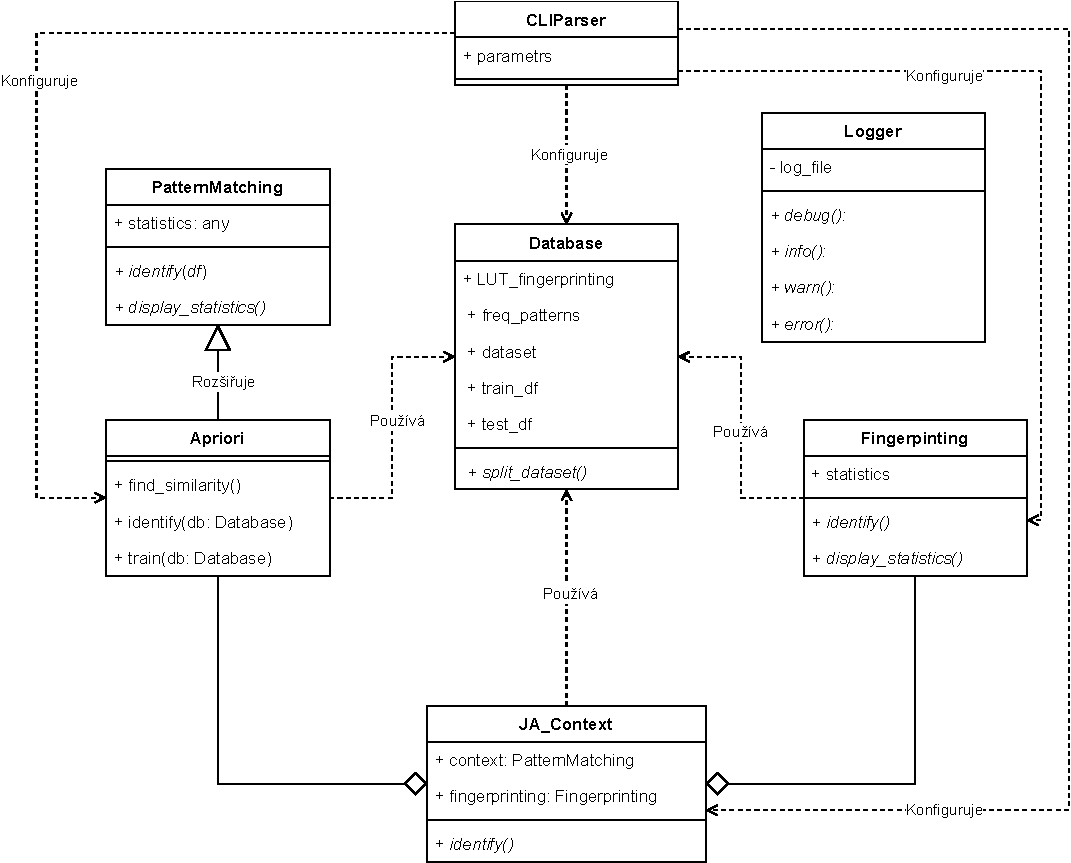
\includegraphics[width=\textwidth]{obrazky-figures/class-dia.drawio.pdf}
	\caption{Diagram tříd}
	\label{fig:class-dia}
\end{figure}


V příloze~\ref{chp:appendix-class-diagram} je uvedena rozšířená verze diagramu tříd, která obsahuje všechny atributy a~metody.

Navržené řešení se bude skládat ze sedmi tříd, přičemž každá z~nich pokryje jasně vymezenou část systému. Ovládání systému bude zajištěno prostřednictvím příkazové řádky, což vyžaduje existenci třídy \texttt{CLIParser}, která zpracuje parametry programu a~předá je příslušným instancím ostatních tříd, jak je znázorněno v~diagramu~\ref{fig:class-dia}.

Pro účely snadného ladění a~lepšího porozumění běhu programu se každý významný krok bude zaznamenávat prostřednictvím instance třídy \texttt{Logger}.

Třída \texttt{Database} bude sloužit jako hlavní zdroj dat a~poskytne přístup k~vyhledávací tabulce otisků, datové struktuře frekventovaných vzorů a~dalším potřebným údajům z~trénovací i~testovací části datové sady. Přístup k~těmto datům bude mít každá komponenta, která je bude vyžadovat.

Třída \texttt{Fingerprinting} nabídne metody pro~identifikaci \textit{TLS} spojení pomocí otisků \textit{JA3}, \textit{JA4} či jejich kombinací (\textit{JA} + \textit{JAS} + \textit{SNI}), přičemž bude využívat vyhledávací tabulku uloženou v~databázi. Zároveň bude zajišťovat generování statistik, které zaznamenají například přesnost identifikace nebo velikost kandidátní množiny.

Třída \texttt{PatternMatching} vytvoří základní rozhraní pro~implementaci algoritmů určených k~dolování informací z~dat. Její návrh umožní snadné rozšíření systému o~další metody data miningu a~zajistí tak jeho flexibilitu a~rozšiřitelnost.

Třída \texttt{Apriori} rozšíří třídu \texttt{PatternMatching} o~konkrétní implementaci algoritmu \textit{Apriori}. Tento algoritmus umožní vyhledávání frekventovaných vzorců v~trénovacích datech a~bude spolupracovat s~databází pro~jejich ukládání a~vyhledávání. Porovnávat nalezené vzory se zkoumaným \textit{TLS} spojením a~vracet N\footnote{Kde N~reprezentuje předem určený maximální počet kandidátů.} nejpravděpodobnějších kandidátů na~základě podobnosti, vypočítané například porovnáním otisků nebo frekvence vzorců, bude metoda \texttt{find\_similarity()}.

Třída \texttt{JA\_Context} bude koordinovat využití tříd \texttt{Apriori} a~\texttt{Fingerprinting} s~cílem zúžit kandidátní množinu pro~identifikaci aplikace. Nejprve provede iteraci přes testovací data v~rámci předem definovaného okna a~tím specifikuje okolí analyzovaného spojení. Pomocí otisků vytvoří počáteční kandidátní množinu aplikací, které budou relevantní pro~dané spojení. Následně předá odpovídající frekventované vzory těchto kandidátů instanci třídy \texttt{Apriori}, která se pokusí nalézt vzory charakteristické pro~aplikace v~dané oblasti. Výsledkem tohoto procesu bude dále zúžená kandidátní množina obsahující aplikace nejlépe odpovídající analyzovanému spojení.

\subsection{Předpoklady a~omezení}
Pro správné spuštění a~fungování systému je nutné splnit několik základních předpokladů:
\begin{itemize}
	\item \textbf{Dostupnost datové sady}: Program vyžaduje existenci pojmenované datové sady obsahující alespoň čtyři TLS spojení, přičemž každé musí obsahovat otisky \textit{JA3} a~\textit{JA3S} (případně \textit{JA4} a~\textit{JA4S}) a~atribut \textit{SNI}. Bez~datové sady nebude možné program spustit.
	\item \textbf{Kvalita a~rozsah dat}: Platí, že čím více unikátních spuštění aplikací je v~datové sadě zaznamenáno, tím rozsáhlejší a~přesnější frekventované vzory je možné extrahovat. Malé množství dat povede ke~snížení přesnosti identifikace. Ovšem také velmi rozsáhlé datové sady mohou zvýšit nároky na~paměť a~výpočetní výkon. Návrh systému je optimalizován pro~běžné datové sady (například \texttt{mobile\_desktop\_apps\_raw.csv}, která obsahuje 21,301 řádků, je v~tomto případě považována za~běžnou datovou sadu).
\end{itemize}

\section{Implementace}
Tato sekce popisuje implementační detaily, použité technologie a~poskytuje podrobný popis klíčových částí systému.

\subsection{Použité technologie a~nástroje}
Pro implementaci byl zvolen programovací jazyk \textit{Python} verze 3.13 kvůli vysoké flexibilitě a~dostupnosti knihoven jak pro~práci s~daty, tak pro~matematické výpočty a~další účely. \textit{Python} také usnadňuje implementaci objektově orientovaného návrhu.

Za účelem efektivní práce s~datovou sadou byla zvolena knihovna \textit{Pandas} verze 2.2.3. Algoritmus \textit{Apriori} byl importován z~knihovny \textit{mlxtend} verze 0.23.4, stejně jako \textit{TransactionEncoder}, který je potřebný pro~předzpracování dat. Knihovna \textit{scikit\_learn} verze 1.6.1 poskytla metodu \texttt{train\_test\_split} pro~rozdělení datové sady na~testovací a~trénovací část, a~také metodu \texttt{cosine\_similarity} pro~výpočet kosinové podobnosti. Knihovna \textit{numpy} verze 2.2.5 byla také využita pro~různé matematické operace. Při tvorbě této technické zprávy byla využita umělá inteligence, konkrétně \textit{ChatGPT}, pro úpravu stylistiky a opravu gramatiky.


\subsection{Použití programu a~konfigurace}
K zajištění správného běhu programu a~korektního zpracování dat byl vytvořen konfigurační soubor \texttt{config.py}, ve~kterém lze upravovat jednotlivé názvy sloupců v~případě použití jiných datových sad. V~tomto souboru lze také povolit ladicí výpisy, které budou propsány do~logů. Byl umístěn na~stejné úrovni zanoření jako \texttt{main.py}, pomocí kterého se celý program spouští. Všechny navrhované třídy jsou implementovány v~jednotlivých souborech ve~složce \texttt{identify}, s~výjimkou tříd \texttt{PatternMatching} a~\texttt{Apriori}, které jsou implementovány v~jednom společném souboru. Struktura celého projektu je uvedena v~příloze~\ref{chap:appendix-structure}.
Program lze spustit následujícím příkazem:

\begin{lstlisting}[language=bash]
python3 main.py -d <ds> -f <3|4> -w <win> -m <min_sup> -c <num_can>
\end{lstlisting}

Kde:
\begin{itemize}
	\item \texttt{-d <ds>}: Reprezentuje cestu k~datové sadě (např. \texttt{data/iscx.csv}),
	\item \texttt{-f <3|4>}: Volí verzi otisků (\texttt{3} pro~\textit{JA3}, \texttt{4} pro~\textit{JA4}),
	\item \texttt{-w <win>}: Určuje šířku posuvného okna (celé číslo),
	\item \texttt{-m <min\_sup>}: Specifikuje minimální podporu pro~\textit{Apriori} (desetinné číslo v~rozsahu 0{,}0–1{,}0),
	\item \texttt{-c <num\_can>}: Nastavuje počet kandidátů ve~množině (celé číslo), 
	\item a~\texttt{-h}, \texttt{--help}: Zobrazí nápovědu.
\end{itemize}

\subsection{Popis klíčových částí}
\label{subsec:klicove}
Tato podsekce popisuje klíčové a~zajímavé části programu, které se objevily v~průběhu implementace. 

\subsubsection{Rozdělení a~čištění datové sady}
Nejprve dochází k~čištění datové sady, během něhož jsou odstraněny všechny záznamy typu \texttt{A} a~\texttt{M} reprezentující reklamní provoz či malware. Tímto krokem se zachovají pouze záznamy odpovídající běžnému provozu. Následně je datová sada rozdělena v~poměru 75:25 na~trénovací a~testovací část.

Rozdělení probíhá na~základě hodnoty atributu \texttt{Filename}, který reprezentuje jednotlivá spuštění aplikací. V~rámci každého spuštění je 75\% záznamů zařazeno do~trénovací množiny a~zbývajících 25\% do~množiny testovací. Tím je zajištěno, že každé spuštění je zastoupeno v~obou částech sad.

Pokud dané spuštění obsahuje pouze jeden záznam (tj. daná aplikace vygenerovala pouze jedno \textit{TLS} spojení), je tento záznam přiřazen automaticky do~trénovací části, aby bylo možné z~něj vytěžit potřebné vzory.

\subsubsection{Těžba frekventovaných vzorů}

Spojení v~tomto kroku jsou reprezentována jako kombinace několika diskrétních hodnot, zejména otisků \textit{JA3}, \textit{JA3S}, \textit{JA4}, \textit{JA4S}, a~dále atributů jako \textit{SNI} nebo \textit{OrgName}. Tyto prvky slouží jako základní položky pro~tvorbu transakcí, nad~nimiž je následně aplikován algoritmus \textit{Apriori} k~identifikaci často se vyskytujících vzorů charakteristických pro~jednotlivé aplikace.

Před samotnou aplikací algoritmu jsou data převedena do~binární reprezentace pomocí objektu \texttt{TransactionEncoder} z~knihovny \texttt{mlxtend}, který transformuje kategorická data do~formátu, se kterým algoritmus \textit{Apriori} pracuje. Následně je volána funkce \texttt{apriori()}, která na~základě zadané minimální podpory (\texttt{min\_support}) vyhledá všechny časté vzory, jež se vyskytují ve~spojeních dané aplikace.

Algoritmus \textit{Apriori} se aplikuje na~trénovací část datové sady, konkrétně na~seskupená data podle jednotlivých aplikací, pro~které se frekventované vzory vyhledávají. Následně jsou všechny nalezené vzory očištěny na~základě parametrů, které budou popsány v~následující kapitole~\ref{chp:exps} v~rámci experimentů.

Výsledkem tohoto kroku je pro~každou aplikaci množina častých vzorů, které jsou dále použity v~kontextové fázi identifikace, kde slouží k~porovnání s~okolními spojeními.

\subsubsection{Volba kontextu identifikovaného spojení}

Identifikace probíhá nad~testovacími daty, která jsou seskupena za~sebou podle jednotlivých spuštění aplikací. Tyto skupiny jsou následně deterministicky promíchány v~takovém pořadí, aby žádné dvě po~sobě jdoucí skupiny nepocházely od~stejné aplikace. Toto opatření má za~cíl předejít příliš výraznému kontextu, který by mohl zkreslit výsledky. Cílem je simulovat realistický scénář běžného provozu, kdy je pravděpodobnost opakovaného spuštění stejné aplikace bezprostředně po~sobě relativně nízká.

Kontext, neboli okolí zkoumaného spojení, se určuje pomocí posuvného okna (angl. sliding window) s~předem definovanou šířkou, které iteruje přes celou testovací část dat. Velikost okna by ideálně měla být lichá, aby bylo možné udržet zkoumané spojení uprostřed a~zároveň zajistit symetrický počet sousedních spojení na~obou stranách. V~případech, kdy se zkoumané spojení nachází příliš blízko začátku nebo konce testovací sady a~běžné centrování by vedlo k~neúplnému oknu, je pozice spojení v~rámci okna upravena tak, aby bylo možné zachovat úplný a~vyvážený kontext. V~takových situacích zůstává pozice okna v~datech pevná a~posouvá se pouze relativní umístění zkoumaného spojení uvnitř tohoto okna.

Velikost posuvného okna má zásadní vliv na~kvalitu identifikace. Příliš malé okno nemusí zachytit dostatečný kontext pro~spolehlivé porovnání s~frekventovanými vzory, což vede ke~ztrátě informační hodnoty. Naopak příliš široké okno může zahrnout irelevantní nebo rušivé spojení od~jiných aplikací, čímž dochází ke~zhoršení přesnosti. Z~tohoto důvodu je volba optimální velikosti okna předmětem experimentálního vyhodnocení, které je popsáno v~sekci~\ref{sec:ex-window}.

\subsubsection{Výpočet podobnosti}
Při identifikaci se ve~zkoumaném kontextu vyhledávají frekventované vzory jednotlivých aplikací. Pouhé přesné porovnání těchto vzorů však není efektivní, protože často dochází k~částečnému překryvu mezi~kontextem a~naučenými vzory. Vhodnějším přístupem je proto výpočet míry podobnosti mezi~množinami prvků -- tedy mezi~frekventovanými vzory dané aplikace a~aktuálním obsahem kontextového okna.

Tato podobnost byla zprvu kvantifikována pomocí metriky kosinové podobnosti, která umožňuje zohlednit nejen přesné shody, ale i~dílčí překryvy. Později se však ukázalo, že při~rozsáhlé databázi vzorů a~velkém počtu spojení není její časová náročnost ideální. Mnohem příznivější výsledky z~hlediska výpočetní efektivity přinesly množinové operace, jako například \textit{Jaccardova} či \textit{Diceho} podobnost. Výsledkem je \uv{skóre} podobnosti pro~každou aplikaci, na~jehož základě je následně sestavena kandidátní množina nejpravděpodobnějších aplikací.

Samotný výpočet skóre probíhá následovně: pro~každou aplikaci se prochází seznam jejích frekventovaných vzorů. Každý vzor je reprezentován jako množina položek (např. kombinace \textit{JA3}, \textit{SNI} a~\textit{JA4S}), a~jeho výskyt je zaznamenán napříč celou trénovací množinou. Následně je vypočteno skóre relevance vůči aktuálnímu \textit{TLS} spojení na~základě \textit{Jaccardovy} podobnosti mezi~vzorem a~zkoumanou množinou obsahující atributy spojení. \textit{Jaccardova} podobnost je vyobrazena v~rovnici~\ref{eq:jacc}.
\begin{equation}
	J(A, B) = \frac{|A \cap B|}{|A \cup B|}
    \label{eq:jacc}
\end{equation}
Tento dílčí výsledek je dále upraven pomocí \textit{IDF} faktoru, který zvýhodňuje méně časté vzory podle vztahu~\ref{eq:idf}:
\begin{equation}
	\text{idf}(p) = \log\left(1 + \frac{N}{\text{df}(p)}\right)
    \label{eq:idf}
\end{equation}
kde \( N~\) je celkový počet aplikací a~\( \text{df}(p) \) je počet aplikací obsahujících daný vzor \( p~\), jak je zapsáno rovnicí~\ref{eq:s1}.

Pokud je vzor podmnožinou atributů spojení, skóre se ještě násobí podporou vzoru a~jeho délkou, viz~\ref{eq:s2}, což zvýhodňuje přesné a~zároveň delší shody. Výsledná skóre všech aplikací jsou nejprve normalizována pomocí \textit{min-max} normalizace, aby bylo možné jednotlivé hodnoty porovnávat na~stejné škále. Následně jsou nejpravděpodobnější kandidáti určeni na~základě nejvyšších skóre -- k~jejich efektivnímu výběru se využívá funkce \texttt{heapq.nlargest}, která díky použití haldy umožňuje rychlý výběr \texttt{N} nejlépe hodnocených položek bez~nutnosti seřadit celý seznam. 


\paragraph{Výpočet skóre podobnosti}

Skóre aplikace \( a~\) je počítáno jako vážený součet příspěvků jednotlivých vzorů \( p~\in P_a \), viz~\ref{eq:score}:

\begin{enumerate}
	\item \textbf{Základní skóre pomocí \textit{Jaccardovy} podobnosti:}
	      \begin{equation}
	      	s_1(p, C) = \left( J(p, C) + 1 \right) \cdot \mathrm{idf}(p)
	      	\label{eq:s1}
	      \end{equation}
	\item \textbf{Doplňkové skóre při~úplné shodě (podmnožině):}
	      \begin{equation}
	      	s_2(p, C) = 
	      	\begin{cases}
	      		|p| \cdot 10 \cdot \mathrm{idf}(p) \cdot (\mathrm{sup}_\mathrm{norm}(p) + 1), & \text{pokud } p~\subseteq C~\\
	      		0,                                                                            & \text{jinak}                
	      	\end{cases}
	      	\label{eq:s2}
	      \end{equation}
	\item \textbf{Celkové skóre aplikace \( a~\):}
	      \begin{equation}
	      	\mathrm{score}(a) = \sum_{p \in P_a} \left[ s_1(p, C) + s_2(p, C) \right]
	      	\label{eq:score}
	      \end{equation}
\end{enumerate}

\noindent
kde:
\begin{itemize}
	\item \( P_a \) je množina frekventovaných vzorů pro~aplikaci \( a~\),
	\item \( C~\) je množina atributů kontextu,
	\item \( J(p, C) \) je \textit{Jaccardova} podobnost mezi~vzorem \( p~\) a~kontextem \( C~\),
\end{itemize}

V případě, že první fáze identifikace (využití samotných otisků bez~kontextu) vrátí kandidátní množinu požadované délky, je i~přesto proveden výpočet podobnosti. Pokud již nedojde ke~zkrácení množiny, slouží tento výpočet alespoň k~jejímu seřazení podle nejpravděpodobnější aplikace.

Je také možné, že první fáze identifikace neposkytne žádné kandidátní aplikace, použije se pro~vyhledávání v~kontextu celá databáze frekventovaných vzorů. Pokud ani v~okolí daného spojení (v rámci daného kontextu) nebude nalezen žádný frekventovaný vzor odpovídající zúžené databázi, provede se rozšíření vyhledávání i~na~vzory aplikací, které tvoří komplement původní množiny. Tento postup zajišťuje, že bude vždy existovat alespoň pokus o~identifikaci, i~v~případech, kdy selže primární výběr podle otisků.

\subsubsection{Vyhodnocení úspěšnosti}

Identifikace je vyhodnocována na~základě pevně zvoleného počtu kandidátů \( N~\). Pro~každou pozici \( x~\), kde \( x~\leq N\), je zaznamenána úspěšnost -- tedy podíl případů, kdy se skutečná aplikace nachází na~dané pozici v~kandidátní množině. Jinými slovy, pokud je hodnota \( N~\) nastavena na~3, jsou vyhodnoceny statistiky přesnosti pro~1., 2. a~3. pozici výsledné kandidátní množiny. Celková úspěšnost je počítána jako součet dílčích úspěšností pro~jednotlivé pozice v~kandidátní množině. Chybovost je následně vyjádřena jako doplněk celkové úspěšnosti do~jedné. Kromě toho jsou vypočítávány i~charakteristiky velikosti kandidátních množin, jako je průměr, medián a~modus. Tyto metriky umožňují posoudit nejen přesnost identifikace, ale i~kompaktnost výsledných množin, což je zásadní pro~praktickou použitelnost a~analýzu navrženého systému.

\section{Zhodnocení návrhu a~rozdíly v~implementaci}


Navržená architektura systému byla převážně dodržena, včetně rozdělení systému do~samostatných tříd. Objektový návrh se osvědčil zejména při~udržování přehlednosti a~při~výraznějších změnách v~kódu. Některé třídy však byly oproti původnímu návrhu mírně rozšířeny – například třída \texttt{Fingerprinting} byla doplněna o~dodatečné statistiky. Naopak některé pomocné funkce byly z~důvodu přehlednosti nebo znovupoužitelnosti přesunuty mimo své původní třídy.

Při implementaci bylo nutné učinit několik kompromisů. Nejvýraznějším z~nich byla nutnost nahradit původně zamýšlené výpočetně náročnější metriky pro~výpočet podobnosti jednoduššími množinovými operacemi. Konkrétně došlo k~nahrazení kosinové podobnosti \textit{Jaccardovou} podobností, což přineslo výrazné zrychlení a~umožnilo splnit nefunkční požadavek na~časovou náročnost, a~to i~přes zanedbatelné zhoršení přesnosti identifikace.

Mezi hlavní výzvy patřila práce s~rozsáhlými datovými sadami, zejména při~opakovaném trénování algoritmu \textit{Apriori} pro~desítky různých aplikací. Bylo nutné optimalizovat datové struktury a~přistupovat k~datům selektivně. Dále bylo důležité nalézt vhodný kompromis mezi~přesností identifikace a~rychlostí zpracování. Počet vytěžených častých vzorů na~aplikaci se oproti navrhovanému řešení snížil na~pouhé desítky.

Možnosti budoucího rozšíření zahrnují paralelizaci dat, což by umožnilo rychlejší trénování a~hodnocení na~více-jádrových systémech. Dalším krokem by mohlo být přidání algoritmu \textit{FP-Growth} nebo úplné nahrazení algoritmu \textit{Apriori}. Také by bylo možné zkoumat alternativní metriky podobnosti nebo zavést váhování jednotlivých atributů podle jejich informační hodnoty. V~neposlední řadě lze systém doplnit o~heuristiky pro~automatickou kalibraci parametrů nebo o~adaptivní učení na~nových datech.

    \chapter{Experimenty za~účelem zlepšení identifikace}
\label{chp:exps}

Tato kapitola představuje soubor experimentů zaměřených na~zefektivnění procesu identifikace aplikací. Hlavním cílem je minimalizace mohutnosti kandidátní množiny aplikací při~současném zachování co nejvyšší přesnosti. Zároveň jsou respektovány všechny relevantní nefunkční požadavky, zejména s~ohledem na~časovou náročnost.

Identifikace a~použití otisků probíhá ve dvou fázích, jak bylo popsáno v~sekci~\ref{sub:architecture}. Nejprve je aplikována metoda fingerprintingu \textit{JA3}, \textit{JA4} či jejich kombinace, na~jejímž základě je získána kandidátní množina (proběhne jednoduché vyhledání aplikací, které odpovídají danému otisku). Tato množina kandidátů je dále v~textu označována jako \textbf{počáteční kandidátní množina}.

Počáteční kandidátní množina přímo určuje, které získané vzory (tj. vzory získané z~trénovací množiny) se budou používat pro~výpočet podobnosti. V~modelové situaci je pro~dané spojení vygenerována počáteční kandidátní množina obsahující \texttt{App1}, \texttt{App2} a~\texttt{App3}. Výpočet podobnosti mezi~kontextem daného spojení a~frekventovanými vzory tedy probíhá pouze pro~vzory aplikací \texttt{App1}, \texttt{App2} a~\texttt{App3}.

Tímto způsobem se zefektivní identifikace aplikací, jelikož není potřeba iterovat přes časté vzory, které nejsou v~počáteční kandidátní množině. Použití kontextu zde slouží pouze ke~zúžení kandidátní množiny. Tato množina bude dále v~textu označována jako \textbf{finální kandidátní množina}.

\section{Volby položek pro~získání vzorů}
\label{sec:ex1}
Cílem tohoto experimentu je vyhodnotit, které otisky a~případně další atributy spojení, například \textit{SNI} či \textit{ORG}, přinášejí nejvyšší přesnost identifikace, a~to jak při~tvorbě počáteční kandidátní množiny, tak i~jako vstupní data pro~algoritmus \textit{Apriori}. Ideální kombinace by zároveň měla generovat co nejkratší finální kandidátní množinu aplikací a~udržet výpočetní náročnost v~přijatelných mezích.

Pro tyto experimenty byly ostatní parametry zvoleny následovně: \textbf{minimální podpora} algoritmu \textit{Apriori} byla nastavena \textbf{na 0{,}25}, \textbf{počet finálních kandidátů na~3}, \textbf{šířka okna na~15} spojení u~sady \texttt{iscx.csv} a~\textbf{25} u~sady \texttt{mobile-desktop-apps-raw.csv}. Metody generující počáteční kandidátní množinu byly: \textit{JA3}, \textit{JA3+JA3S+SNI}, \textit{JA4} a~\textit{JA4+JA4S+SNI}.

Tabulka \ref{tab:fingerprints-accuracy} shrnuje přesnost a~průměrnou délku počáteční kandidátní množiny po~aplikaci metod \textit{JA3}, \textit{JA4} a~jejich kombinací. Výsledky odpovídají čistému fingerprintingu daných spojení, tedy bez~využití kontextu a~frekventovaných vzorů. Tabulka slouží jako výchozí přehled přesnosti základního fingerprintingu na~jednotlivých datových sadách a~jako referenční bod pro~následné porovnání s~výsledky identifikace využívající kontext. 

\begin{table}[H]
	\centering
	\begin{tabular}{lrrrr}
		\toprule
		\multirow{2}*{\textbf{Otisky}}&\multicolumn{2}{c}{\texttt{iscx.csv}} & \multicolumn{2}{c}{\texttt{mobile\_desktop\_apps\_raw.csv}} \\
		             & \textbf{Přesnost} & \textbf{Délka} & \textbf{Přesnost} & \textbf{Délka} \\
		\midrule
		JA3          & 0.975              & 3.146           & 0.495              & 4.325           \\
		JA3+JA3S+SNI & 0.924              & 2.099           & 0.855              & 5.953           \\
		JA4          & 0.975              & 3.146           & 0.966              & 14.298          \\
		JA4+JA4S+SNI & 0.924              & 2.094           & 0.854              & 3.382           \\
		\bottomrule
	\end{tabular}
	\caption{Přesnost otisků a~jejich kombinací}
	\label{tab:fingerprints-accuracy}
\end{table} 

V~následujících tabulkách jsou uvedeny výsledky identifikace s~využitím kontextu a~vzorů. V~záhlaví každé tabulky je vždy uvedena metoda, pomocí které byla určena počáteční kandidátní množina. Kombinace pak specifikuje položky, ze kterých algoritmus \textit{Apriori} získává časté vzory.
Výsledky zahrnují přesnost identifikace, počítanou jako podíl případů, kdy byla správně určena aplikace nacházející se ve~finální kandidátní množině, vůči celkovému počtu identifikovaných spojení. Dále je uvedena délka, která reprezentuje průměrnou velikost finální kandidátní množiny. Je zaznamenán i~čas, potřebný pro~identifikaci, pouze pro~datovou sadu \texttt{mobile-desktop-apps-raw.csv}. Časové hodnoty byly měřeny na~testovacím zařízení s~následujícími parametry: CPU: \texttt{AMD Ryzen 7 5700U (16) @~1.80 GHz}, OS:\texttt{ EndeavourOS x86\_64}, RAM: \texttt{16 GB}. Přestože je časová náročnost závislá na~výkonu konkrétního zařízení, poskytují tyto hodnoty orientační představu o~relativní složitosti jednotlivých variant identifikace. Z~typografických důvodů byla pro~kombinaci položek \textit{JA3+JA3S+JA4+JA4S} zvolena zkratka \textit{JA34S*}. Všechny výsledky testované kombinace položek jsou uvedeny v~příloze~\ref{chp:appendix-experiments}.

\begin{table}[H]
	\centering
	\begin{tabular}{lrr|rrr}
		\toprule
		\multicolumn{6}{c}{\textbf{Počáteční kandidátní množina získaná pomocí metody \textit{JA3} }} \\
		\midrule
		\multirow{2}*{\textbf{Kombinace položek}}&\multicolumn{2}{c}{\texttt{iscx.csv}} & \multicolumn{3}{c}{\texttt{mobile\_desktop\_apps\_raw.csv}} \\
		               & \textbf{Přesnost} & \textbf{Délka} & \textbf{Přesnost} & \textbf{Délka} & \textbf{Čas [s]} \\
		\midrule
		JA3            & 0.837              & 2.128           & 0.279              & 2.778           & 74.470           \\
		JA4            & 0.837              & 2.128           & 0.390              & 2.792           & 60.340           \\
		JA4+JA4S       & 0.842              & 2.128           & 0.487              & 2.796           & 112.910          \\
		JA3+JA3S+SNI   & 0.852              & 2.128           & 0.371              & 2.796           & 163.680          \\
		JA4+JA4S+SNI   & 0.847              & 2.128           & 0.490              & 2.796           & 185.050          \\
		JA34S*+SNI     & 0.842              & 2.128           & 0.441              & 2.796           & 575.500          \\
		JA34S*+SNI+ORG & 0.849              & 2.128           & 0.423              & 2.796           & 1123.730         \\
																		
		\bottomrule
	\end{tabular}
	\caption{Výsledky experimentu s~kombinacemi položek, které byly použity jako vstupní data pro~získání častých vzorů pomocí algoritmu \textit{Apriori}, při~použití počáteční kandidátní množiny získané pomocí metody \textit{JA3}.}
	\label{tab:merged-not_comb-accuracy-ja3}
\end{table}

V první části experimentu, při~použití metody \textit{JA3} pro~generování počáteční kandidátní množiny jsou výsledky uvedeny v~tabulce~\ref{tab:merged-not_comb-accuracy-ja3}. U~datové sady \texttt{iscx.csv} dosahuje většina kombinací přesnosti kolem 0{,}84, přičemž průměrná délka finální kandidátní množiny činí 2{,}128 kandidátů na~spojení, a~to i~bez~výrazného navýšení počtu položek. 

Naproti tomu \texttt{mobile\_desktop\_apps\_raw.csv} vykazuje výrazně nižší přesnost identifikace. Ačkoliv kombinace \textit{JA4+JA4S+SNI} dosahuje obdobné přesnosti jako samotné použití otisku \textit{JA3} (0{,}490 při~délce 2{,}796 oproti 0{,}495 při~délce 4{,}325), jak je uvedeno v~tabulce~\ref{tab:fingerprints-accuracy}, ukazuje se, že tato datová sada je \textbf{mnohem citlivější na~volbu kombinace otisků}. Rozdíl mezi~nejhorším a~nejlepším výsledkem činí \textbf{0{,}211}, což poukazuje na~značný dopad správného výběru položek na~výslednou přesnost.

Při použití metody \textit{JA4} pro~vytváření počáteční kandidátní množiny jsou výsledky uvedené v~tabulce~\ref{tab:merged-not_comb-accuracy-ja4}, pro~datovou sadu \texttt{iscx.csv}, identické s~výsledky dosaženými při~použití počáteční množiny vytvořené pomocí \textit{JA3} (viz.Tabulka~\ref{tab:merged-not_comb-accuracy-ja3}). V~případě této datové sady tedy zvolená metoda pro~získaní počáteční kandidátní množiny nemá vliv na~výslednou úspěšnost identifikace. Tento jev lze pravděpodobně přičíst nižšímu počtu různých aplikací.

\begin{table}[H]
	\centering
	\begin{tabular}{lrr|rrr}
		\toprule
		\multicolumn{6}{c}{\textbf{Počáteční kandidátní množina získaná pomocí metody \textit{JA4}}} \\
		\midrule
		\multirow{2}*{\textbf{Kombinace položek}}&\multicolumn{2}{c}{\texttt{iscx.csv}} & \multicolumn{3}{c}{\texttt{mobile\_desktop\_apps\_raw.csv}} \\
		               & \textbf{Přesnost} & \textbf{Délka} & \textbf{Přesnost} & \textbf{Délka} & \textbf{Čas [s]} \\
		\midrule
		JA3            & 0.837              & 2.128           & 0.304              & 2.781           & 53.660           \\
		JA4            & 0.837              & 2.128           & 0.387              & 2.785           & 32.340           \\
		JA4+JA4S       & 0.842              & 2.128           & 0.558              & 2.791           & 58.500           \\
		JA3+JA3S+SNI   & 0.852              & 2.128           & 0.489              & 2.791           & 66.340           \\
		JA4+JA4S+SNI   & 0.847              & 2.128           & 0.548              & 2.791           & 84.030           \\
		JA34S*+SNI     & 0.842              & 2.128           & 0.549              & 2.791           & 225.220          \\
		JA34S*+SNI+ORG & 0.849              & 2.128           & 0.533              & 2.791           & 400.770          \\
																		
		\bottomrule
	\end{tabular}
	\caption{Výsledky experimentu s~kombinacemi položek, které byly použity jako vstupní data pro~získání častých vzorů pomocí algoritmu \textit{Apriori}, při~použití počáteční kandidátní množiny získané pomocí metody \textit{JA4}.}
	\label{tab:merged-not_comb-accuracy-ja4}
\end{table}

U druhé datové sady došlo oproti předchozí metodě k~mírnému zlepšení přesnosti identifikace. Přesto však i~s~nejpřesnější kombinací \textit{JA3+JA3S+JA4+JA4S} je dosaženo pouze přesnosti 0{,}577 při~průměrné délce finální kandidátní množiny 2{,}791, zatímco při~použití samotného fingerprintingu pomocí \textit{JA4} je dosaženo výrazně vyšší přesnosti 0{,}975, i~když za~cenu výrazně delší průměrné kandidátní množiny 14{,}298 (viz. Tabulka~\ref{tab:fingerprints-accuracy}). 

Přesnost identifikace při~využití metody \textit{JA3+JA3S+SNI} pro~získání počáteční kandidátní množiny vykazuje výrazné zlepšení, zejména u~druhé datové sady (viz. Tabulka~\ref{tab:merged-comb-accuracy-ja3}). 

Nejvíce se to projevuje u~kombinací \textit{JA4+JA4S} a~\textit{JA4+JA4S+SNI}, kde přesnost identifikace dosahuje hodnoty \textbf{0{,}800} při~průměrné délce finální kandidátní množiny \textbf{1{,}734}. Tato přesnost se tak výrazně přibližuje hodnotě 0{,}855 dosažené při~použití fingerprintingu, avšak při~podstatně větší průměrné délce kandidátní množiny 5{,}953, jak je uvedeno v~Tabulce~\ref{tab:fingerprints-accuracy}. Toto zlepšení však přináší vyšší dobou trvání identifikace. 

Tento přístup zároveň přináší mírné zlepšení také u~datové sady \texttt{iscx.csv}, kde průměrná délka kandidátní množiny \textbf{klesá z~2{,}128 na~1{,}583} kandidátů.

\begin{table}[H]
	\centering
	\begin{tabular}{lrr|rrr}
		\toprule
		\multicolumn{6}{c}{\textbf{Počáteční kandidátní množina získaná pomocí metody\textit{ JA3+JA3S+SNI}}} \\
		\midrule
		\multirow{2}*{\textbf{Kombinace položek}}&\multicolumn{2}{c}{\texttt{iscx.csv}} & \multicolumn{3}{c}{\texttt{mobile\_desktop\_apps\_raw.csv}} \\
		               & \textbf{Přesnost} & \textbf{Délka} & \textbf{Přesnost} & \textbf{Délka} & \textbf{Čas [s]} \\
		\midrule
		JA3            & 0.867              & 1.583           & 0.385              & 2.287           & 74.470           \\
		JA4            & 0.867              & 1.583           & 0.771              & 1.747           & 60.340           \\
		JA4+JA4S       & 0.869              & 1.583           & 0.800              & 1.734           & 112.910          \\
		JA3+JA3S+SNI   & 0.872              & 1.583           & 0.790              & 1.734           & 163.680          \\
		JA4+JA4S+SNI   & 0.867              & 1.583           & 0.798              & 1.734           & 185.050          \\
		JA34S*+SNI     & 0.867              & 1.583           & 0.792              & 1.734           & 575.500          \\
		JA34S*+SNI+ORG & 0.869              & 1.583           & 0.774              & 1.734           & 1123.730         \\
																		
		\bottomrule
	\end{tabular}
	\caption{Výsledky experimentu s~kombinacemi položek, které byly použity jako vstupní data pro~získání častých vzorů pomocí algoritmu \textit{Apriori}, při~použití počáteční kandidátní množiny získané pomocí metody\textit{JA3+JA3S+SNI}.}
	\label{tab:merged-comb-accuracy-ja3}
\end{table}

Tabulka~\ref{tab:merged-comb-accuracy-ja4} uvádí výsledky identifikace s~počáteční kandidátní množinou generovanou použitím kombinace \textit{JA4+JA4S+SNI}. Přesnost a~průměrná délka finální kandidátní množiny vykazují \textbf{mírné zlepšení} oproti dříve uvedeným metodám, hlavním přínosem této kombinace je však \textbf{výrazně kratší doba trvání} identifikace -- ve~srovnání s~kombinací \textit{JA3+JA3S+SNI} je přibližně poloviční, v~některých případech dokonce až třetinová. 

\begin{table}[H]
	\centering
	\begin{tabular}{lrr|rrr}
		\toprule
		\multicolumn{6}{c}{\textbf{Počáteční kandidátní množina získaná pomocí metody \textit{JA4+JA4S+SNI}}} \\
		\midrule
		\multirow{2}*{\textbf{Kombinace položek}}&\multicolumn{2}{c}{\texttt{iscx.csv}} & \multicolumn{3}{c}{\texttt{mobile\_desktop\_apps\_raw.csv}} \\
		               & \textbf{Přesnost} & \textbf{Délka} & \textbf{Přesnost} & \textbf{Délka} & \textbf{Čas [s]} \\
		\midrule
		JA3            & 0.869              & 1.585           & 0.385              & 2.277           & 53.660           \\
		JA4            & 0.869              & 1.585           & 0.770              & 1.727           & 32.340           \\
		JA4+JA4S       & 0.869              & 1.585           & 0.798              & 1.714           & 58.500           \\
		JA3+JA3S+SNI   & 0.874              & 1.585           & 0.795              & 1.714           & 66.340           \\
		JA4+JA4S+SNI   & 0.869              & 1.585           & 0.804              & 1.714           & 84.030           \\
		JA34S*+SNI     & 0.869              & 1.585           & 0.797              & 1.714           & 225.220          \\
		JA34S*+SNI+ORG & 0.872              & 1.585           & 0.782              & 1.714           & 400.770          \\
																		
		\bottomrule
	\end{tabular}
	\caption{Výsledky experimentu s~kombinacemi položek, které byly použity jako vstupní data pro~získání častých vzorů pomocí algoritmu \textit{Apriori}, při~použití počáteční kandidátní množiny získané pomocí metody \textit{JA4+JA4S+SNI}.}
	\label{tab:merged-comb-accuracy-ja4}
\end{table}

Hlavním důvodem tohoto zrychlení je nižší počet kandidátních aplikací (mohutnost počáteční kandidátní množiny je menší viz. Tabulka~\ref{tab:fingerprints-accuracy}), a~tedy i~menší množství vzorů, které je potřeba porovnat. Při~použití fingerprintingu s~kombinací \textit{JA4+JA4S+SNI} bez~kontextu nad~datovou sadou \texttt{mobile\_desktop\_apps\_raw.csv} je dosaženo přesnosti 85{,}4\% při~průměrné délce kandidátní množiny 3{,}382. Při~identifikaci využívající kontext \textbf{klesá přesnost přibližně o~5\%}, avšak průměrná délka finální kandidátní množiny je \textbf{více než poloviční}.

Testování identifikace s~různými položkami a~jejich kombinacemi přineslo cenný pohled na~jejich využitelnost. Experiment byl rovněž proveden s~položkou \textit{ClientExtension}, avšak vzhledem k~tomu, že tato položka nepřinesla žádné významné zlepšení, není zde podrobně uvedena. Podrobné výsledky lze nalézt v~příloze~\ref{sec:appendix:ex1}.

Na základě provedených experimentů se jako nejefektivnější pro~identifikaci aplikací pomocí kontextu ukazují otisky \textit{JA4} a~jejich kombinace. Tyto kombinace se osvědčily jak při~vyhledávání v~kontextu, tak při~generování počáteční kandidátní množiny. Mezi~nejlépe hodnocené kombinace pro~získávání častých vzorů patří: \textit{JA4+JA4S}, \textit{JA4+JA4S+SNI} a~\textit{JA3+JA4} v~kombinaci s~metodami \textit{JA4} a~\textit{JA4+JA4S+SNI} pro~generování počáteční kandidátní množiny. Tyto přístupy dosahují nejvyšší přesnosti identifikace při~zachování kratší délky kandidátní množiny a~zároveň přispívají k~výraznému zkrácení doby trvání identifikace.

\section{Minimální podpora algoritmu \textit{Apriori}}
\label{ex-min_sup}
Tento experiment zkoumá závislost mezi~volbou minimální podpory algoritmu \textit{Apriori}, přesností identifikace a~průměrnou délkou finální kandidátní množiny. Testování probíhá nad~třemi nejlépe hodnocenými kombinacemi otisků z~předchozího experimentu popsaného v~sekci~\ref{sec:ex1}, konkrétně \textit{JA3+JA4}, \textit{JA4+JA4S+SNI} a~\textit{JA4+JA4S} v~kombinaci s~metodou \textit{JA4+JA4S+SNI} pro~generování počáteční kandidátní množiny.

Cílem je určit, jak výrazně výběr prahové hodnoty podpory ovlivňuje kvalitu výsledné množiny kandidátů. Příliš vysoká hodnota podpory může vést k~zanedbání užitečných, avšak méně frekventovaných vzorů, zatímco příliš nízká může zahrnout i~irelevantní kombinace, čímž může narůstat velikost kandidátní množiny a~zvyšuje se výpočetní náročnost. Výsledky experimentu by tak měly napomoci při~optimalizaci nastavení algoritmu.

\begin{figure}[H]
	\centering
	\begin{minipage}[t]{0.49\textwidth}
		\centering
		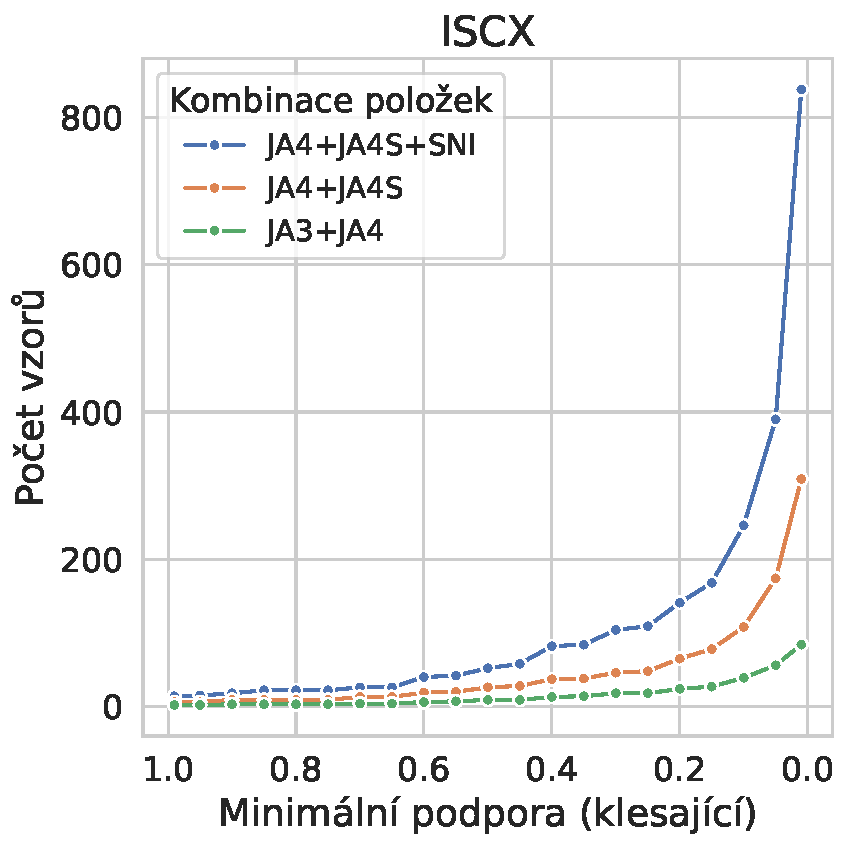
\includegraphics[width=\linewidth]{obrazky-figures/exps/ex2-num_patterns-iscx.pdf}
		\caption{Počet vzorů v~závislosti na~podpoře pro~\texttt{iscx.csv}.}
		\label{fig:ex2-iscx-patterns}
	\end{minipage}%
	\hfill
	\begin{minipage}[t]{0.49\textwidth}
		\centering
		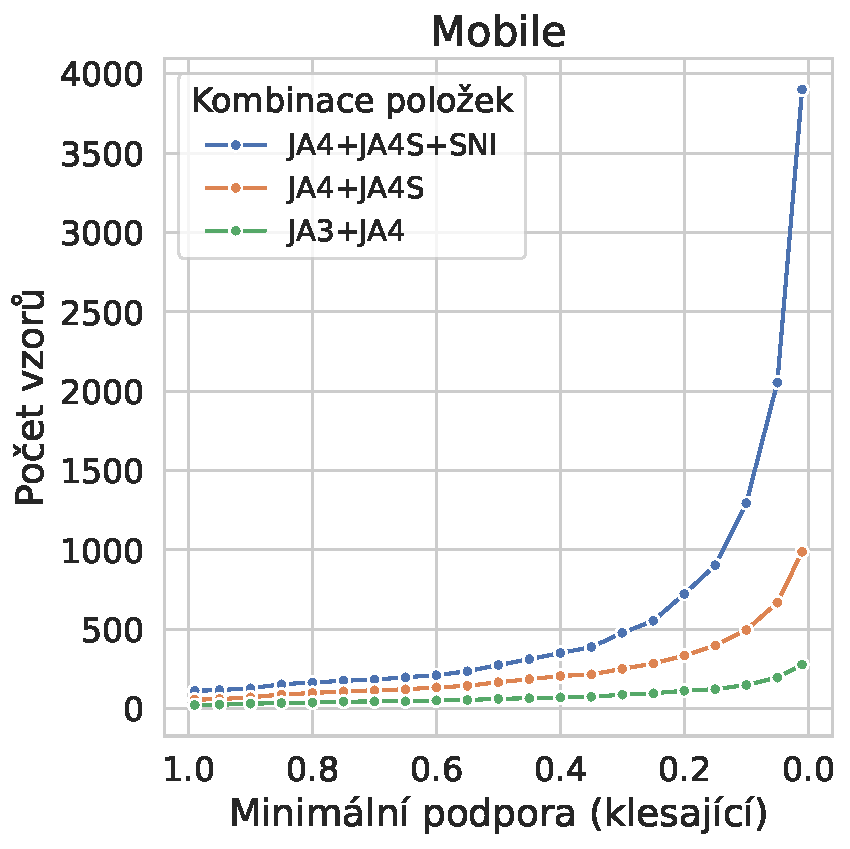
\includegraphics[width=\linewidth]{obrazky-figures/exps/ex2-num_patterns-mobile.pdf}
		\caption{Počet vzorů v~závislosti na~podpoře pro~\texttt{mobile\_desktop\_apps\_raw.csv}.}
		\label{fig:ex2-mobile-patterns}
	\end{minipage}
\end{figure}

Ostatní parametry pro~tento experiment byly nastaveny následovně: \textbf{šířka okna 15 spojení}, maximální \textbf{počet finálních kandidátů na~3}.

Je zřejmé, že volba minimální podpory přímo ovlivňuje počet identifikovaných vzorů v~rámci okolních spojení, jak ilustruje graf na~obrázku~\ref{fig:ex2-iscx-patterns} pro~datovou sadu \texttt{iscx.csv} a~graf na~obrázku~\ref{fig:ex2-mobile-patterns} pro~datovou sadu \texttt{mobile\_desktop\_apps\_raw.csv}. Lze rovněž očekávat, že celkový počet vzorů výrazně narůstá s~velikostí datové sady, což potvrzuje sada \texttt{mobile\_desktop\_apps\_raw.csv}, kde zaznamenaný počet vzorů \textbf{při minimální podpoře 0{,}01 dosahuje téměř 4000}. Naproti tomu u~sady \texttt{iscx.csv} celkový počet vzorů mírně \textbf{přesahuje hodnotu 800}.

V obou datových sadách je přesnost identifikace při~nastavení minimální podpory v~intervalu $(0{,}30; 0{,}99\rangle$ poměrně nízká a~roste s~klesající hodnotou podpory. V~nejlepších případech dosahuje maximálně hodnoty 0{,}7. Při~podpoře \textbf{nižší než 0{,}3} vykazují obě datové sady výrazně lepší úroveň identifikace.
\begin{figure}[H]
	\centering
	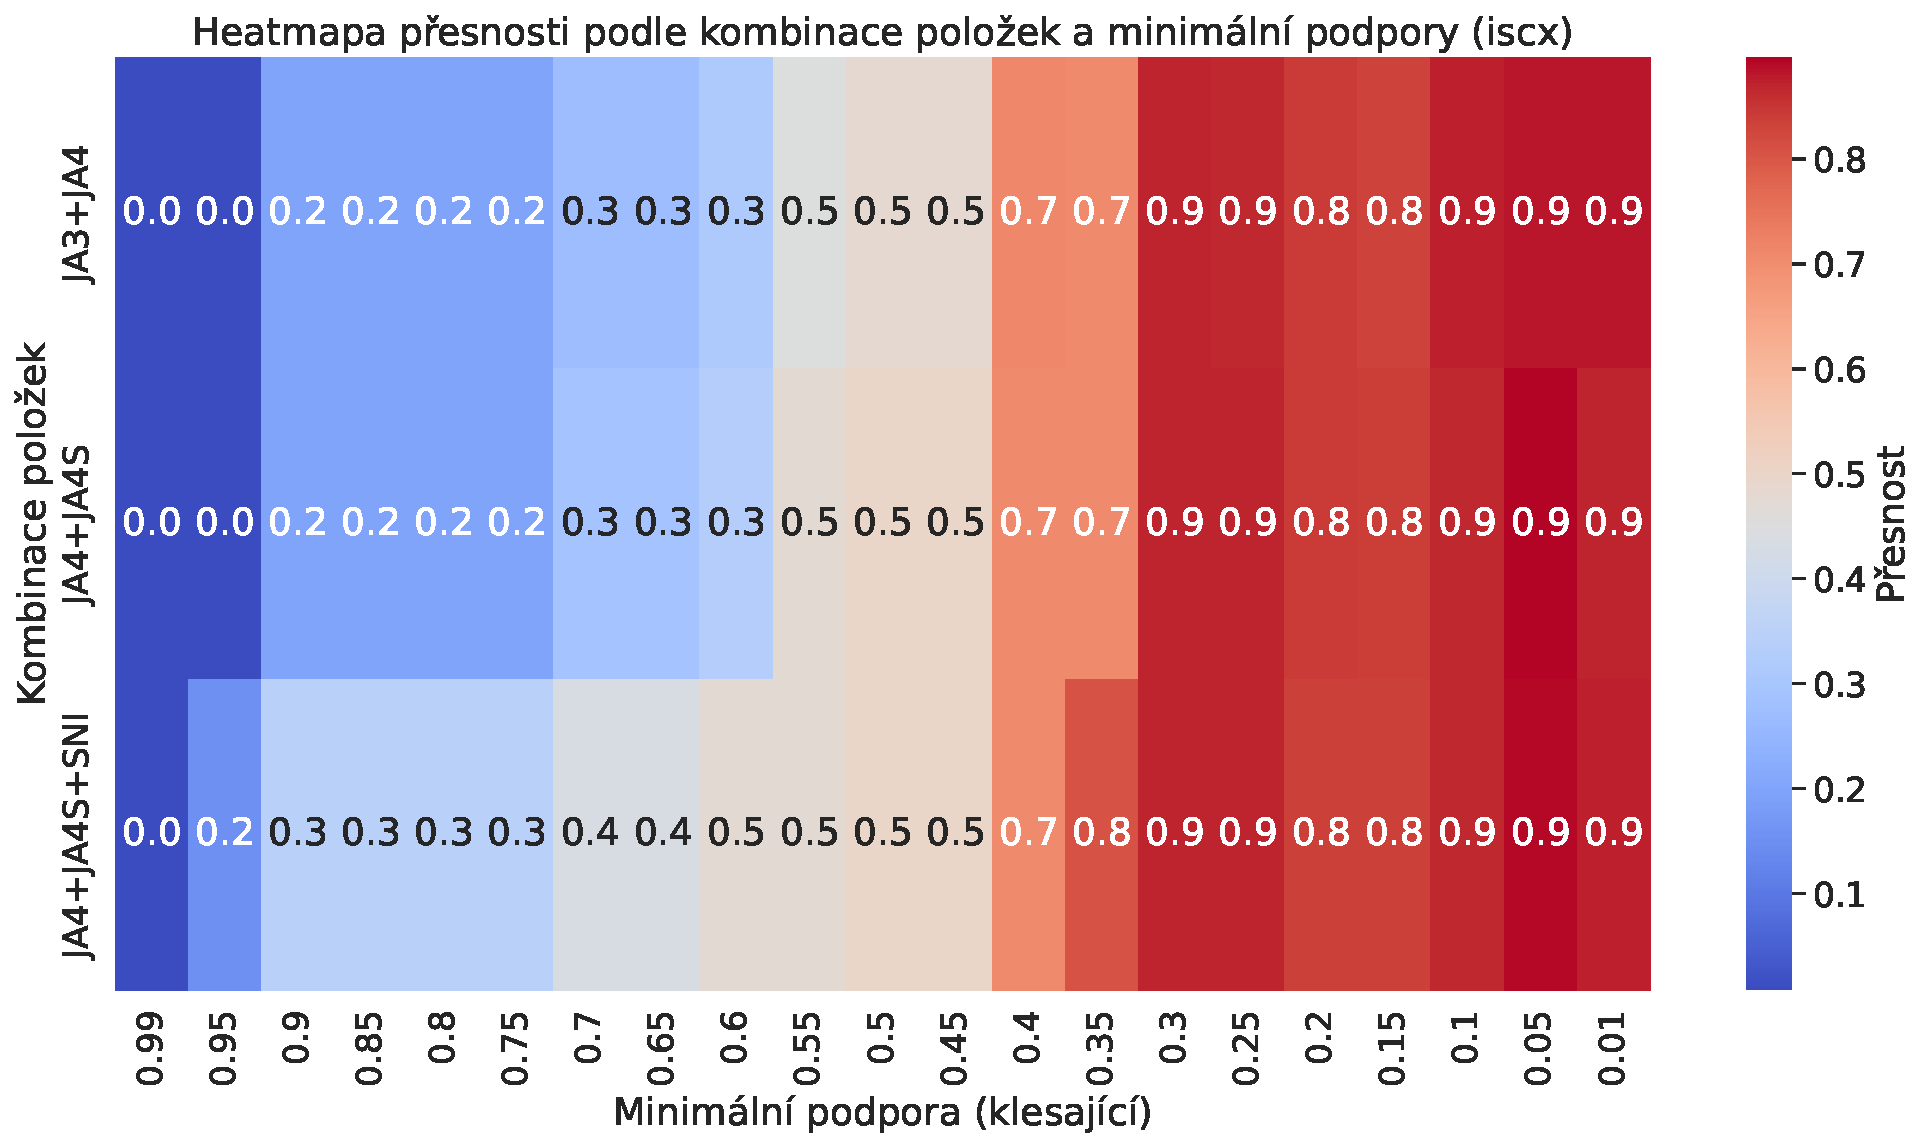
\includegraphics[width=\textwidth]{obrazky-figures/exps/ex2-iscx-heatmap.pdf}
	\caption{Heatmapa znázorňuje testované kombinace položek pro~algoritmus \textit{Apriori} v~závislosti na~volbě minimální podpory a~dosažené přesnosti pro~datovou sadu \texttt{iscx.csv}, při~použití metody \textit{JA4+JA4S+SNI} pro~nalezení počáteční kandidátní množiny.}
	\label{fig:ex2-iscx-heatmap}
\end{figure}
U datové sady \texttt{iscx.csv} (viz.obr.~\ref{fig:ex2-iscx-heatmap}) lze pozorovat, že všechny testované kombinace dosahují nejvyšší míry identifikace při~hodnotách podpory 0{,}3, 0{,}25 a~0{,}05. Druhá datová sada \texttt{mobile\_desktop\_apps\_raw.csv} (viz.obr.~\ref{fig:ex2-mobile-heatmap}) si od~podpory 0{,}3 udržuje podobnou úroveň přesnosti napříč všemi kombinacemi. Nejlepších výsledků však dosahuje kombinace \textit{JA4+JA4S+SNI} při~hodnotách podpory 0{,}25, 0{,}2, 0{,}05 a~0{,}01. Přesnější identifikace od~těchto hodnot je pravděpodobně způsobena tím, že při~hodnotě 0{,}26 již všechny aplikace mají minimálně jeden vzor.

Experiment byl rovněž proveden s~využitím metody \textit{JA4} pro~generování kandidátní množiny určené k~následné úpravě. Přestože se kombinace \textit{JA4+JA4S+SNI} dosud jeví jako nejvhodnější varianta, výsledky ukazují, že samotný otisk \textit{JA4} zatím nedosahuje požadované úrovně přesnosti. Kompletní výsledky experimentu jsou uvedeny v~příloze~\ref{sec:appendix:ex2}.

\begin{figure}[H]
	\centering
	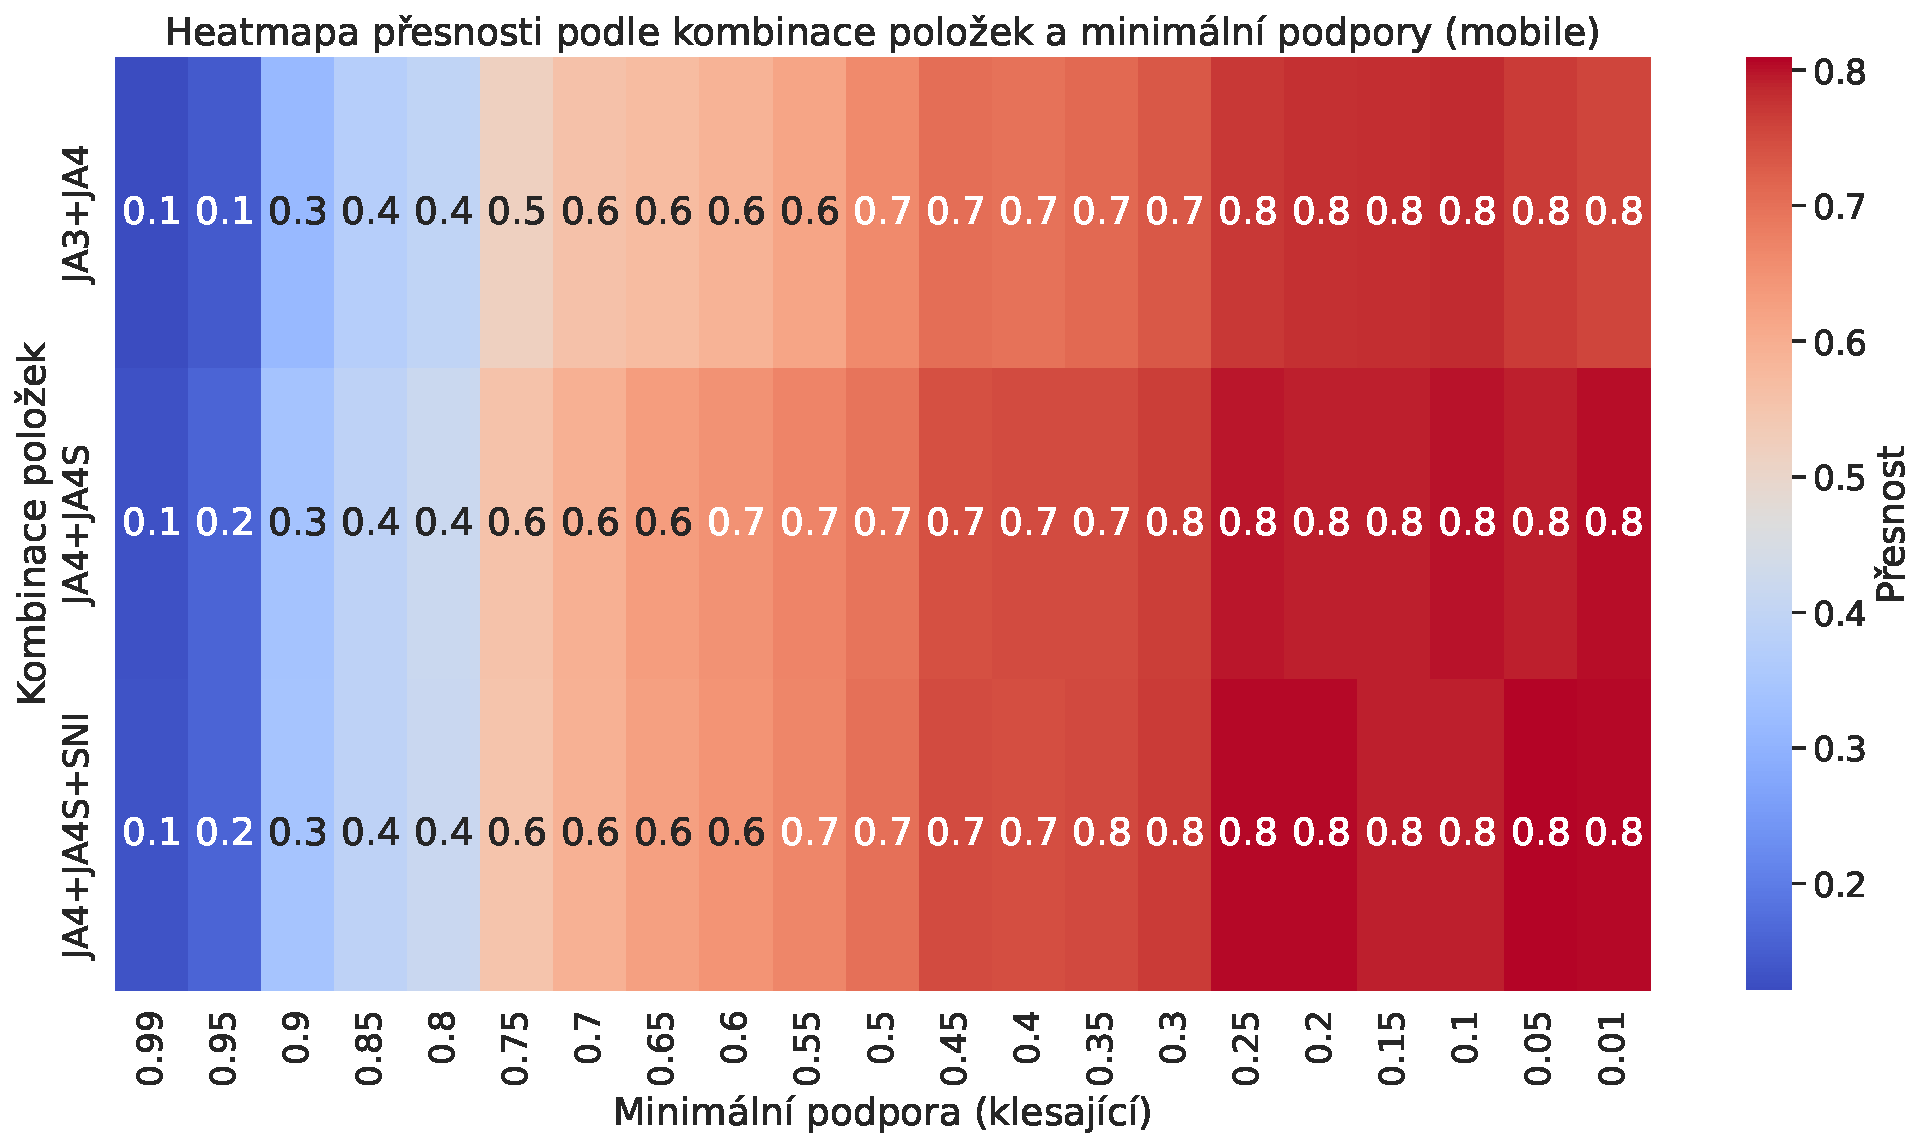
\includegraphics[width=\textwidth]{obrazky-figures/exps/ex2-mobile-heatmap.pdf}
	\caption{Heatmapa zobrazující testované kombinace položek pro~algoritmus \textit{Apriori} v~závislosti na~volbě minimální podpory a~dosažené přesnosti pro~datovou sadu \texttt{mobile desktop apps raw.csv}, při~použití metody \textit{JA4+JA4S+SNI} pro~nalezení počáteční kandidátní množiny.}
	\label{fig:ex2-mobile-heatmap}
\end{figure}

\begin{figure}[H]
	\centering
	\begin{minipage}[t]{0.49\textwidth}
		\centering
		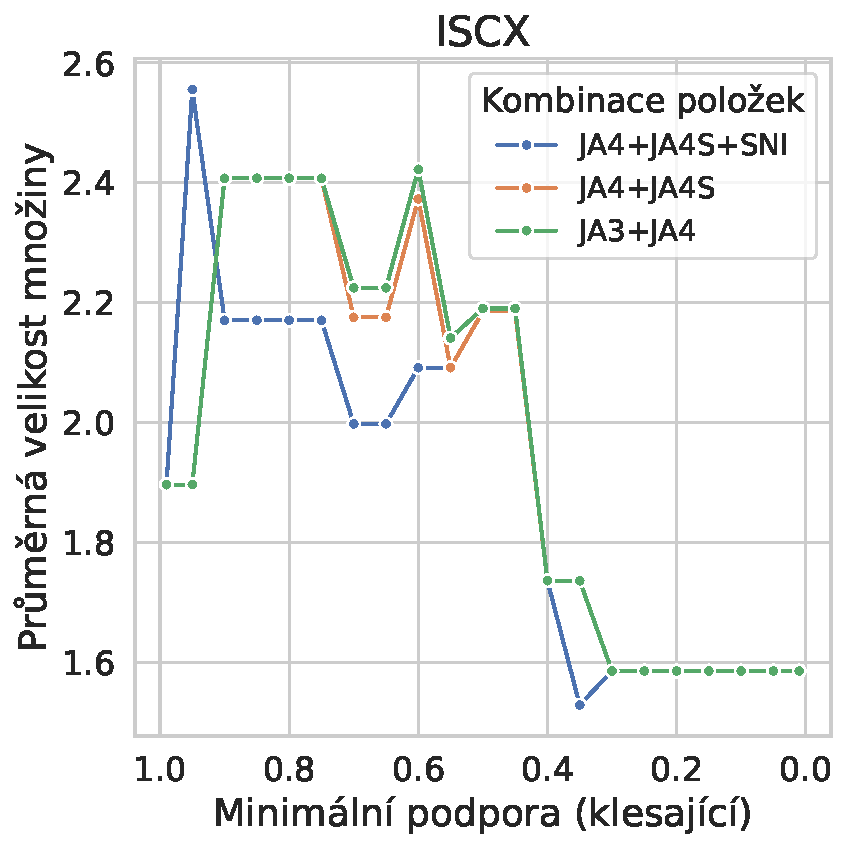
\includegraphics[width=\linewidth]{obrazky-figures/exps/ex2-candidates_len-iscx.pdf}
		\caption{Průměrná velikost finální kandidátní množiny v~závislosti na~podpoře pro~\texttt{iscx csv}.}
		\label{fig:ex2-iscx-candidates}
	\end{minipage}%
	\hfill
	\begin{minipage}[t]{0.49\textwidth}
		\centering
		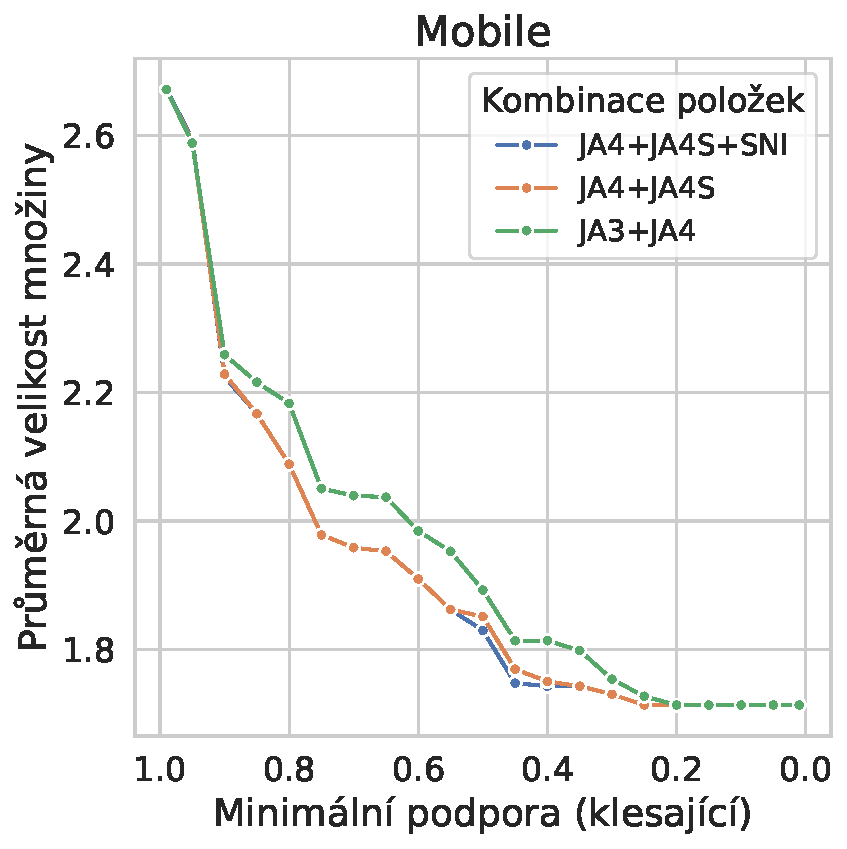
\includegraphics[width=\linewidth]{obrazky-figures/exps/ex2-candidates_len-mobile.pdf}
		\caption{Průměrná velikost finální kandidátní množiny v~závislosti na~podpoře pro~\texttt{mobile desktop apps raw.csv}.}
		\label{fig:ex2-mobile-candidates}
	\end{minipage}
\end{figure}

Průměrná velikost finální kandidátní množiny klesá se snižující se minimální podporou u~obou datových sad. U~datové sady \texttt{iscx.csv} (viz.~graf na~Obrázku~\ref{fig:ex2-iscx-candidates}) jsou rozdíly mezi~jednotlivými kombinacemi výraznější než u~sady \texttt{mobile\_desktop\_apps\_raw.csv} (viz.~graf na~Obrázku~\ref{fig:ex2-mobile-candidates}). Nicméně při~hodnotách podpory 0{,}2 a~nižších konvergují všechny kombinace k~téměř stejné, nejnižší zaznamenané hodnotě (v případě \texttt{iscx.csv} k~druhé nejnižší zaznamenané hodnotě).

V této fázi z~experimentu vyplývá, že nejlepší výsledky v~rámci nastavení minimální podpory se pohybují kolem \textbf{hodnot 0{,}2, 0{,}25 , 0{,}05 nebo 0{,}01}. S~ohledem na~počet vytěžených vzorů se však hodnoty \textbf{0{,}2 a~0{,}25 jeví jako ideální volba} pro~budoucí experimenty. Nabízí totiž srovnatelnou úroveň identifikace jako nižší hodnoty (například 0{,}05), avšak \textbf{s~výrazně menším počtem vzorů}, což snižuje výpočetní náročnost i~složitost následného zpracování.

\subsection{Velikost a~počet vzorů na~aplikaci}
\label{ex-filters}
Tato část představuje druhou fázi experimentu, která se zaměřuje na~analýzu počtu a~délky vzorů přiřazených jednotlivým aplikacím. Cílem je detailněji prozkoumat získané vzory a~jejich vlastnosti s~ohledem na~optimalizaci následné identifikace. Analyzovány jsou všechny vzory získané při~použití hodnot minimální podpory, které se v~předchozí fázi ukázaly jako nejefektivnější: \textbf{0{,}01}, \textbf{0{,}05}, \textbf{0{,}2} a~\textbf{0{,}25}. Ostatní parametry zůstávají beze změny – konkrétně se jedná o~šířku okna na~\textbf{15 spojení}, omezení maximálního počtu finálních \textbf{kandidátů na~3} a~využití metody \textit{JA4+JA4S+SNI} jak pro~\textbf{generování počáteční kandidátní množiny}, tak pro~\textbf{nalezení frekventovaných vzorů}. Vzory jsou dále zkoumány za~účelem jejich selekce -- tedy filtrování na~základě jejich počtu a~délky, s~cílem snížit výpočetní náročnost a~zároveň zvýšit efektivitu procesu identifikace.

\begin{figure}[H]
	\centering
	\begin{minipage}[t]{0.49\textwidth}
		\centering
		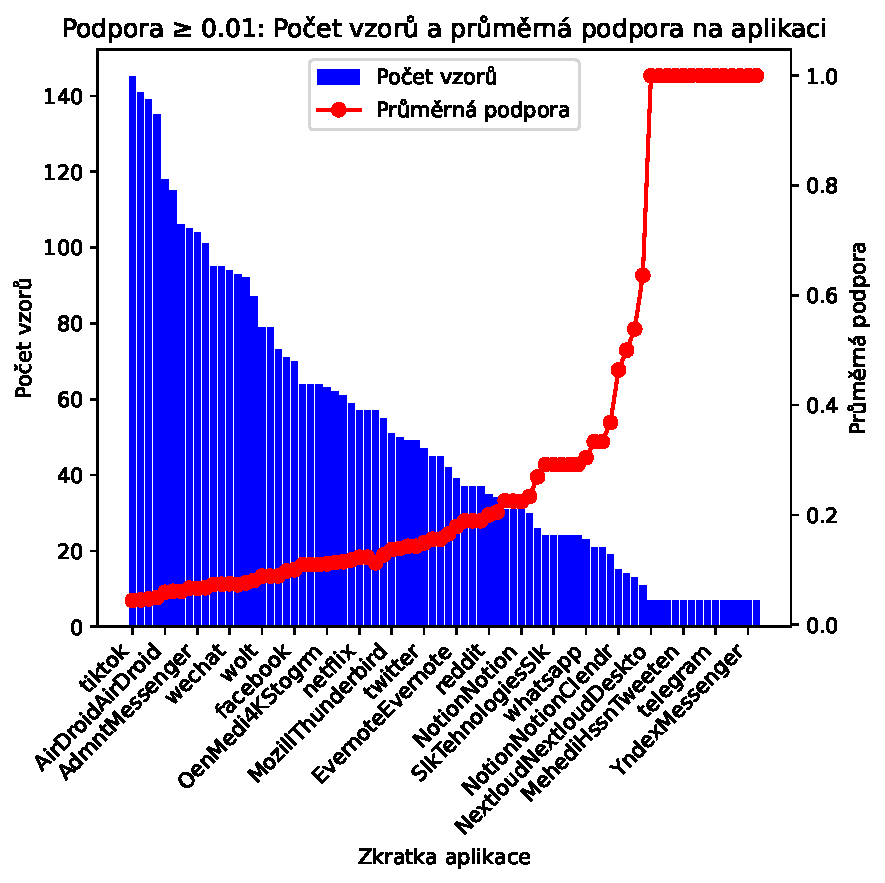
\includegraphics[width=\linewidth]{obrazky-figures/exps/patterns_support_0.01_mobile.pdf}
		\caption{Počet vzorů a~průměrná podpora na~aplikaci -- \texttt{mobile desktop apps.csv}}
		\label{fig:graph-num-vs-apps-mobile-001}
	\end{minipage}
	\hfill
	\begin{minipage}[t]{0.49\textwidth}
		\centering
		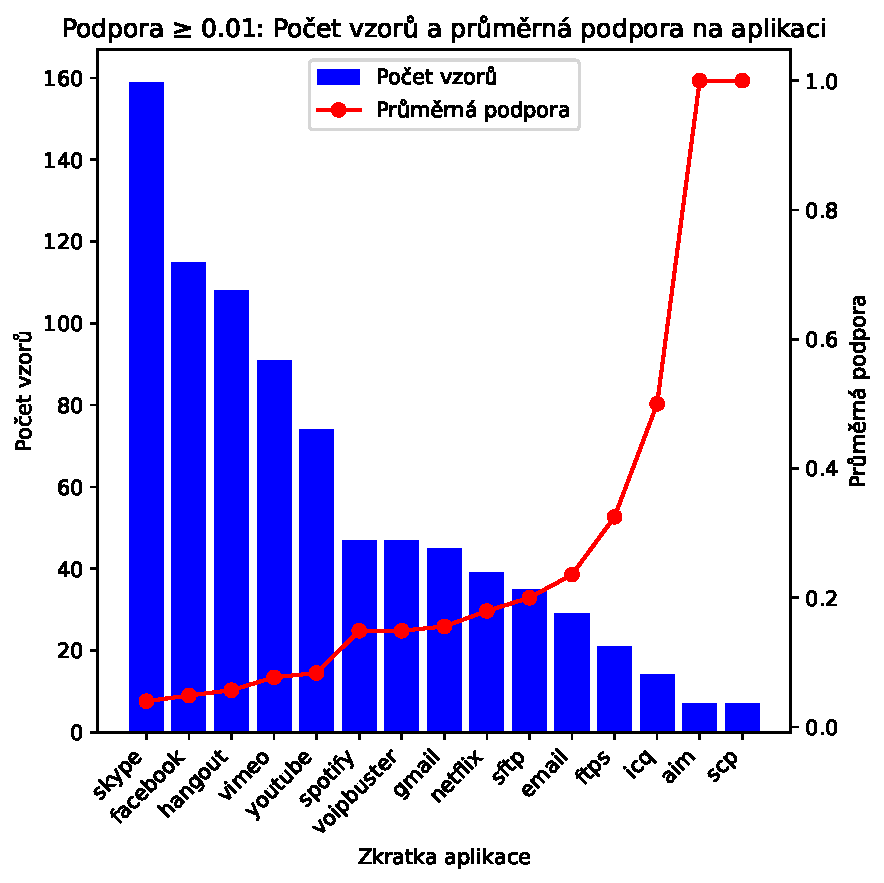
\includegraphics[width=\linewidth]{obrazky-figures/exps/patterns_support_0.01_iscx.pdf}
		\caption{Počet vzorů a~jejich průměrná podpora na~aplikaci -- \texttt{iscx.csv}}
		\label{fig:graph-num-vs-apps-iscx-001}
	\end{minipage}
\end{figure}


Graf na~obrázku\footnote{U všech následujících grafů jsou z~důvodu přehlednosti zobrazeny popisky pouze pro~každou čtvrtou aplikaci z~datové sady \texttt{mobile\_desktop\_apps\_raw.csv}.}~\ref{fig:graph-num-vs-apps-mobile-001} znázorňuje počet získaných vzorů při~prahu minimální podpory 0{,}01 pro~každou aplikaci z~datové sady \texttt{mobile\_desktop\_apps\_raw.csv}. Je patrné, že mezi~aplikací s~nejnižším a~nejvyšším počtem vzorů je výrazný rozdíl — konkrétně až \textbf{130 vzorů}. V~grafu je rovněž vyznačena průměrná podpora vytěžených vzorů pro~jednotlivé aplikace, přičemž lze pozorovat, že některé aplikace obsahují vzory s~podporou rovnou 1{,}0. To znamená, že se tyto vzory vyskytují ve všech jejich instancích. Tento jev lze pravděpodobně přičíst malému testovacímu vzorku daných aplikací.

Obdobně je v~grafu na~obrázku~\ref{fig:graph-num-vs-apps-iscx-001} znázorněn průměrný počet vzorů a~jejich podpora pro~jednotlivé aplikace v~datové sadě \texttt{iscx.csv}. Také v~tomto případě je patrný výrazný rozdíl v~počtu vzorů mezi~jednotlivými aplikacemi, který dosahuje až \textbf{152 vzorů}. Kompletní přehled, počtu vzorů a~jejich průměrné podpory pro~dříve zmíněné hodnoty minimální podpory, je uveden v Příloze~\ref{sec:appendix:ex2}.

Kvůli tomuto výraznému nepoměru v~počtu vzorů napříč aplikacemi bylo nutné při~výpočtu podobnosti zohlednit nejen samotnou přítomnost vzorů, ale i~jejich podporu (frekvenci výskytu v~rámci dané aplikace) a~unikátnost (míru výskytu napříč všemi aplikacemi), jak je popsáno v~podsekci~\ref{subsec:klicove}. 

Alternativním přístupem je normalizace počtu vzorů mezi~aplikacemi, například filtrováním na~přibližně stejný počet vzorů podle stanovených kritérií (např. délka či podpora). Tento krok by mohl předejít zkreslení, které vzniká v~případech, kdy některé aplikace disponují nepřiměřeně vysokým počtem vzorů s~nízkou podporou, zatímco jiné obsahují pouze několik málo specifických a~silně reprezentativních vzorů. Při~vyšší minimální podpoře již není rozdíl v~počtu získaných vzorů mezi~aplikacemi tak markantní. Nicméně identifikace při~stejném počtu informativně rovnocenných vzorů by měla teoreticky být vyváženější a~tím pádem přesnější.

Z tohoto důvodu je provedena analýza délky vzorů pro~jednotlivé aplikace. Kratší vzory mají tendenci vést k~častějším, ale obecnějším identifikacím, zatímco delší vzory mohou poskytnout specifičtější identifikaci, avšak s~nižší frekvencí výskytu.

\begin{figure}[H]
	\centering
	\begin{minipage}[t]{0.5\textwidth}
		\centering
		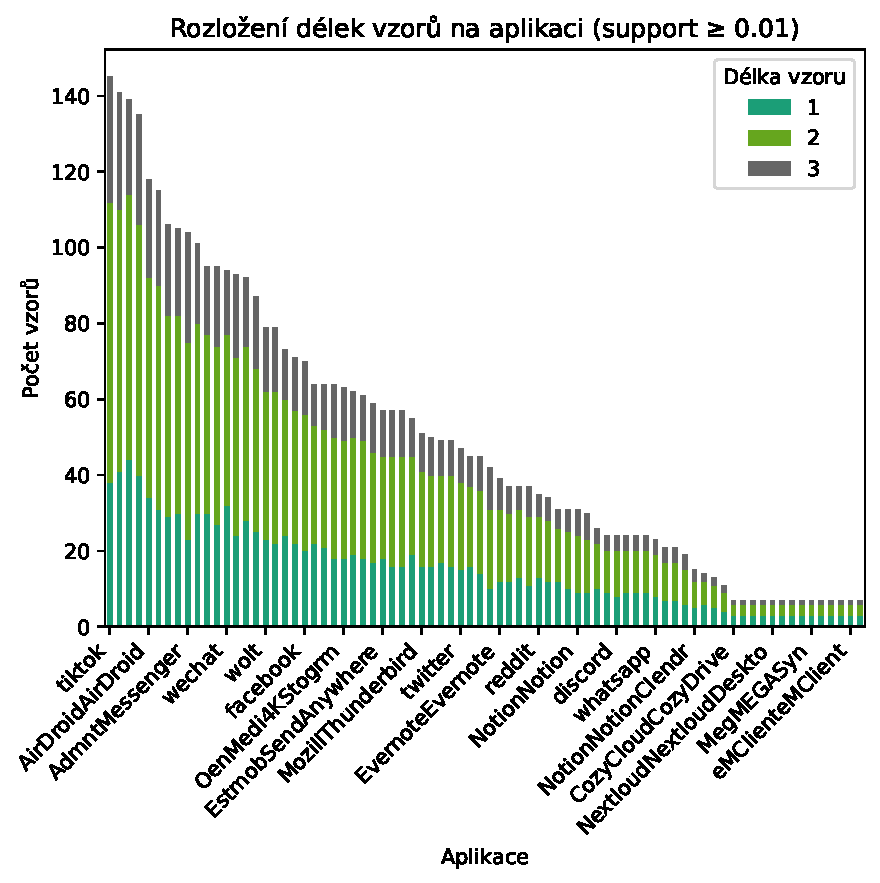
\includegraphics[width=\linewidth]{obrazky-figures/exps/pattern_lengths_0.01_mobile.pdf}
		\caption{Rozložení délek vzorů na~aplikaci při~minimální podpoře 0{,}01 pro~\texttt{mobile desktop apps raw.csv}}
		\label{fig:ex2-mobile-patterns-len}
	\end{minipage}
	\hfill
	\begin{minipage}[t]{0.49\textwidth}
		\centering
		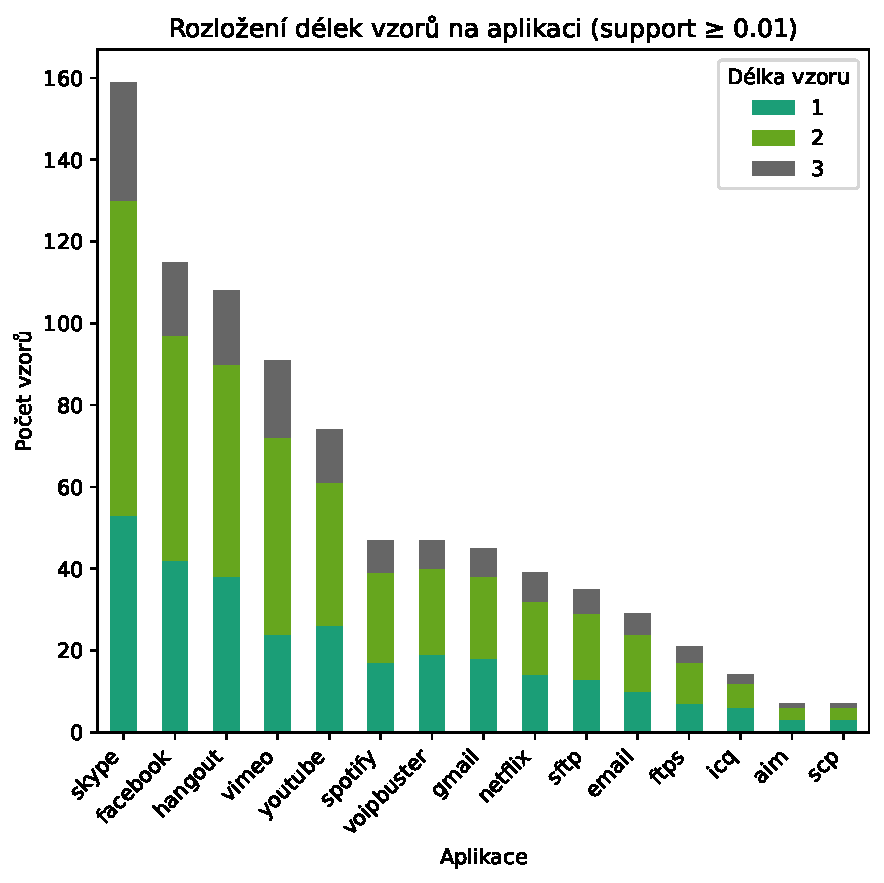
\includegraphics[width=\linewidth]{obrazky-figures/exps/pattern_lengths_0.01_iscx.pdf}
		\caption{Rozložení délek vzorů na~aplikaci při~minimální podpoře 0{,}01 pro~\texttt{iscx.csv}}
		\label{fig:ex2-iscx-patterns-len}
	\end{minipage}
\end{figure}

Grafy na~obrázcích~\ref{fig:ex2-mobile-patterns-len} a~\ref{fig:ex2-iscx-patterns-len} znázorňují rozložení délek získaných vzorů aplikací při~minimální podpoře 0.01 pro~datové sady \texttt{mobile\_desktop\_apps\_raw.csv} a~\texttt{iscx.csv}. V~obou případech převažují vzory o~délce 1 a~2. Jak bylo již uvedeno, vzory o~délce 3 jsou méně časté, ale mohou poskytnout informativně cennější hodnotu díky své specifičnosti. 

Viz.grafy na~obrázcích~\ref{fig:ex2-mobile-patterns-len-025} a~\ref{fig:ex2-iscx-patterns-len-025}, které znázorňují stejnou závislost při~změně hodnoty minimální podpory, která je nyní nastavena na~0.25. Při~této podpoře jsou častější obecnější vzory o~délce 1, zatímco vzory o~délce 3 jsou zde zastoupeny ve výrazně menším počtu, v~některých případech již vůbec. Hodnota podpory 0.26 představuje hranici pro~oba datové soubory. Při~této hodnotě již pro~některé aplikace nebyly nalezeny žádné vzory. Konkrétně se jedná o~aplikaci \textit{facebook} v~datové sadě \texttt{iscx.csv} a~\textit{alipay} v~sadě \texttt{mobile\_desktop\_apps\_raw.csv}. Tento jev je patrný i~v~grafech, kde je zřetelný pokles počtu vzorů, přičemž u~těchto aplikací, jako je \textit{facebook} a~\textit{alipay}, se v~tomto rozmezí nachází pouze jeden vzor.

\begin{figure}[H]
	\centering
	\begin{minipage}[t]{0.5\textwidth}
		\centering
		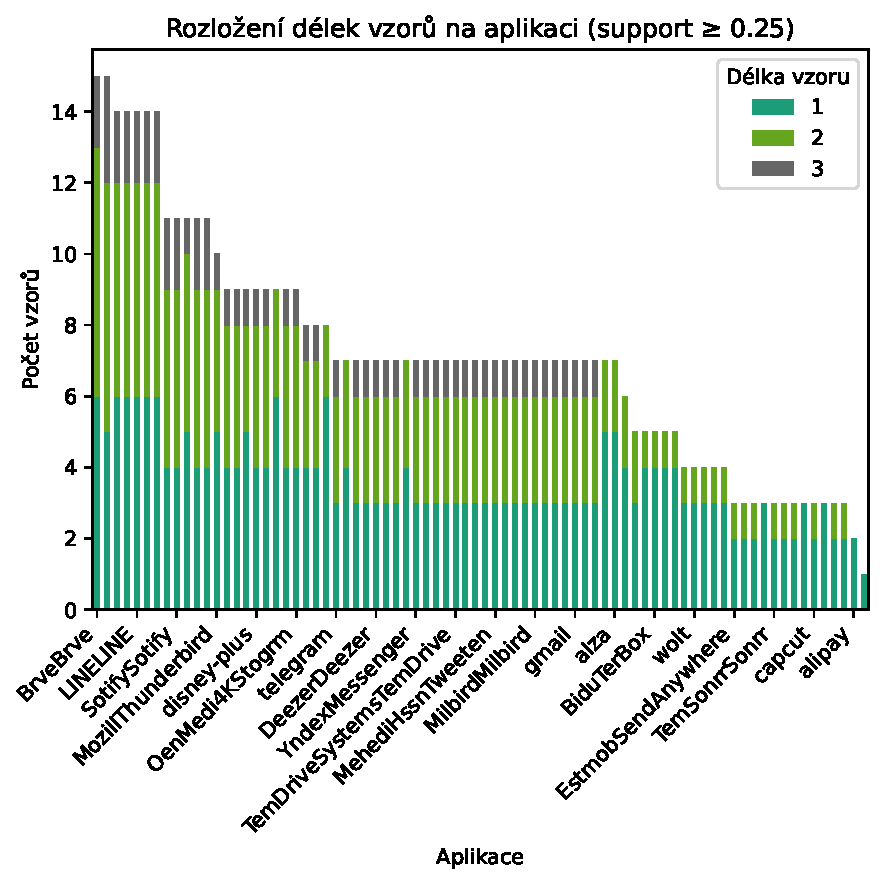
\includegraphics[width=\linewidth]{obrazky-figures/exps/pattern_lengths_0.25_mobile.pdf}
		\caption{Rozložení délek vzorů na~aplikaci při~minimální podpoře 0{,}25 pro~\texttt{mobile desktop apps raw.csv}}
		\label{fig:ex2-mobile-patterns-len-025}
	\end{minipage}
	\hfill
	\begin{minipage}[t]{0.49\textwidth}
		\centering
		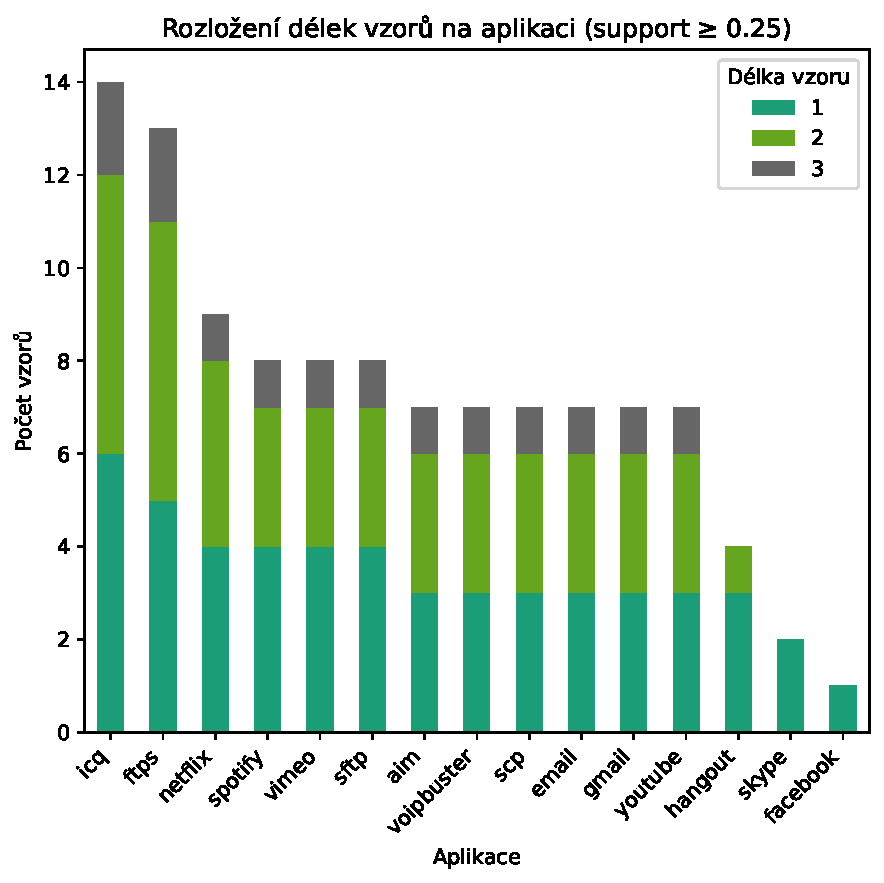
\includegraphics[width=\linewidth]{obrazky-figures/exps/pattern_lengths_0.25_iscx.pdf}
		\caption{Rozložení délek vzorů na~aplikaci při~minimální podpoře 0{,}25 pro~\texttt{iscx.csv}}
		\label{fig:ex2-iscx-patterns-len-025}
	\end{minipage}
\end{figure}

Vzory byly filtrovány dle délky, přičemž v~rámci každé délkové skupiny byly seřazeny podle podpory. Byla vytvořena sada filtrů na~základě předchozí analýzy počtu a~délky vzorů. Následně bylo z~každé množiny vybráno $N$ vzorů podle zvoleného filtru.

Různé varianty filtrů byly otestovány pro~čtyři hodnoty minimální podpory: \textbf{0{,}01}, \textbf{0{,}05}, \textbf{0{,}2} a~\textbf{0{,}25}. Jako vstupní množina pro~algoritmus \textit{Apriori} byly konzistentně použity otisky \textit{JA4}, \textit{JA4S} a~atribut spojení \textit{SNI}. Cílem této fáze bylo porovnat přesnost výsledné kandidátní množiny vůči referenčnímu stavu bez~jakékoli filtrace (viz~Obrázky~\ref{fig:ex2-iscx-heatmap} a~\ref{fig:ex2-mobile-heatmap}).

Následující tabulky shrnují nejzajímavější výsledky jednotlivých filtrů z~hlediska identifikační přesnosti a~počtu použitých vzorů. \textbf{Kombinace} označují konkrétní otisky a~atributy spojení použitých pro~generování počáteční kandidátní množiny. \textbf{Podpora} udává hodnotu minimální podpory použitou při~těžbě vzorů. \textbf{Filtr} reprezentuje způsob filtrování vzorů ve formátu \(len(n)Xm\), kde \(len(n)\) označuje délku vzoru a~\(Xm\) specifikuje počet takových vzorů. Pokud je parametr \(Xm\) vynechán, znamená to, že jsou použity všechny vzory dané délky. Dále byly testovány i~kombinace více filtrů, které jsou označeny symbolem \(+\). 

\begin{table}[H]
	\centering
	\begin{tabular}{lrlll}
		\toprule
		\multicolumn{5}{c}{\texttt{iscx.csv}}  \\
		\midrule
		Kombinace    & Podpora & Filtr              & Přesnost & Prům. délka množiny \\
		\midrule
		JA4          & 0.01    & len(1)x5+len(3)x10 & 0.91      & 2.128395                    \\
		JA4          & 0.01    & len(2)x5           & 0.91      & 2.128395                    \\
		JA4          & 0.01    & len(3)             & 0.91      & 2.128395                    \\
		JA4+JA4S+SNI & 0.05    & len(3)x10          & 0.89      & 1.585185                    \\
		JA4+JA4S+SNI & 0.05    & len(3)             & 0.89      & 1.585185                    \\
		JA4+JA4S+SNI & 0.05    & len(3)x5           & 0.89      & 1.585185                    \\
		\bottomrule
	\end{tabular}
	\caption{Top 3 výsledky, pro~každou kombinaci generující počáteční množinu,  podle přesnosti s~aplikací filtrů  u~datové sady \texttt{iscx.csv}}
	\label{tab:top3-iscx}
\end{table}

V tabulce~\ref{tab:top3-iscx} jsou uvedeny výsledky přesnosti jednotlivých filtrů pro~datovou sadu \texttt{iscx.csv}. Kombinace \textit{JA4}, která vytváří počáteční množinu, vykazuje velmi mírné zlepšení u~výše zmíněných filtrů, přičemž průměrná velikost kandidátní množiny zůstává nezměněna. Druhá kombinace \textit{JA4+JA4S+SNI} nevykazuje žádné zlepšení.

\begin{table}[H]
	\centering
	\begin{tabular}{lrlll}
		\toprule
		\multicolumn{5}{c}{\texttt{mobile\_desktop\_apps\_raw.csv}}  \\
		\midrule
		Kombinace    & Podpora & Filtr              & Přesnost & Prům. délka množiny \\
		\midrule
		JA4+JA4S+SNI & 0.01    & len(1)x2+len(3)x2  & 0.81      & 1.713638                    \\
		JA4+JA4S+SNI & 0.05    & len(1)x2+len(3)x2  & 0.81      & 1.713638                    \\
		JA4+JA4S+SNI & 0.20    & len(1)x5+len(2)x10 & 0.81      & 1.713638                    \\
		JA4          & 0.01    & len(2)x5+len(3)x10 & 0.80      & 2.790678                    \\
		JA4          & 0.01    & len(2)x5+len(3)x5  & 0.78      & 2.790678                    \\
		JA4          & 0.01    & len(3)             & 0.78      & 2.790678                    \\
		\bottomrule
	\end{tabular}
	\caption{Top 3 výsledky, pro~každou kombinaci generující počáteční množinu,  podle přesnosti s~aplikací filtrů  u~datové sady \texttt{mobile desktop apps raw.csv}}
	\label{tab:top3-mobile}
\end{table} 

Datová sada \texttt{mobile\_desktop\_apps\_raw.csv} při~použití filtrů taktéž nevykazuje žádné významné zlepšení v~přesnosti identifikace ani ve zmenšení velikosti kandidátní množiny (viz. Tabulka~\ref{tab:top3-mobile}). Přestože se mohou výsledky jevit jako málo přínosné, z~pohledu optimalizace procesu identifikace přinášejí určitý benefit -- zejména v~podobě redukce počtu vzorů, které je nutné porovnávat, a~jejich částečné normalizace napříč aplikacemi.

Z tabulek~\ref{tab:top3-mobile} a~\ref{tab:top3-iscx} je patrné, že nejlepších výsledků přesnosti je dosahováno při~různých kombinacích filtrů a~parametrů pro~každou z~datových sad. Zatímco pro~\texttt{iscx.csv} se jako nejefektivnější jeví selekce zaměřená na~delší vzory (např. \texttt{len(3)} nebo \texttt{len(2)x5}) a~nižší hodnoty podpory, u~datové sady \texttt{mobile\_desktop\_apps\_raw.csv} dosahují srovnatelné přesnosti filtry kombinující obecné a~specifické vzory (např. \texttt{len(1)x2+len(3)x2}) i~při~vyšších hodnotách podpory.

Použitím nižší hodnoty minimální podpory je zároveň možné zachytit i~méně časté, ale informačně hodnotnější vzory. Ty mohou být klíčové pro~přesnější rozlišení mezi~jednotlivými spojeními, která nelze efektivně identifikovat pomocí obecnějších vzorů vznikajících při~vyšších prahových hodnotách. Aplikace filtrů pak umožňuje tyto specifické vzory v~databázi ponechat, čímž přispívá k~vyváženějšímu kompromisu mezi~výpočetní efektivitou a~identifikační schopností.

\begin{wrapfigure}{r}{0.5\textwidth}
	\centering
	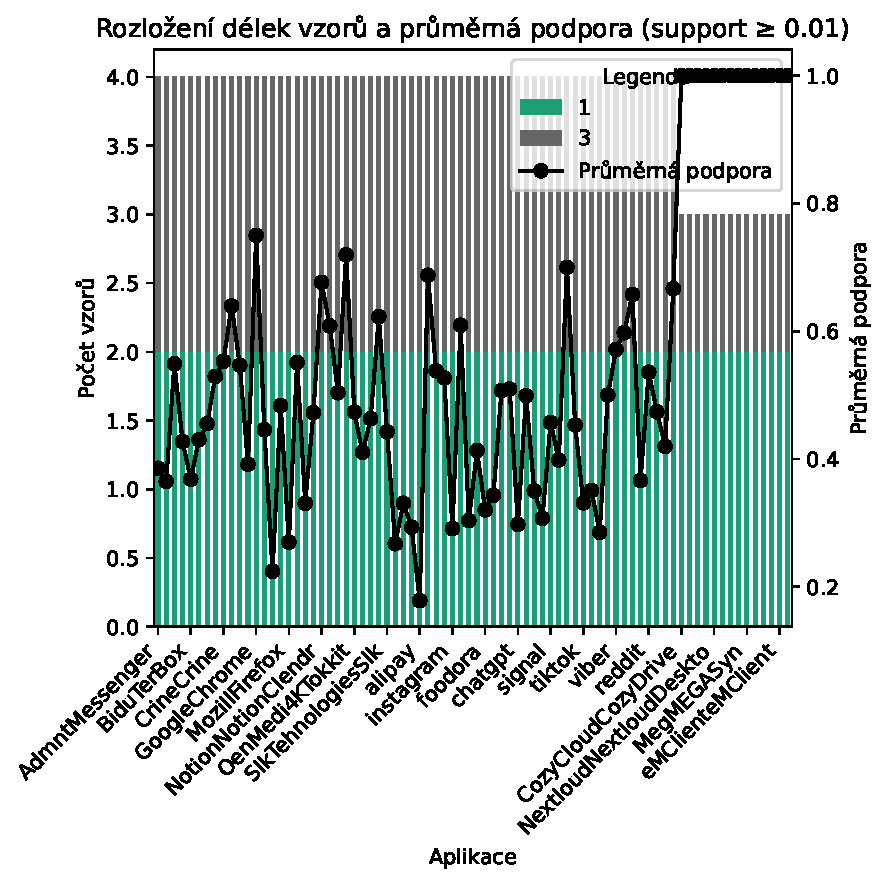
\includegraphics[width=0.49\textwidth]{obrazky-figures/exps/pattern_lengths_filtered_0.01_mobile.pdf}
	\caption{Rozložení délek vzorů a~průměrná podpora po~aplikaci filtrace \texttt{len(1)x2 a~len(3)x2} pro~\texttt{mobile desktop apps raw.csv} s~minimální podporou 0{,}01}
	\label{fig:pattern_lengths-filtered-mobile}
\end{wrapfigure}

Graf na~obrázku~\ref{fig:pattern_lengths-filtered-mobile} znázorňuje aplikovanou selekci pomocí filtru \texttt{len(1)x2 + len(3)x2} a~minimální podpory \textbf{0{,}01} pro~datovou sadu \texttt{mobile\_desktop\_apps\_raw.csv}. Toto nastavení dosahuje přesnosti \textbf{0{,}8129} při~průměrné velikosti finální kandidátní množiny \textbf{1{,}7}. Modus i~medián této velikosti jsou rovny \textbf{1}. Většina aplikací si uchovává právě dva vzory délky 1 a~dva vzory délky 3. U~menšiny aplikací však nebyly nalezeny dva vzory délky 3, ale pouze jeden.

Tento experiment ukázal, že selektivní filtrování vzorů může vést k~efektivnější (méně náročnější) identifikaci, přičemž negativní dopad na~přesnost se projevuje až při~použití vyšších hodnot minimální podpory. Při~nízké podpoře a~vhodně zvolených filtrech je tento dopad téměř zanedbatelný (viz~\ref{sec:appendix:ex2}). 

Přestože se nejedná o~univerzálně aplikovatelné řešení, výsledky potvrzují, že pro~různé datové sady je možné nalézt vhodnou kombinaci parametrů (podpora, délka, počet vzorů), která zajistí optimální rovnováhu mezi~výpočetní náročností a~kvalitou identifikace. Kompletní výsledky se všemi použitými filtry pro~obě datové sady a~obě kombinace jsou uvedeny v~příloze~\ref{chp:appendix-experiments}.

\section{Šířka okna určující okolí spojení}
\label{sec:ex-window}
Kontext každého identifikovaného spojení je určen velikostí posuvného okna, jak je popsáno v~podsekci~\ref{subsec:klicove}. Ve většině případů se ve středu tohoto okna nachází právě identifikované spojení, zatímco jeho okolí může tvořit buď další spojení stejné aplikace (například v~rámci jednoho spuštění), nebo spojení patřící jiným aplikacím. Vzhledem k~náhodnému uspořádání testovací množiny může dojít k~tomu, že do~okna spadají i~nesouvisející spojení, což způsobuje informační šum a~může negativně ovlivnit kvalitu identifikace.

Cílem tohoto experimentu je určit optimální velikost okna, která zachytí dostatek relevantního kontextu pro~přesnou identifikaci, aniž by zahrnovala rušivá data z~jiných aplikací. 

V~rámci experimentu byly parametry nastaveny na~použití metody \textbf{\textit{JA4+JA4S+SNI}} jak pro~generování \textbf{počáteční} kandidátní množiny, tak i~pro~nalezení \textbf{častých vzorů}. \textbf{Minimální podpora} byla nastavena na~\textbf{0{,}01} a~byla využita selekce filtrů z~předchozího experimentu. Maximální počet kandidátů byl zvolen na~\textbf{3}. Testovány byly různé hodnoty šířky kontextového okna (vždy liché číslo, aby byl kontext z~obou stran vyvážen), konkrétně \textbf{3, 5, 7, 9, 11, 21} a~\textbf{31}.
V~tabulce~\ref{tab:used_filters-ex4} jsou uvedeny jednotlivé použité filtry, které byly zvoleny na~základě nejvyšší dosažené přesnosti v~předchozím experimentu.

\begin{table}[H]
	\centering
	\begin{tabular}{lll}
		\toprule
		Kombinace    & \texttt{mobile\_desktop\_apps\_raw.csv} & \texttt{iscx.csv}  \\
		\midrule
		JA4          & len(2)x5+len(3)x10                      & len(1)x5+len(3)x10 \\
		JA4+JA4S+SNI & len(1)x2+len(3)x2                       & len(3)x5           \\
		\bottomrule
	\end{tabular}
	\caption{Použité filtry pro~experiment}
	\label{tab:used_filters-ex4}
\end{table}
Následující tabulky uvádějí použitou šířku okna a~přesnost pro~daný otisk nebo kombinaci otisků, které byly použity pro~generování počáteční množiny. Nejvyšší dosažené přesnosti jsou v~tabulkách vyznačeny tučně.

\begin{table}[H]
	\centering
	\begin{minipage}{0.49\textwidth}
		\centering
		\begin{tabular}{cll}
			\toprule
			\multicolumn{3}{c}{\texttt{mobile\_desktop\_apps\_raw.csv}}  \\
			\midrule
			\multirow{2}{*}{Šířka okna} & \multicolumn{2}{l}{Přesnost při~kombinacích}\\
															    			
			            & JA4             & JA4+JA4S+SNI    \\
			\midrule
			\textbf{3}  & 0.7706          & \textbf{0.8157} \\
			5           & 0.8058          & 0.8133          \\
			7           & 0.8289          & 0.8133          \\
			\textbf{9}  & \textbf{0.8332} & 0.8131          \\
			\textbf{11} & 0.8280          & \textbf{0.8157} \\
			21          & 0.7644          & 0.8013          \\
			31          & 0.6877          & 0.7874          \\
			\bottomrule
		\end{tabular}
		\caption{Přesnost identifikace pro~různé velikosti okolí pro~datovou sadu \texttt{mobile desktop apps raw.csv}.}
		\label{tab:mobile_acc_vs_window}
										        
	\end{minipage}
	\hfill
	\begin{minipage}{0.49\textwidth}
												
		\centering
		\begin{tabular}{cll}
			\toprule
			\multicolumn{3}{c}{\texttt{iscx.csv}}  \\
			\midrule
			\multirow{2}{*}{Šířka okna} & \multicolumn{2}{l}{Přesnost při~kombinacích}\\
																		
			            & JA4             & JA4+JA4S+SNI    \\
			\midrule
			3           & 0.9111          & 0.8815          \\
			5           & 0.9012          & 0.8840          \\
			7           & 0.9012          & 0.8864          \\
			9           & 0.9062          & 0.8864          \\
			\textbf{11} & 0.9062          & \textbf{0.8914} \\
			\textbf{21} & \textbf{0.9185} & 0.8840          \\
			31          & 0.8864          & 0.8691          \\
			\bottomrule
		\end{tabular}
		\caption{Přesnost identifikace pro~různé velikosti okolí s~\textit{JA4+JA4S+SNI} a~\textit{JA4} pro~datovou sadu \texttt{iscx.csv}.}
		\label{tab:iscx_acc_vs_window}
										        
	\end{minipage}
\end{table}

Na základě analýzy bylo zjištěno, že optimální šířka okna pro~jednotlivé datové sady se částečně odvíjí od~průměrného počtu spojení při~jednom spuštění aplikace. U~sady \texttt{mobile\_desktop\_apps\_raw.csv}, kde je průměrný \textbf{počet spojení 3{,}15 na~jedno spuštění aplikace}, byly nejlepší výsledky dosaženy při~\textbf{menší šířce} okna 9 nebo 11 (viz.~Tabulka~\ref{tab:mobile_acc_vs_window}). Naproti tomu u~sady \texttt{iscx.csv}, kde je průměrný \textbf{počet spojení v~rámci jednoho spuštění vyšší a~to 4{,}55}, se optimální přesnost posunula k~\textbf{širším oknům 11 a~21} (viz.~Tabulka~\ref{tab:iscx_acc_vs_window}). I~velmi úzké \textbf{okno o~velikosti 3} přináší konkurenceschopné výsledky, což lépe odpovídá průměrnému počtu spojení v~jednotlivých spuštěních aplikací v~testovací množině.

Vzhledem k~tomu, že testovací množina byla sestavena tak, že obsahuje přibližně 25~\% spojení z~každého spuštění (viz.podsekce~\ref{subsec:klicove}), může nedostatek širšího kontextu v~testovacích datech negativně ovlivnit konečné výsledky klasifikace. Chybějící návaznosti mezi~spojeními mohou omezit schopnost zachytit frekventované vzory, které by při~plnějším kontextu mohly být lépe rozpoznatelné.

Je však třeba poznamenat, že ve skutečném síťovém provozu zpravidla nebývá možné zachytit čistě oddělená spuštění jednotlivých aplikací bez~jakéhokoli informačního šumu pocházejícího od~jiných procesů. Volba strategie, kdy je testovací množina sestavena pouze ze zlomku spojení napříč jednotlivými spuštěními, tak do~určité míry simuluje reálnou situaci, kdy je třeba aplikace identifikovat v~prostředí s~překrývající se či souběžně probíhající komunikací. V~budoucnu by bylo možné zkoumat například vliv typu aplikace na~ideální šířku okna, nebo adaptivní strategie, které dynamicky upravují velikost okna podle délky nebo hustoty síťové komunikace dané aplikace.


\section{Volba maximálního počtu kandidátů a~její vliv na~přesnost identifikace}
Posledním parametrem, který přímo ovlivňuje přesnost identifikace a~délku finální kandidátní množiny, je maximální počet kandidátů -- tedy výsledná maximální délka finální množiny kandidátů. Experiment zaměřený na~volbu tohoto parametru se soustředí na~finální přesnost identifikace a~její porovnání s~výsledky fingerprintingu pomocí metod \textit{JA4} a~\textit{JA4+JA4S+SNI}. Počáteční kandidátní množina je v~rámci experimentu určena jak metodou \textbf{\textit{JA4}}, tak metodou \textbf{\textit{JA4+JA4S+SNI}}. Vstupem pro~\textit{Apriori} jsou položky \textbf{\textit{JA4}}, \textbf{\textit{JA4S}} a~\textbf{\textit{SNI}}. Šířka okna určující kontext spojení byla nastavena na~\textbf{3 spojení}, jelikož experiment popsaný v~sekci~\ref{sec:ex-window} ukazuje na~tuto šířku jako na~univerzální pro~obě datové sady i~obě testované kombinace. Testování identifikace proběhlo \textbf{s minimální podporou 0.01 a~0.2} pro~soubor \texttt{mobile\_desktop\_apps\_raw.csv} a~\textbf{0.01 a~0.25} pro~soubor \texttt{iscx.csv}. Tyto hodnoty se ukázaly jako ideální v~předchozím experimentu popsaném v~sekci~\ref{ex-min_sup}. Pro~práh podpory 0.01 při~těžbě jsou uvedeny dvě verze výsledků -- \textbf{s filtrem} (každý filtr byl zvolen shodně jako v~předchozím experimentu v~sekci~\ref{sec:ex-window}) \textbf{a bez~filtru}. Maximální zkoumaný počet kandidátů je \textbf{4} pro~\texttt{iscx.csv} a~\textbf{9} pro~\texttt{mobile\_desktop\_apps\_raw.csv}. Časové hodnoty byly měřeny na~testovacím zařízení s~následujícími parametry: CPU: \texttt{AMD Ryzen 7 5700U (16) @ 1.80 GHz}, OS:\texttt{ EndeavourOS x86\_64}, RAM: \texttt{16 GB}.

\subsection{Výsledky pro~\texttt{iscx.csv}}
V této sekci se budou experimenty zabývat pouze datovou sadou \texttt{iscx.csv}.
\begin{table}[H]
	\centering
	\begin{tabular}{lcc}
		\toprule
		\multicolumn{3}{c}{\texttt{iscx.csv}} \\
		\midrule
		          & \textbf{JA4} & \textbf{JA4+JA4S+SNI} \\
		\midrule
		Přesnost & 0.975        & 0.924                 \\
		Délka    & 3.146        & 2.094                 \\
		\bottomrule
	\end{tabular}
	\caption{Přesnost fingerprintingu \textit{JA4} a~jejich kombinace pro~\texttt{iscx.csv}}
	\label{tab:iscx-fingerprints-accuracy}
\end{table} 

Tabulka~\ref{tab:iscx-fingerprints-accuracy} uvádí přesnost a~průměrnou délku kandidátní množiny po~aplikaci otisků \textit{JA4} a~\textit{JA4+JA4S+SNI} (bez využiti kontextu). Na~tuto tabulku bude dále odkazováno při~porovnání jednotlivých verzí v~rámci testování.


\begin{table}[H]
	\centering
	\begin{tabular}{c|rrr|rrr}
		\toprule
		\multicolumn{7}{c}{\texttt{iscx.csv} s~minimální podporou 0{,}01}  \\
		\midrule
		\multirow{2}{*}{Počet kandidátů} & \multicolumn{3}{c}{JA4} & \multicolumn{3}{c}{JA4+JA4S+SNI}\\
		  & Přesnost & Čas [s] & Prům. délka & Přesnost & Čas [s] & Prům. délka \\
		\midrule
		1 & 0.635     & 16.567   & 1.000         & 0.679     & 16.567   & 1.000         \\
		2 & 0.827     & 13.919   & 1.649         & 0.832     & 13.919   & 1.385         \\
		3 & 0.899     & 16.752   & 2.128         & 0.874     & 16.752   & 1.585         \\
		4 & 0.951     & 16.847   & 2.454         & 0.923     & 16.847   & 1.751         \\
		\bottomrule
	\end{tabular}
	\caption{Výsledky experimentu s~různým nastavením maximálního počtu kandidátů při~minimální podpoře 0{,}01, porovnávající metody \textit{JA4} a~\textit{JA4+JA4S+SNI} pro~generování počáteční kandidátní množiny nad~datovou sadou \texttt{iscx.csv}.}
	\label{tab:iscx_sup_01}
\end{table}

Při minimální podpoře 0{,}01 bez~použití filtrů (viz.Tabulka~\ref{tab:iscx_sup_01}) dosahuje jednoznačná identifikace úspěšnosti mezi~63{,}5~\% a~67{,}8~\%. Při~maximálním počtu kandidátů rovném 4 je přesnost identifikace založená pouze na~otisku \textit{JA4} o~\textbf{2{,}4~\%} nižší, nicméně průměrná velikost finální kandidátní množiny je menší -- \textbf{2{,}5} oproti \textbf{3{,}1}. Při~využití kombinace \textit{JA4+JA4S+SNI} je přesnost \textbf{téměř identická}, avšak velikost kandidátní množiny se snižuje na~\textbf{1{,}75 oproti 2{,}094}. Celková doba trvání identifikace se pohybuje v~rozmezí \textbf{13 až 17} sekund.

\begin{table}[H]
	\centering
	\begin{tabular}{c|rrr|rrr}
		\toprule
		\multicolumn{7}{c}{\texttt{iscx.csv} s~minimální podporou 0{,}25}  \\
		\midrule
		\multirow{2}{*}{Počet kandidátů} & \multicolumn{3}{c}{JA4} & \multicolumn{3}{c}{JA4+JA4S+SNI}\\
		  & Přesnost & Čas [s] & Prům. délka & Přesnost & Čas [s] & Prům. délka \\
		\midrule
		1 & 0.607     & 1.370    & 1.000         & 0.751     & 1.370    & 1.000         \\
		2 & 0.701     & 1.385    & 1.649         & 0.817     & 1.385    & 1.385         \\
		3 & 0.859     & 1.480    & 2.128         & 0.872     & 1.480    & 1.585         \\
		4 & 0.904     & 1.861    & 2.454         & 0.881     & 1.861    & 1.751         \\
		\bottomrule
	\end{tabular}
	\caption{Výsledky experimentu s~různým nastavením maximálního počtu kandidátů při~minimální podpoře 0{,}25, porovnávající metody \textit{JA4} a~\textit{JA4+JA4S+SNI} pro~generování počáteční kandidátní množiny nad~datovou sadou \texttt{iscx.csv}.}
	\label{tab:iscx_sup_25}
\end{table}

V případě vyšší minimální podpory, jak je uvedeno v~Tabulce~\ref{tab:iscx_sup_25}, klesá doba trvání identifikace na~pouhých \textbf{1{,}3 až 1{,}8 sekundy}. Jednoznačná identifikace s~použitím kombinace otisků dosahuje vyšší úspěšnosti. Při~použití maximálně čtyř kandidátů vykazuje metoda \textit{JA4} \textbf{ztrátu 7{,}1\%}, zatímco kombinace ztrácí pouze \textbf{3{,}3~\%}. Průměrná délka finální kandidátní množiny zůstává nezměněna, což je dáno jejím omezením maximálním počtem kandidátů.

Ideálním kompromisem se jeví použití minimální podpory \textbf{0,01 s~aplikací filtrů} (viz. Tabulka~\ref{tab:iscx_sup_01_filters}). Metoda \textit{JA4} vykazuje ztrátu\textbf{ 4{,}4\%} v~přesnosti, přičemž doba trvání identifikace se pohybuje mezi~\textbf{2 až 3} sekundami. Kombinace \textit{JA4+JA4S+SNI} ztrácí méně, konkrétně \textbf{2\%}, a~zároveň je \textbf{nejrychlejší} z~testovaných verzí, s~dobou trvání kolem \textbf{1{,}1 až 1{,}2 sekundy}.
\begin{table}[H]
	\centering
	\begin{tabular}{c|rrr|rrr}
		\toprule
		\multicolumn{7}{c}{\texttt{iscx.csv} s~minimální podporou 0{,}01 s~filtry}  \\
		\midrule
		\multirow{2}{*}{Počet kandidátů} & \multicolumn{3}{c}{JA4} & \multicolumn{3}{c}{JA4+JA4S+SNI}\\
		  & Přesnost & Čas [s] & Prům. délka & Přesnost & Čas [s] & Prům. délka \\
		\midrule
		1 & 0.647     & 2.100    & 1.000         & 0.664     & 1.168    & 1.000         \\
		2 & 0.847     & 3.576    & 1.649         & 0.805     & 1.146    & 1.385         \\
		3 & 0.906     & 2.217    & 2.128         & 0.881     & 1.191    & 1.585         \\
		4 & \textbf{0.931}     & \textbf{2.355}    & \textbf{2.454}         & \textbf{0.904}     & \textbf{1.281}    & \textbf{1.751}         \\
		\bottomrule
	\end{tabular}
	\caption{Výsledky experimentu s~různým nastavením maximálního počtu kandidátů při~minimální podpoře \textbf{0{,}25}, porovnávající metody \textit{JA4} a~\textit{JA4+JA4S+SNI} pro~generování počáteční kandidátní množiny a~aplikaci selekce vzorů pomocí filtrů nad~datovou sadou \texttt{iscx.csv}. Aplikovaný filtr pro~\textit{JA4} \texttt{len(1)x5+len(3)x10}, zatímco pro~kombinaci \textit{JA4+JA4S+SNI} byl zvolen filtr \texttt{len(3)x5}.}
	\label{tab:iscx_sup_01_filters}
\end{table}


\subsection{Výsledky pro~\texttt{mobile\_desktop\_apps\_raw.csv}}
V této sekci se budou experimenty zabývat pouze datovou sadou \texttt{mobile\_desktop\_apps\_raw}.
\begin{table}[H]
	\centering
	\begin{tabular}{lcc}
		\toprule
		\multicolumn{3}{c}{\texttt{mobile\_desktop\_apps\_raw.csv}} \\
		\midrule
		          & \textbf{JA4} & \textbf{JA4+JA4S+SNI} \\
		\midrule
		Přesnost & 0.966        & 0.854                 \\
		Délka    & 14.298       & 3.382                 \\
		\bottomrule
	\end{tabular}
	\caption{Přesnost otisků \textit{JA4} a~jejich kombinací pro~\texttt{mobile desktop apps raw.csv}}
	\label{tab:mobile-fingerprints-accuracy}
\end{table} 

Tabulka~\ref{tab:mobile-fingerprints-accuracy} uvádí přesnost a~průměrnou délku kandidátní množiny po~aplikaci otisků \textit{JA4} a~\textit{JA4+JA4S+SNI} (bez kontextu). Na~tuto tabulku bude dále odkazováno při~porovnání jednotlivých verzí v~rámci testování.

Vysoká přesnost identifikace by mohla být očekávána u~následující varianty (minimální podpora 0{,}01 bez~filtrování vzorů), avšak dosažené výsledky naznačují opak (viz.~\ref{tab:mobile-001}). U~metody \textit{JA4} dochází při~maximálním počtu kandidátů, tedy 9, k~poklesu přesnosti o~\textbf{7{,}1~\%}, přičemž průměrná velikost finální kandidátní množiny byla snížena z~\textbf{14{,}3 na~7{,}1}. I~přes redukci množiny přibližně na~polovinu nebyla dosažena uspokojivá přesnost.
\begin{table}[H]
	\centering
	\begin{tabular}{c|rrr|rrr}
		\toprule
		\multicolumn{7}{c}{\texttt{mobile\_desktop\_apps\_raw.csv} s~minimální podporou 0{,}01}  \\
		\midrule
		\multirow{2}{*}{Počet kandidátů} & \multicolumn{3}{c}{JA4} & \multicolumn{3}{c}{JA4+JA4S+SNI}\\
		  & Přesnost & Čas [s] & Prům. délka & Přesnost & Čas [s] & Prům. délka \\
		\midrule
		1 & 0.590     & 486.053  & 1.000         & 0.693     & 486.053  & 1.000         \\
		3 & 0.759     & 518.081  & 2.791         & 0.781     & 518.081  & 1.714         \\
		5 & 0.842     & 482.950  & 4.399         & 0.816     & 482.950  & 2.180         \\
		7 & 0.852     & 516.947  & 5.774         & 0.824     & 516.947  & 2.486         \\
		9 & 0.895     & 555.791  & 7.142         & 0.845     & 555.791  & 2.781         \\
		\bottomrule
	\end{tabular}
	\caption{Výsledky experimentu s~různým nastavením maximálního počtu kandidátů při~minimální podpoře 0{,}01, porovnávající metody \textit{JA4} a~\textit{JA4+JA4S+SNI} (pro generování počáteční kandidátní množiny) nad~datovou sadou \texttt{mobile desktop apps raw.csv}.}
	\label{tab:mobile-001}
\end{table}

Zdá se, že při~kombinaci nízké minimální podpory a~malého kontextového okna dochází k~tvorbě velkého množství příliš specifických vzorů, což negativně ovlivňuje celkovou přesnost identifikace.

Kombinace \textit{JA4+JA4S+SNI} zaznamenala pouze mírné zhoršení přesnosti o~\textbf{0{,}9~\%}, přičemž průměrná délka finální kandidátní množiny klesla z~\textbf{3{,}4 na~2{,}8}. Nejvýraznějším nedostatkem této varianty je však výrazná časová náročnost -- identifikace trvá přibližně \textbf{8 až 9 minut}.

Ani varianta s~minimální podporou 0{,}2 nedosahuje příliš přesných výsledků (viz.~\ref{tab:mobile-02}). Je zaznamenán pokles přesnosti o~\textbf{11{,}8~\%} při~devíti kandidátech a~velikosti finální kandidátní množiny \textbf{7{,}1} oproti původním \textbf{14{,}3}. Kombinace \textit{JA4+JA4S+SNI} vykazuje horší výsledky v~identifikaci o~pouhých \textbf{0{,}8~\%}, při~snížení průměrné velikosti finální kandidátní množiny na~\textbf{2{,}8} z~\textbf{3{,}4}. Časová náročnost klesá na~\textbf{90 sekund}.

\begin{table}[H]
	\centering
	\begin{tabular}{c|rrr|rrr}
		\toprule
		\multicolumn{7}{c}{\texttt{mobile\_desktop\_apps\_raw.csv} s~minimální podporou 0{,}2}  \\
		\midrule
		\multirow{2}{*}{Počet kandidátů} & \multicolumn{3}{c}{JA4} & \multicolumn{3}{c}{JA4+JA4S+SNI}\\
		  & Přesnost & Čas [s] & Prům. délka & Přesnost & Čas [s] & Prům. délka \\
		\midrule
		1 & 0.404     & 90.781   & 1.000         & 0.672     & 90.781   & 1.000         \\
		3 & 0.622     & 92.644   & 2.791         & 0.787     & 92.644   & 1.714         \\
		5 & 0.742     & 90.124   & 4.399         & 0.815     & 90.124   & 2.180         \\
		7 & 0.813     & 87.807   & 5.774         & 0.833     & 87.807   & 2.486         \\
		9 & 0.848     & 91.002   & 7.142         & 0.846     & 91.002   & 2.781         \\
		\bottomrule
	\end{tabular}
	\caption{Výsledky experimentu s~různým nastavením maximálního počtu kandidátů při~minimální podpoře 0{,}2, porovnávající metody \textit{JA4} a~\textit{JA4+JA4S+SNI} (pro generování počáteční kandidátní množiny) nad~datovou sadou \texttt{mobile desktop apps raw.csv}.}
	\label{tab:mobile-02}
\end{table}

Tabulka~\ref{tab:mobile-filters} uvádí výsledky pro~minimální podporu 0{,}01 a~aplikaci filtrů. Snížení přesnosti, při~volbě 9 kandidátů, je pouhých \textbf{3{,}5~\%}. Spolu s~\textbf{eliminací poloviny kandidátu} z~finální kandidátní množiny. Doba potřebná pro~identifikaci je v~průměru \textbf{2 minuty}. Kombinace \textit{JA4+JA4S+SNI} dosahuje identické přesnosti s~fingerprintingem a~zároveň nejkratší doby identifikace ze všech variant. Stejně jako u~sady \textit{iscx.csv} je tato varianta ideální volbou.

\begin{table}[H]
	\centering
	\begin{tabular}{c|rrr|rrr}
		\toprule
		\multicolumn{7}{c}{\texttt{mobile\_desktop\_apps\_raw.csv} s~minimální podporou 0{,}01 s~filtry}  \\
		\midrule
		\multirow{2}{*}{Počet kandidátů} & \multicolumn{3}{c}{JA4} & \multicolumn{3}{c}{JA4+JA4S+SNI}\\
		  & Přesnost      & Čas [s]         & Prům. délka  & Přesnost      & Čas [s]        & Prům. délka  \\
		\midrule
		1 & 0.573          & 111.425          & 1.000          & 0.670          & 53.268          & 1.000          \\
		3 & 0.771          & 120.797          & 2.791          & 0.815          & 51.985          & 1.714          \\
		5 & 0.845          & 105.540          & 4.399          & 0.839          & 50.342          & 2.180          \\
		7 & 0.902          & 120.590          & 5.774          & 0.845          & 49.652          & 2.486          \\
		9 & \textbf{0.931} & \textbf{118.449} & \textbf{7.142} & \textbf{0.855} & \textbf{53.959} & \textbf{2.781} \\
		\bottomrule
	\end{tabular}
	\caption{Výsledky experimentu s~různým nastavením maximálního počtu kandidátů při~minimální podpoře 0{,}01, porovnávající metody \textit{JA4} a~\textit{JA4+JA4S+SNI} (pro generování počáteční kandidátní množiny) a~aplikaci filtru \texttt{len(2)x5+len(3)x10} pro~\textit{JA4} a~\texttt{len(1)x2+len(3)x2} pro~\textit{JA4+JA4S+SNI} s~\texttt{mobile desktop apps raw.csv}.}
	\label{tab:mobile-filters}
\end{table}

Vysoký počet kandidátů neumožňuje jednoznačnou identifikaci ve většině případů avšak, použití této metody \textbf{výrazně snižuje velikost finální kandidátní množiny}, omezuje její maximální rozsah a~zároveň zaručuje, že každá množina obsahuje \textbf{alespoň jednoho} kandidáta (viz. Tabulka~\ref{tab:cand-set-stats}).

\begin{table}[H]
	\centering
	\begin{tabular}{llrrrrr}
		\toprule
		Použití        & Kombinace       & Průměr & Medián & Modus & Maximum & Minimum \\
		\midrule
			
		Otisky  & JA4          & 14{,}3   & 16      & 23    & 23      & 0       \\
		Kontext & JA4          & 7{,}14   & 9       & 9     & 9       & 1       \\
		Otisky  & JA4+JA4S+SNI & 3{,}4    & 1       & 1     & 51      & 0       \\
			  
		Kontext & JA4+JA4S+SNI & 2{,}78   & 1       & 1     & 9       & 1       \\
		\bottomrule
	\end{tabular}
	\caption{Statistiky velikosti finálních kandidátních množin (otisky vs. kontext)}
	\label{tab:cand-set-stats}
\end{table}



    \chapter{Závěr}
Cílem této bakalářské práce byla identifikace aplikací v~síťovém provozu na~základě TLS spojení a~jeho okolí, přinášející zkrácení délky finální kandidátní množiny aplikací, které generují otisky \textit{JA3} a~\textit{JA4}. Zároveň měla být zachována co nejvyšší přesnost s~ohledem na~časovou náročnost, aby bylo možné výsledné řešení využít v~reálném provozu.

Pro poskytnuté datové sady se zdá být tento cíl splněn. Síťová komunikace, zejména protokol \textit{TLS}, byla podrobně analyzována. Datové sady byly prostudovány a~vyhodnoceny, stejně jako možnosti identifikace na~základě těchto dat. Pro~identifikaci na~základě okolních spojení byl navržen a~implementován vlastní systém. Hodnocení úspěšnosti identifikace bylo převzato z~předchozích studií a~mírně upraveno pro~potřeby navrženého přístupu. V~závěrečné fázi byl systém i~jeho výsledky analyzován a~zhodnocen.

Navržený způsob identifikace spolu s~aplikací selekce vzorů dosahuje dobrých výsledků při~eliminaci nadbytečných kandidátů, a~to při~zachování požadované přesnosti. Celý proces přitom probíhá v~přijatelných časových mezích.

Pro datovou sadu \textit{iscx.csv} bylo dosaženo přesnosti 93{,}1~\%, přičemž průměrná velikost kandidátní množiny se zúžila z~3{,}1 na~2{,}5 kandidáta na~jedno identifikované spojení. Stejné přesnosti bylo dosaženo i~u~datové sady \texttt{mobile\_desktop\_apps\_raw.csv}, u~níž průměrná délka kandidátní množiny klesla na~méně než polovinu původní hodnoty.

Všechny zaznamenané statistiky rovněž potvrzují výrazné snížení velikosti kandidátních množin. Tyto množiny jsou navíc normalizovány i~v~okrajových případech -- tedy situacích, kdy by jinak mohlo být kandidátů příliš mnoho nebo naopak žádný.

Práci by bylo možné dále rozšířit například o~jiný nebo doplňující data-miningový algoritmus, který by dokázal získávat informace jiným způsobem — toto možné rozšíření bylo v~návrhu systému zohledněno. Rovněž by bylo přínosné otestovat další kombinace vstupních dat a~různá nastavení filtrů. V~případě dalšího testování by dalším krokem mohlo být nasazení systému v~reálné síťové komunikaci s~cílem ověřit jeho efektivitu při~zpracování reálných dat -- a~to jak z~hlediska rychlosti, tak přesnosti.
  \fi
  
  % Kompilace po částech (viz výše, nutno odkomentovat a zakomentovat input výše)
  % Compilation piecewise (see above, it is necessary to uncomment it and comment out input above)
  %\subfile{chapters/projekt-01-uvod-introduction}
  % ...
  %\subfile{chapters/projekt-05-zaver-conclusion}

  % Pouzita literatura / Bibliography
  % ----------------------------------------------
\ifslovak
  \makeatletter
  \def\@openbib@code{\addcontentsline{toc}{chapter}{Literatúra}}
  \makeatother
  \bibliographystyle{bib-styles/Pysny/skplain}
\else
  \ifczech
    \makeatletter
    \def\@openbib@code{\addcontentsline{toc}{chapter}{Literatura}}
    \makeatother
    \bibliographystyle{bib-styles/Pysny/czplain}
  \else 
    \makeatletter
    \def\@openbib@code{\addcontentsline{toc}{chapter}{Bibliography}}
    \makeatother
    \bibliographystyle{bib-styles/Pysny/enplain}
  %  \bibliographystyle{alpha}
  \fi
\fi
  \begin{flushleft}
  \bibliography{projekt-20-literatura-bibliography}
  \end{flushleft}

  % vynechani stranky v oboustrannem rezimu
  % Skip the page in the two-sided mode
  \iftwoside
    \cleardoublepage
  \fi

  % Prilohy / Appendices
  % ---------------------------------------------
  \appendix
\ifczech
  \renewcommand{\appendixpagename}{Přílohy}
  \renewcommand{\appendixtocname}{Přílohy}
  \renewcommand{\appendixname}{Příloha}
\fi
\ifslovak
  \renewcommand{\appendixpagename}{Prílohy}
  \renewcommand{\appendixtocname}{Prílohy}
  \renewcommand{\appendixname}{Príloha}
\fi
%  \appendixpage

% vynechani stranky v oboustrannem rezimu
% Skip the page in the two-sided mode
%\iftwoside
%  \cleardoublepage
%\fi
  
\ifslovak
%  \section*{Zoznam príloh}
%  \addcontentsline{toc}{section}{Zoznam príloh}
\else
  \ifczech
%    \section*{Seznam příloh}
%    \addcontentsline{toc}{section}{Seznam příloh}
  \else
%    \section*{List of Appendices}
%    \addcontentsline{toc}{section}{List of Appendices}
  \fi
\fi
  \startcontents[chapters]
  \setlength{\parskip}{0pt} 
  % seznam příloh / list of appendices
  % \printcontents[chapters]{l}{0}{\setcounter{tocdepth}{2}}
  
  \ifODSAZ
    \setlength{\parskip}{0.5\bigskipamount}
  \else
    \setlength{\parskip}{0pt}
  \fi
  
  % vynechani stranky v oboustrannem rezimu
  \iftwoside
    \cleardoublepage
  \fi
  
  % Přílohy / Appendices
  \ifenglish
    \input{projekt-30-prilohy-appendices-en}
  \else
    \chapter{Obsah odevzdaný na úložiště \textit{NextCloud}}
\label{chap:appendix-structure}
Tato kapitola znázorňuje strukturu odevzdaných souborů na úložišti \textit{NextCloud}.
\begin{verbatim}
.
|--- src
|   |---aggregate.py......(skript sloužící pro~agregaci dat z datových sad)
|   |--- config.py....................................(konfigurační soubor)
|   |--- data/...................................(složka s datovými sadami)
|   |   |--- gh-repos.md
|   |   |--- iscx.csv
|   |   |--- iscx-raw.csv
|   |   |-- mobile_desktop_apps_raw.csv
|   |--- identify/..............(složka s moduly pro identifikaci aplikací)
|   |   |--- command_line_parser.py..(zpracování parametrů příkazové řádky)
|   |   |--- database.py...(správa přístupu k datům a jejich strukturování)
|   |   |--- fingerprinting.py ........(identifikace spojení pomocí otisků)
|   |   |--- __init__.py
|   |   |--- ja_context.py.......................(kombinovaná identifikace)
|   |   |--- logger.py............................(logování chodu programu)
|   |   |-- pattern_matching.py...(implementace  PatternMatching a Apriori)
|   |--- main.py................................(hlavní spustitelný skript)
|   |--- Makefile............................(automatizace běžných příkazů)
|   |--- out/..............................(složka s výýsledky experiemntů)
|   |--- README.md...........................(popis a dokumentace projektu)
|   |-- requirements.txt.......................(seznam závislostí projektu)
|--- thesis-src/........................(zdrojové soubory technické zprávy)
|-- xpomsa00-BP.pdf......................................(technická zpráva)
\end{verbatim}

\chapter{Rozšířené seznámení s~datovými sadami a~strukturou}
\label{chp:appendix-ds}
V této části zprávy jsou uvedeny kompletní tabulky obsahující všechny atributy datových sad. Pro~úplnost a~transparentnost jsou všechny hodnoty, včetně jejich unikátních a~celkových počtů, uvedeny v~tabulkách bez~jakýchkoli úprav.

\section{Kompletní přehled hodnot v~datových sadách}
Tabulky jsou následující: Tabulka~\ref{tab:iscx-appendix} obsahuje přehled atributů v~datové sadě \texttt{iscx.csv}, tabulka~\ref{tab:iscx-raw-appendix} uvádí přehled atributů v~datové sadě \texttt{iscx-raw.csv} a~tabulka~\ref{tab:mobile-appendix} poskytuje přehled atributů v~datové sadě \texttt{mobile\_desktop\_apps\_raw.csv}.
\subsection{iscx.csv}
\begin{table}[H]
	\centering
	\begin{tabular}{lllll}
		\toprule
		\multicolumn{5}{c}{\texttt{iscx.csv}} \\
		\midrule
		\textbf{Atribut} & \textbf{Počet unikátních hodnot} & \textbf{( v~\%)} & \textbf{ Celkový počet} & \textbf{( v~\%)} \\
		\midrule
		SrcIP            & 17                                  & 0.70             & 2436                      & 100.00           \\
		DstIP            & 426                                 & 17.49            & 2436                      & 100.00           \\
		SrcPort          & 2297                                & 94.29            & 2436                      & 100.00           \\
		DstPort          & 159                                 & 6.53             & 2436                      & 100.00           \\
		SNI              & 207                                 & 8.50             & 2092                      & 85.88            \\
		OrgName          & 72                                  & 2.96             & 2300                      & 94.42            \\
		JA3hash          & 46                                  & 1.89             & 2436                      & 100.00           \\
		JA4hash          & 42                                  & 1.72             & 2436                      & 100.00           \\
		AppName          & 16                                  & 0.66             & 2436                      & 100.00           \\
		Type             & 2                                   & 0.08             & 2436                      & 100.00           \\
		JA3Shash         & 117                                 & 4.80             & 2399                      & 98.48            \\
		JA4Shash         & 127                                 & 5.21             & 2399                      & 98.48            \\
		Filename         & 109                                 & 4.47             & 2399                      & 98.48            \\
		Version          & 1                                   & 0.04             & 2399                      & 98.48            \\
		\bottomrule
	\end{tabular}
	\caption{Přehled všech atributů v~\texttt{iscx.csv}}
	\label{tab:iscx-appendix}
\end{table}
\newpage
\subsection{iscx-raw.csv}
\begin{table}[h!]
	\centering
	\begin{tabular}{lllll}
		\toprule
		\multicolumn{5}{c}{\texttt{iscx-raw.csv}} \\
		\midrule
		\textbf{Atribut}        & \textbf{Unikátní hodnoty} & \textbf{( v~\%)} & \textbf{Celkový počet} & \textbf{( v~\%)} \\
		\midrule
		SrcIP                   & 17                                  & 0.70             & 2436                     & 100.00           \\
		DstIP                   & 426                                 & 17.49            & 2436                     & 100.00           \\
		SrcPort                 & 2297                                & 94.29            & 2436                     & 100.00           \\
		DstPort                 & 159                                 & 6.53             & 2436                     & 100.00           \\
		Proto                   & 1                                   & 0.04             & 2436                     & 100.00           \\
		SNI                     & 207                                 & 8.50             & 2092                     & 85.88            \\
		OrgName                 & 72                                  & 2.96             & 2300                     & 94.42            \\
		TLSVersion              & 3                                   & 0.12             & 2436                     & 100.00           \\
		ClientCipherSuite       & 24                                  & 0.99             & 2436                     & 100.00           \\
		ClientExtensions        & 32                                  & 1.31             & 2436                     & 100.00           \\
		ClientSupportedGroups   & 5                                   & 0.21             & 2342                     & 96.14            \\
		EC\_fmt                 & 2                                   & 0.08             & 2342                     & 96.14            \\
		ALPN                    & 6                                   & 0.25             & 1310                     & 53.78            \\
		SignatureAlgorithms     & 8                                   & 0.33             & 2398                     & 98.44            \\
		ClientSupportedVersions & 0                                   & 0.00             & 0                        & 0.00             \\
		JA3hash                 & 46                                  & 1.89             & 2436                     & 100.00           \\
		JA4hash                 & 42                                  & 1.72             & 2436                     & 100.00           \\
		JA4\_raw                & 42                                  & 1.72             & 2436                     & 100.00           \\
		AppName                 & 16                                  & 0.66             & 2436                     & 100.00           \\
		Type                    & 2                                   & 0.08             & 2436                     & 100.00           \\
		ServerCipherSuite       & 22                                  & 0.90             & 2399                     & 98.48            \\
		ServerExtensions        & 45                                  & 1.85             & 2399                     & 98.48            \\
		ServerSupportedVersions & 0                                   & 0.00             & 0                        & 0.00             \\
		JA3Shash                & 117                                 & 4.80             & 2399                     & 98.48            \\
		JA4Shash                & 127                                 & 5.21             & 2399                     & 98.48            \\
		JA4S\_raw               & 127                                 & 5.21             & 2399                     & 98.48            \\
		Filename                & 109                                 & 4.47             & 2399                     & 98.48            \\
		Version                 & 1                                   & 0.04             & 2399                     & 98.48            \\
		\bottomrule
	\end{tabular}
	\caption{Přehled všech atributů v~\texttt{iscx-raw.csv}}
	\label{tab:iscx-raw-appendix}
\end{table}
\newpage


\subsection{mobile\_desktop\_apps\_raw.csv}
\begin{table}[h!]
	\centering
	\begin{tabular}{lllll}
		\toprule
		\multicolumn{5}{c}{\texttt{mobile\_desktop\_apps\_raw.csv}} \\
		\midrule
		\textbf{Atribut}        & \textbf{Unikátní hodnoty} & \textbf{( v~\%)} & \textbf{Celkový počet} & \textbf{( v~\%)} \\
		\midrule
		SrcIP                   & 1254                                & 5.89             & 21301                    & 100.00           \\
		DstIP                   & 1686                                & 7.92             & 21301                    & 100.00           \\
		SrcPort                 & 5823                                & 27.34            & 21301                    & 100.00           \\
		DstPort                 & 2                                   & 0.01             & 21301                    & 100.00           \\
		Proto                   & 2                                   & 0.01             & 21301                    & 100.00           \\
		SNI                     & 929                                 & 4.36             & 21259                    & 99.80            \\
		OrgName                 & 197                                 & 0.92             & 21273                    & 99.87            \\
		TLSVersion              & 1                                   & 0.00             & 21301                    & 100.00           \\
		ClientCipherSuite       & 36                                  & 0.17             & 21301                    & 100.00           \\
		ClientExtensions        & 10462                               & 49.12            & 21301                    & 100.00           \\
		ClientSupportedGroups   & 61                                  & 0.29             & 21301                    & 100.00           \\
		EC\_fmt                 & 2                                   & 0.01             & 20522                    & 96.34            \\
		ALPN                    & 9                                   & 0.04             & 19505                    & 91.57            \\
		SignatureAlgorithms     & 17                                  & 0.08             & 21301                    & 100.00           \\
		ClientSupportedVersions & 50                                  & 0.23             & 18938                    & 88.91            \\
		JA3hash                 & 10495                               & 49.27            & 21301                    & 100.00           \\
		JA4hash                 & 123                                 & 0.58             & 21301                    & 100.00           \\
		JA4\_raw                & 123                                 & 0.58             & 21301                    & 100.00           \\
		AppName                 & 78                                  & 0.37             & 21301                    & 100.00           \\
		Type                    & 2                                   & 0.01             & 21266                    & 99.84            \\
		ServerCipherSuite       & 11                                  & 0.05             & 21180                    & 99.43            \\
		ServerExtensions        & 56                                  & 0.26             & 21180                    & 99.43            \\
		ServerSupportedVersions & 2                                   & 0.01             & 15977                    & 75.01            \\
		JA3Shash                & 83                                  & 0.39             & 21180                    & 99.43            \\
		JA4Shash                & 103                                 & 0.48             & 21180                    & 99.43            \\
		JA4S\_raw               & 103                                 & 0.48             & 21180                    & 99.43            \\
		Filename                & 1746                                & 8.20             & 21180                    & 99.43            \\
		Version                 & 1                                   & 0.00             & 21180                    & 99.43            \\
		\bottomrule
	\end{tabular}
	\caption{Přehled všech atributů v~\texttt{mobile\_desktop\_apps\_raw.csv}}
	\label{tab:mobile-appendix}
\end{table}

\section{Kompletní přehled aplikací v~datových sadách}
Dále jsou uvedeny nezkrácené tabulky obsahující všechny aplikace v~daných datových sadách spolu s~jejich zastoupením.
Tabulky jsou následující:
\begin{itemize}
	\item~\ref{tab:mobile-apps-appendix} --  Přehled aplikací v~datové sadě \texttt{mobile\_desktop\_apps\_raw.csv}.
    
	\item~\ref{tab:iscx-apps-appendix} --  Přehled aplikací v~datové sadě \texttt{iscx.csv}.
\end{itemize}
\newpage
\subsection{Aplikace v~mobile\_desktop\_apps\_raw.csv}
\begin{table}[h!]
	\centering
	\begin{tabular}{llllll}
		\toprule
		\multicolumn{6}{c}{\texttt{mobile\_desktop\_apps\_raw.csv}} \\
		\midrule
		\textbf{App}   & \textbf{Počet} & \textbf{Podíl (\%)} & \textbf{App}       & \textbf{Počet} & \textbf{Podíl (\%)} \\
		\midrule
		AirDroidAirDroid    & 1774            & 8.33                 & google-play             & 135             & 0.63                 \\
		OerOer              & 1441            & 6.76                 & facebook                & 134             & 0.63                 \\
		BiduTerBox          & 1252            & 5.88                 & gmail                   & 130             & 0.61                 \\
		AdmntMessenger      & 1180            & 5.54                 & instagram               & 129             & 0.61                 \\
		accuweather         & 1052            & 4.94                 & mapy-cz                 & 108             & 0.51                 \\
		OenMedi4KStogrm     & 1020            & 4.79                 & viber                   & 100             & 0.47                 \\
		OenMedi4KTokkit     & 1012            & 4.75                 & LINELINE                & 95              & 0.45                 \\
		aliexpress          & 719             & 3.38                 & regiojet                & 94              & 0.44                 \\
		TemSonrrSonrr       & 717             & 3.37                 & snapchat                & 85              & 0.40                 \\
		MozillFirefox       & 637             & 2.99                 & signal                  & 83              & 0.39                 \\
		EstmobSendAnywhere  & 607             & 2.85                 & packeta                 & 82              & 0.38                 \\
		HedsetHedset        & 554             & 2.60                 & whatsapp                & 81              & 0.38                 \\
		EvernoteEvernote    & 469             & 2.20                 & TymnixEletorrent        & 79              & 0.37                 \\
		capcut              & 413             & 1.94                 & spotify                 & 78              & 0.37                 \\
		shein               & 368             & 1.73                 & CloudAGCloudDrive       & 78              & 0.37                 \\
		TIDALMusiASTIDAL    & 365             & 1.71                 & OenWhiserSystemsSignl   & 77              & 0.36                 \\
		BeeerBeeer          & 342             & 1.61                 & disney-plus             & 77              & 0.36                 \\
		RkutenViber         & 300             & 1.41                 & ZoomZoom                & 75              & 0.35                 \\
		temu                & 299             & 1.40                 & MirosoftEdge            & 75              & 0.35                 \\
		GoogleChrome        & 287             & 1.35                 & messenger               & 74              & 0.35                 \\
		waze                & 267             & 1.25                 & eMClienteMClient        & 72              & 0.34                 \\
		NotionNotion        & 263             & 1.23                 & TrillinTrillin          & 72              & 0.34                 \\
		DeezerDeezer        & 262             & 1.23                 & YndexMessenger          & 72              & 0.34                 \\
		MozillThunderbird   & 253             & 1.19                 & ProtonProtonDrive       & 72              & 0.34                 \\
		AsnAsn              & 248             & 1.16                 & CozyCloudCozyDrive      & 72              & 0.34                 \\
		CrineCrine          & 232             & 1.09                 & netflix                 & 71              & 0.33                 \\
		tiktok              & 217             & 1.02                 & twitter                 & 64              & 0.30                 \\
		SlkTehnologiesSlk   & 214             & 1.00                 & reddit                  & 54              & 0.25                 \\
		trello              & 205             & 0.96                 & wechat                  & 54              & 0.25                 \\
		SotifySotify        & 199             & 0.93                 & discord                 & 50              & 0.23                 \\
		wolt                & 179             & 0.84                 & muj-vlak                & 46              & 0.22                 \\
		alipay              & 177             & 0.83                 & NextloudNextloudDeskto  & 36              & 0.17                 \\
		alza                & 167             & 0.78                 & MehediHssnTweeten       & 36              & 0.17                 \\
		BrveBrve            & 150             & 0.70                 & MegMEGASyn              & 35              & 0.16                 \\
		NotionNotionClendr  & 145             & 0.68                 & SlshedIoInssist         & 27              & 0.13                 \\
		chatgpt             & 144             & 0.68                 & TemDriveSystemsTemDrive & 21              & 0.10                 \\
		foodora             & 142             & 0.67                 & MilbirdMilbird          & 15              & 0.07                 \\
		BiglySoftwreBiglyBT & 141             & 0.66                 & telegram                & 12              & 0.06                 \\
		youtube             & 137             & 0.64                 & TelegrmTelegrmDeskto    & 1               & 0.00                 \\
		\bottomrule
	\end{tabular}
	\caption{Přehled všech aplikací v~\texttt{mobile\_desktop\_apps\_raw.csv}}
	\label{tab:mobile-apps-appendix}
\end{table}
\newpage
\subsection{Aplikace v~iscx.csv}
\begin{table}[h!]
	\centering
	\begin{tabular}{lll}
		\toprule
		\multicolumn{3}{c}{\texttt{iscx.csv}} \\
		\midrule
		\textbf{Aplikace} & \textbf{Počet} & \textbf{Podíl (\%)} \\
		\midrule
		hangout           & 553             & 22.70                \\
		skype             & 436             & 17.90                \\
		email             & 315             & 12.93                \\
		facebook          & 229             & 9.40                 \\
		ftps              & 229             & 9.40                 \\
		vimeo             & 211             & 8.66                 \\
		youtube           & 209             & 8.58                 \\
		voipbuster        & 64              & 2.63                 \\
		spotify           & 60              & 2.46                 \\
		netflix           & 39              & 1.60                 \\
		gmail             & 35              & 1.44                 \\
		sftp              & 21              & 0.86                 \\
		aim               & 11              & 0.45                 \\
		scp               & 9               & 0.37                 \\
		bittorrent        & 8               & 0.33                 \\
		icq               & 7               & 0.29                 \\
		\bottomrule
	\end{tabular}
	\caption{Přehled všech aplikací v~\texttt{iscx.csv}}
	\label{tab:iscx-apps-appendix}
\end{table}

\chapter{Rozšířený diagram tříd} 
\label{chp:appendix-class-diagram}

Tento diagram~\ref{fig:appendix-class} tříd byl automaticky vygenerován pomocí nástroje \texttt{pyreverse}, který je součástí balíku \texttt{pylint}. Diagram vizuálně zachycuje strukturu systému, hierarchii tříd a~jejich vzájemné vztahy, včetně dědičnosti a~závislostí.

\begin{figure}[H]
    \centering
    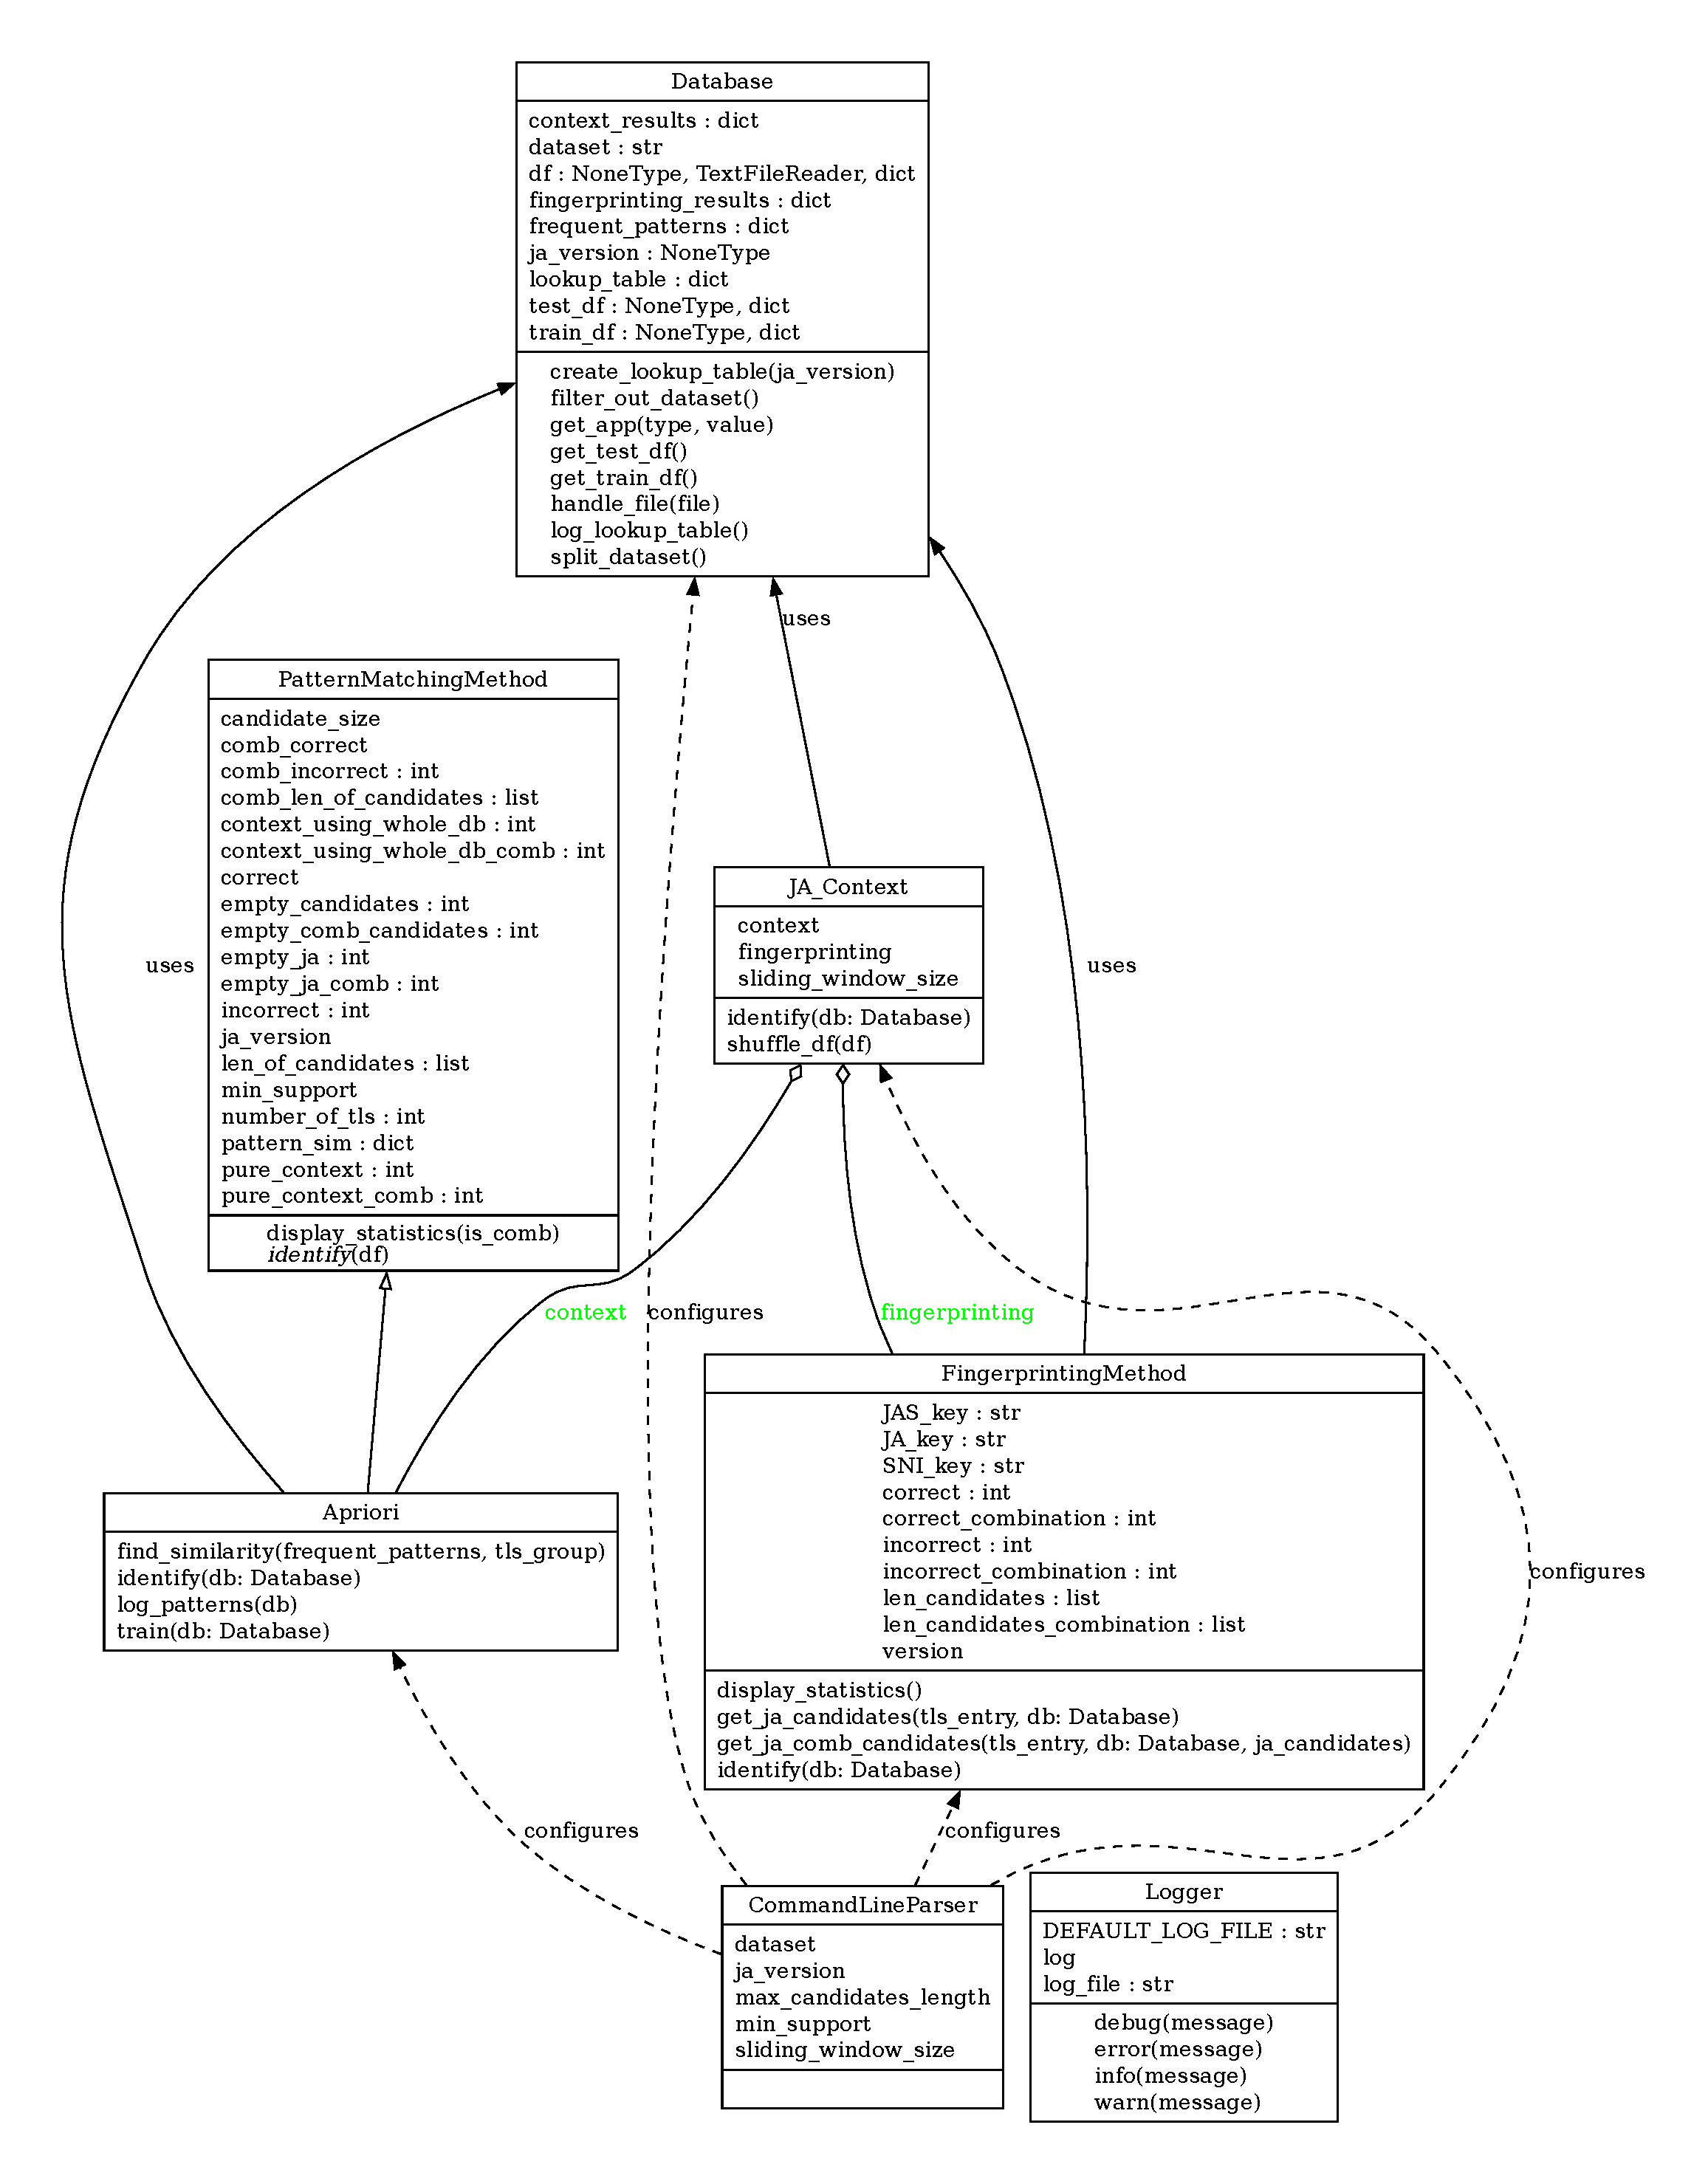
\includegraphics[width=0.7\textwidth]{obrazky-figures/class-dia-generated.pdf}
    \caption{Rozšířený diagram tříd}
    \label{fig:appendix-class}
\end{figure}

\chapter{Rozšířené výsledky experimentů}
\label{chp:appendix-experiments}
Tato kapitola obsahuje podrobné výstupy z~provedených experimentů. Jsou zde uvedeny grafy, tabulky a~další doplňující materiály, sloužící k~hlubší analýze a~interpretaci dosažených výsledků.

\section{Experiment 1}
\label{sec:appendix:ex1}

Následují neupravené a~nezkrácené tabulky uvádějící přesnost, průměrnou délku a~čas potřebný k~identifikaci pro~všechny testované kombinace.

\begin{table}[H]
    \centering
	\begin{tabular}{lrrrrr}
		\toprule
        \multicolumn{6}{c}{\textbf{Zúžení databáze kandidátů pomocí JA3}} \\
        \midrule
		\multirow{2}*{\textbf{Kombinace položek}}&\multicolumn{2}{c}{\texttt{iscx.csv}} & \multicolumn{3}{c}{\texttt{mobile\_desktop\_apps\_raw.csv}} \\
		                  & \textbf{Přesnost} & \textbf{Délka} & \textbf{Přesnost} & \textbf{Délka} & \textbf{Čas[s]} \\
		\midrule
		JA3               & 0.837              & 2.128           & 0.279              & 2.778           & 74.470        \\
		JA4               & 0.837              & 2.128           & 0.390              & 2.792           & 60.340        \\
		JA3+JA4           & 0.837              & 2.128           & 0.298              & 2.796           & 98.680        \\
		JA3+JA3S          & 0.847              & 2.128           & 0.365              & 2.796           & 101.050       \\
		JA4+JA4S          & 0.842              & 2.128           & 0.487              & 2.796           & 112.910       \\
		JA3+JA3S+SNI      & 0.852              & 2.128           & 0.371              & 2.796           & 163.680       \\
		JA4+JA4S+SNI      & 0.847              & 2.128           & 0.490              & 2.796           & 185.050       \\
		JA34S*            & 0.842              & 2.128           & 0.444              & 2.796           & 363.750       \\
		JA34S*+SNI        & 0.842              & 2.128           & 0.441              & 2.796           & 575.500       \\
		JA34S*+SNI+ORG    & 0.849              & 2.128           & 0.423              & 2.796           & 1123.730      \\
		JA34S*+SNI+ORG+CE & 0.849              & 2.128           & 0.379              & 2.796           & 2157.100      \\
		
		\bottomrule
	\end{tabular}
	\caption{Výsledky experimentu s~kombinacemi položek při~zúžení databáze kandidátů pomocí otisku \textit{JA3}}
	\label{tab:appendix-merged-not_comb-accuracy-ja3}
\end{table}

\begin{table}[H]
    \centering
	\begin{tabular}{lrrrrr}
		\toprule
        \multicolumn{6}{c}{\textbf{Zúžení databáze kandidátů pomocí JA4}} \\
        \midrule
		\multirow{2}*{\textbf{Kombinace položek}}&\multicolumn{2}{c}{\texttt{iscx.csv}} & \multicolumn{3}{c}{\texttt{mobile\_desktop\_apps\_raw.csv}} \\
		                  & \textbf{Přesnost} & \textbf{Délka} & \textbf{Přesnost} & \textbf{Délka} & \textbf{Čas[s]} \\
		\midrule
		JA3               & 0.837              & 2.128           & 0.304              & 2.781           & 53.660        \\
		JA4               & 0.837              & 2.128           & 0.387              & 2.785           & 32.340        \\
		JA3+JA4           & 0.837              & 2.128           & 0.361              & 2.789           & 48.100        \\
		JA3+JA3S          & 0.847              & 2.128           & 0.507              & 2.791           & 46.220        \\
		JA4+JA4S          & 0.842              & 2.128           & 0.558              & 2.791           & 58.500        \\
		JA3+JA3S+SNI      & 0.852              & 2.128           & 0.489              & 2.791           & 66.340        \\
		JA4+JA4S+SNI      & 0.847              & 2.128           & 0.548              & 2.791           & 84.030        \\
		JA34S*            & 0.842              & 2.128           & 0.577              & 2.791           & 150.820       \\
		JA34S*+SNI        & 0.842              & 2.128           & 0.549              & 2.791           & 225.220       \\
		JA34S*+SNI+ORG    & 0.849              & 2.128           & 0.533              & 2.791           & 400.770       \\
		JA34S*+SNI+ORG+CE & 0.849              & 2.128           & 0.507              & 2.791           & 840.660       \\
		
		\bottomrule
	\end{tabular}
	\caption{Výsledky experimentu s~kombinacemi položek při~zúžení databáze kandidátů pomocí otisku \textit{JA4}}
	\label{tab:appendix-merged-not_comb-accuracy-ja4}
\end{table}

\begin{table}[H]
    \centering
	\begin{tabular}{lrrrrr}
		\toprule
        \multicolumn{6}{c}{\textbf{Zúžení databáze kandidátů pomocí JA3+JA3S+SNI}} \\
        \midrule
		\multirow{2}*{\textbf{Kombinace položek}}&\multicolumn{2}{c}{\texttt{iscx.csv}} & \multicolumn{3}{c}{\texttt{mobile\_desktop\_apps\_raw.csv}} \\
		                  & \textbf{Přesnost} & \textbf{Délka} & \textbf{Přesnost} & \textbf{Délka} & \textbf{Čas[s]} \\
		\midrule
		JA3               & 0.867              & 1.583           & 0.385              & 2.287           & 74.470        \\
		JA4               & 0.867              & 1.583           & 0.771              & 1.747           & 60.340        \\
		JA3+JA4           & 0.872              & 1.583           & 0.764              & 1.745           & 98.680        \\
		JA3+JA3S          & 0.872              & 1.583           & 0.793              & 1.734           & 101.050       \\
		JA4+JA4S          & 0.869              & 1.583           & 0.800              & 1.734           & 112.910       \\
		JA3+JA3S+SNI      & 0.872              & 1.583           & 0.790              & 1.734           & 163.680       \\
		JA4+JA4S+SNI      & 0.867              & 1.583           & 0.798              & 1.734           & 185.050       \\
		JA34S*            & 0.867              & 1.583           & 0.793              & 1.734           & 363.750       \\
		JA34S*+SNI        & 0.867              & 1.583           & 0.792              & 1.734           & 575.500       \\
		JA34S*+SNI+ORG    & 0.869              & 1.583           & 0.774              & 1.734           & 1123.730      \\
		JA34S*+SNI+ORG+CE & 0.869              & 1.583           & 0.761              & 1.734           & 2157.100      \\
		
		\bottomrule
	\end{tabular}
	\caption{Výsledky experimentu s~kombinacemi položek při~zúžení databáze kandidátů pomocí kombinace  \textit{JA3+JA3S+SNI}}
	\label{tab:appendix-merged-comb-accuracy-ja3}
\end{table}


\begin{table}[H]
    \centering
	\begin{tabular}{lrrrrr}
		\toprule
        \multicolumn{6}{c}{\textbf{Zúžení databáze kandidátů pomocí JA4+JA4S+SNI}} \\
        \midrule
		\multirow{2}*{\textbf{Kombinace položek}}&\multicolumn{2}{c}{\texttt{iscx.csv}} & \multicolumn{3}{c}{\texttt{mobile\_desktop\_apps\_raw.csv}} \\
		                  & \textbf{Přesnost} & \textbf{Délka} & \textbf{Přesnost} & \textbf{Délka} & \textbf{Čas[s]} \\
		\midrule
		JA3               & 0.869              & 1.585           & 0.385              & 2.277           & 53.660        \\
		JA4               & 0.869              & 1.585           & 0.770              & 1.727           & 32.340        \\
		JA3+JA4           & 0.869              & 1.585           & 0.768              & 1.726           & 48.100        \\
		JA3+JA3S          & 0.874              & 1.585           & 0.793              & 1.714           & 46.220        \\
		JA4+JA4S          & 0.869              & 1.585           & 0.798              & 1.714           & 58.500        \\
		JA3+JA3S+SNI      & 0.874              & 1.585           & 0.795              & 1.714           & 66.340        \\
		JA4+JA4S+SNI      & 0.869              & 1.585           & 0.804              & 1.714           & 84.030        \\
		JA34S*            & 0.869              & 1.585           & 0.795              & 1.714           & 150.820       \\
		JA34S*+SNI        & 0.869              & 1.585           & 0.797              & 1.714           & 225.220       \\
		JA34S*+SNI+ORG    & 0.872              & 1.585           & 0.782              & 1.714           & 400.770       \\
		JA34S*+SNI+ORG+CE & 0.872              & 1.585           & 0.774              & 1.714           & 840.660       \\
		
		\bottomrule
	\end{tabular}
	\caption{Výsledky experimentu s~kombinacemi položek při~zúžení databáze kandidátů pomocí kombinace  \textit{JA4+JA4S+SNI}}
	\label{tab:appendix-merged-comb-accuracy-ja4}
\end{table}

\section{Experiment 2}
\label{sec:appendix:ex2}

Zde jsou uvedeny heatmapy znázorňující výsledky při~použití otisků \texttt{JA4} jako základní metody pro~generování počáteční kandidátní množiny.

\begin{figure}[H]
    \centering
    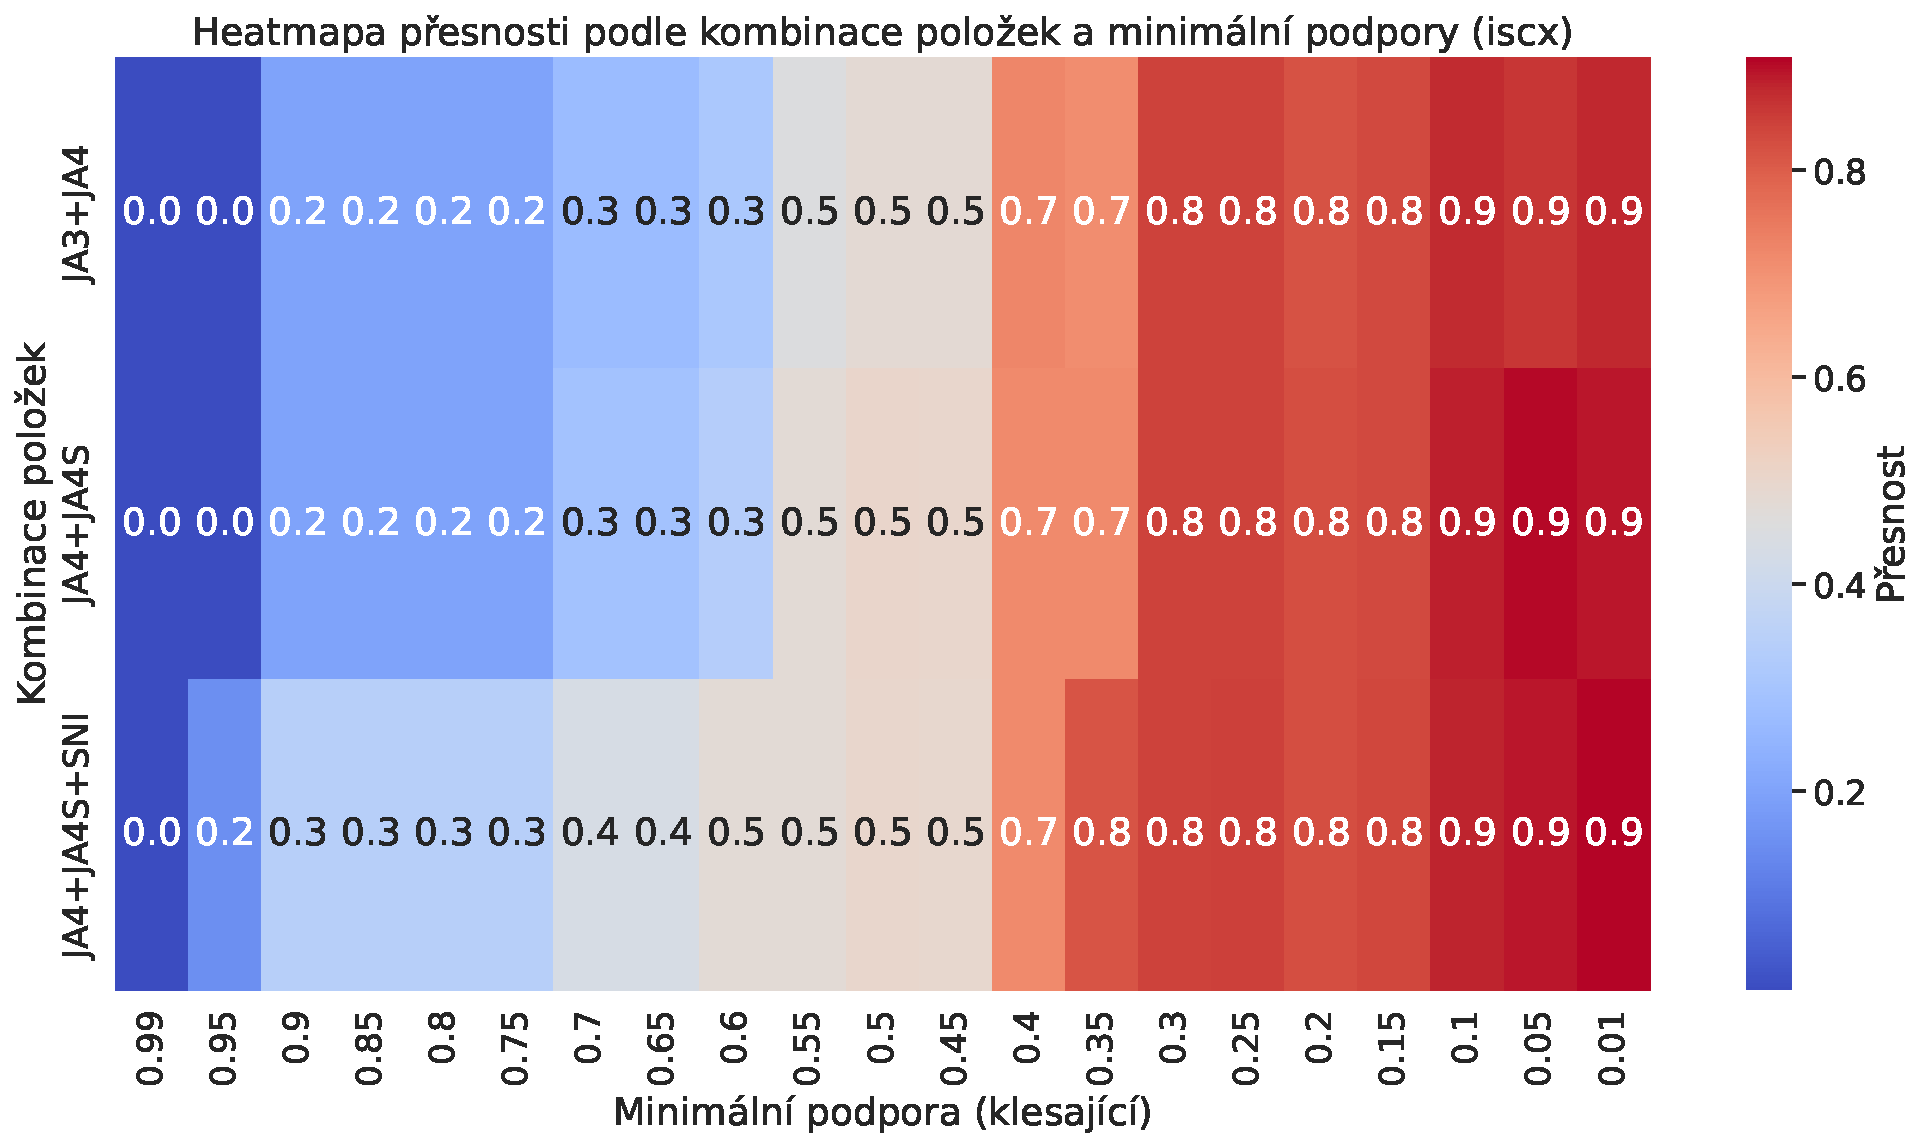
\includegraphics[width=\linewidth]{obrazky-figures/exps/ex2-iscx-heatmap_not_comb.pdf}
    \caption{Heatmapa zobrazující testované kombinace položek v~závislosti na~volbě minimální podpory a~dosažené přesnosti pro~datovou sadu \texttt{iscx.csv} při~použití otisků \textit{JA4}. }
    \label{fig:appendix-heatmap-iscx}
\end{figure}

\begin{figure}[H]
    \centering
    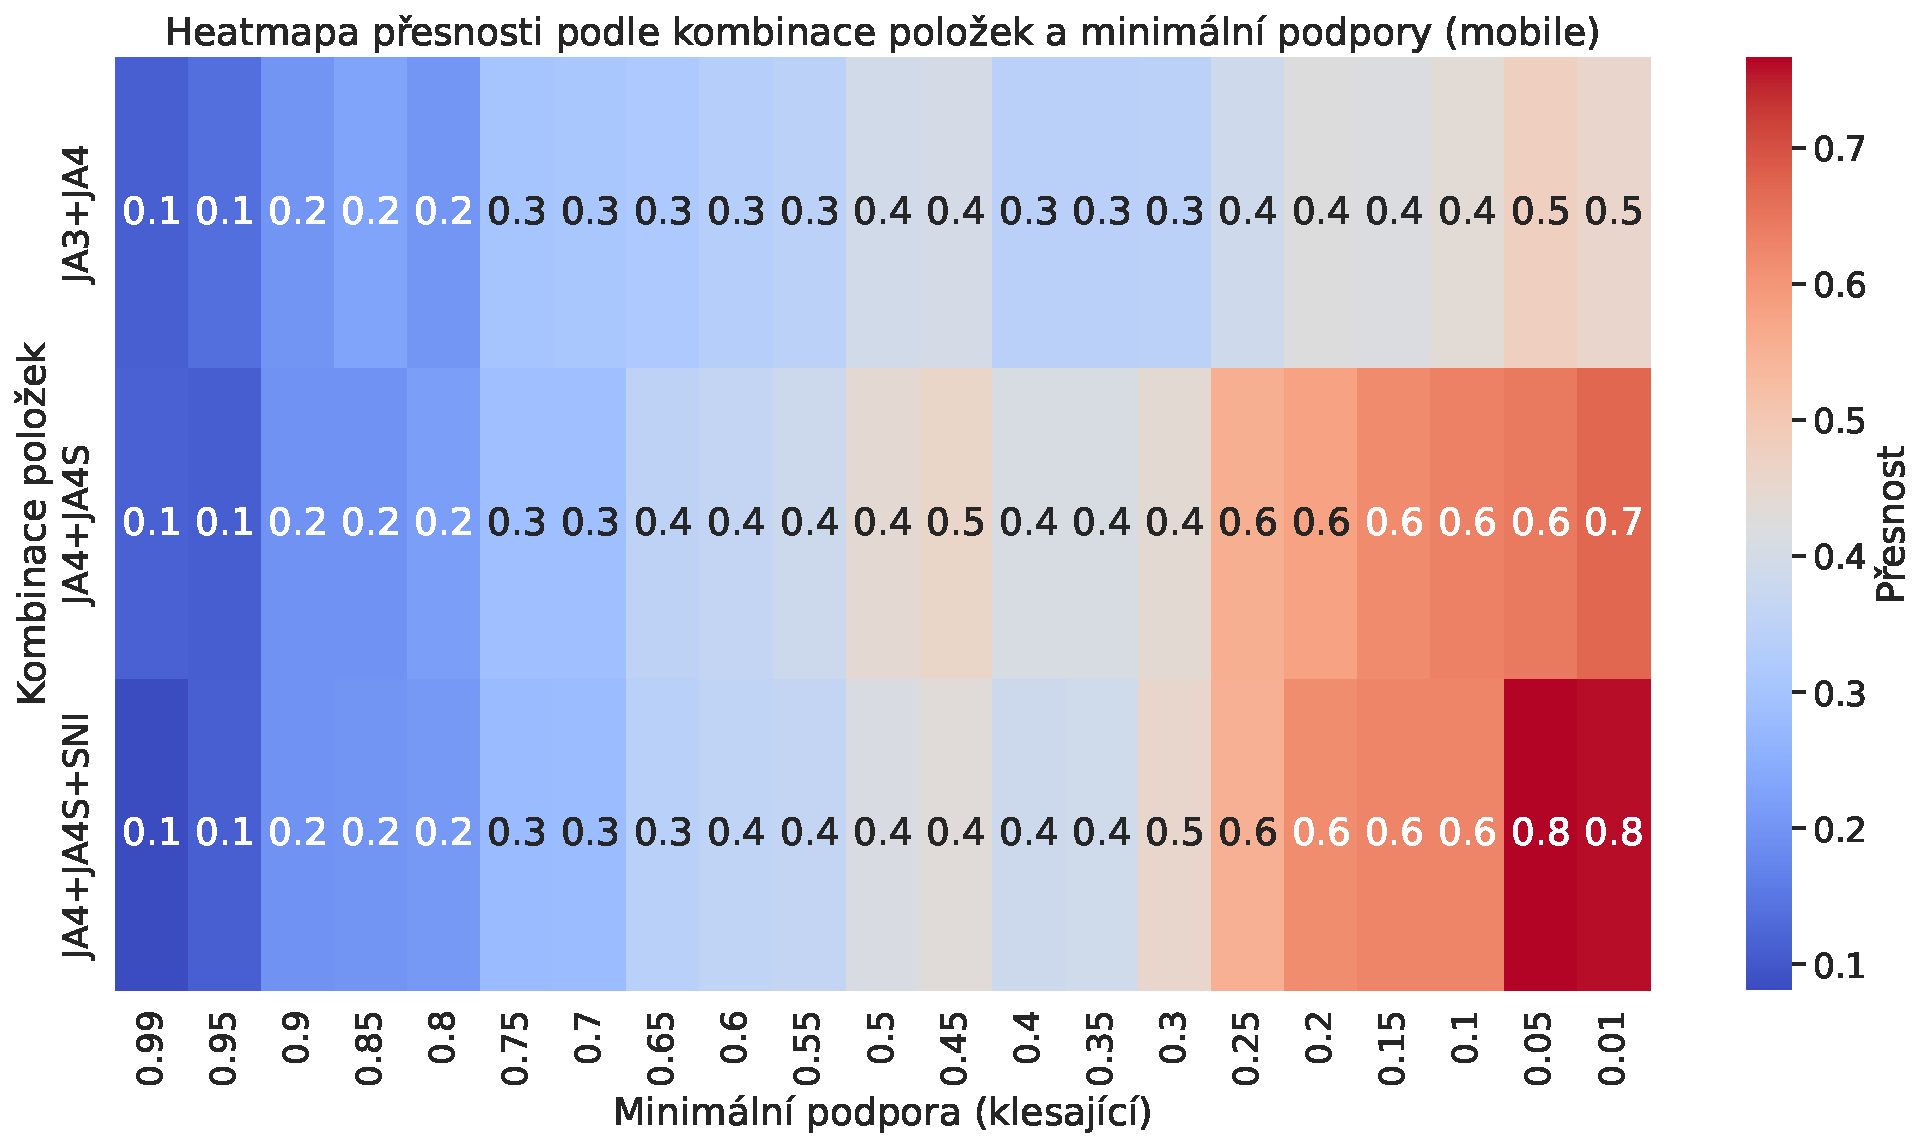
\includegraphics[width=\linewidth]{obrazky-figures/exps/ex2-mobile-heatmap_not_comb.pdf}
    \caption{Heatmapa zobrazující testované kombinace položek v~závislosti na~volbě minimální podpory a~dosažené přesnosti pro~datovou sadu \texttt{mobile desktop apps raw.csv} při~použití otisků \textit{JA4}. }
    \label{fig:appendix-heatmap-mobile}
\end{figure}

\begin{figure}[H]
    \centering
    \begin{minipage}[t]{0.49\textwidth}
        \centering
    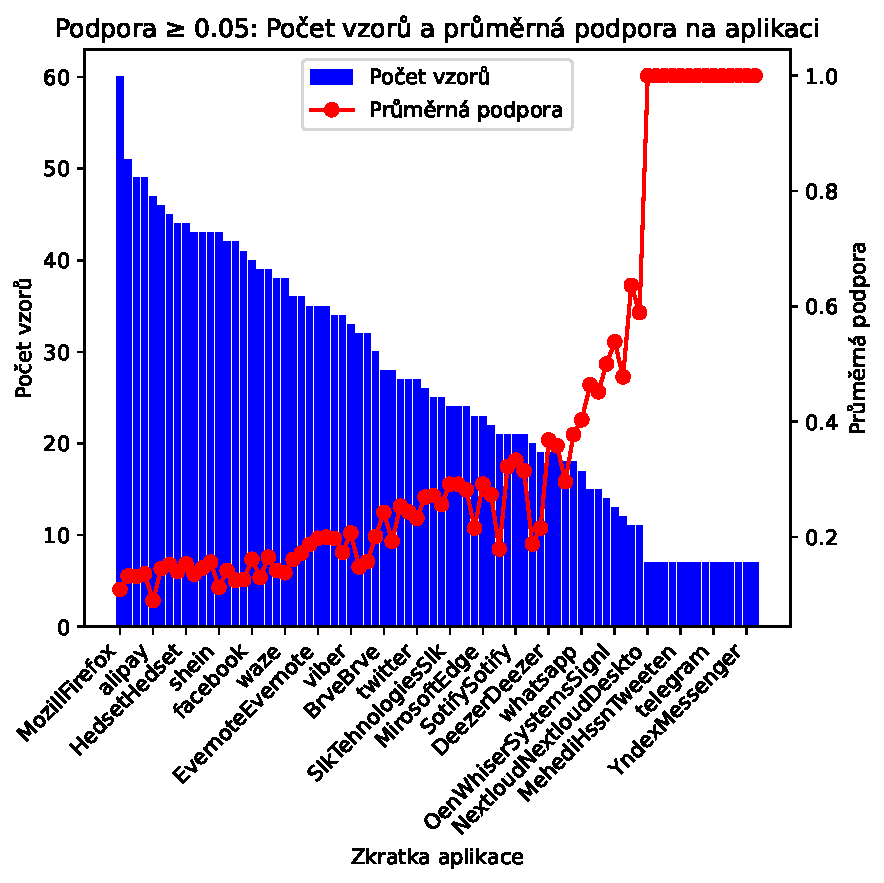
\includegraphics[width=\linewidth]{obrazky-figures/exps/patterns_support_0.05_mobile.pdf}
    \caption{Počet vzorů a~průměrná podpora na~aplikaci pro~\texttt{mobile desktop apps raw.csv} při~minimální podpoře 0.05.}
    \label{fig:appendix-}
    \end{minipage}%
    \hfill
    \begin{minipage}[t]{0.49\textwidth}
       \centering
        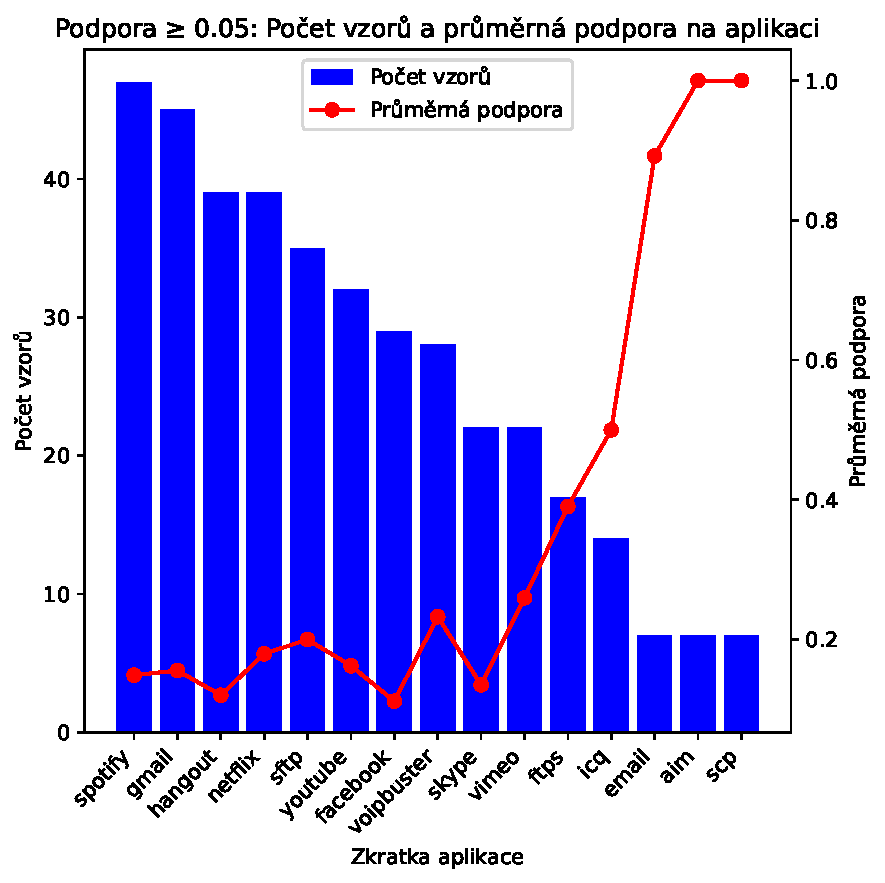
\includegraphics[width=\linewidth]{obrazky-figures/exps/patterns_support_0.05_iscx.pdf}
        \caption{Počet vzorů a~průměrná podpora na~aplikaci pro~\texttt{iscx.csv} při~minimální podpoře 0.05.}
        \label{fig:appendix-}
    \end{minipage}
\end{figure}

\begin{figure}[H]
    \centering
    \begin{minipage}[t]{0.49\textwidth}
        \centering
    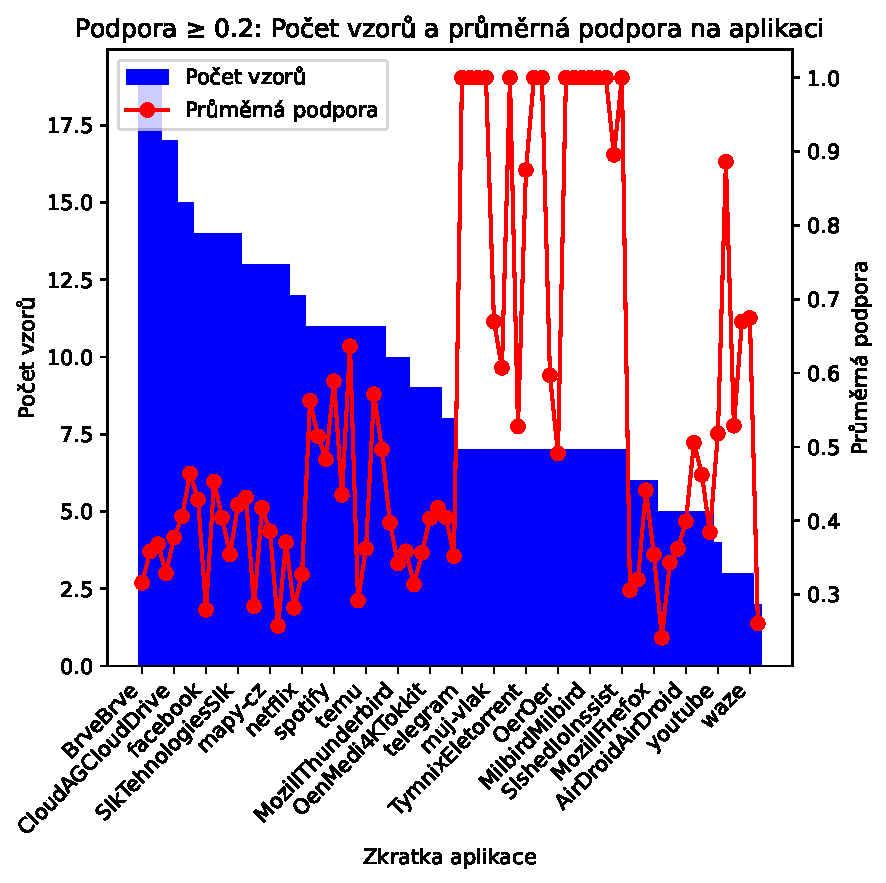
\includegraphics[width=\linewidth]{obrazky-figures/exps/patterns_support_0.2_mobile.pdf}
    \caption{Počet vzorů a~průměrná podpora na~aplikaci pro~\texttt{mobile desktop apps raw.csv} při~minimální podpoře 0.2.}
    \label{fig:appendix-}
    \end{minipage}%
    \hfill
    \begin{minipage}[t]{0.49\textwidth}
       \centering
        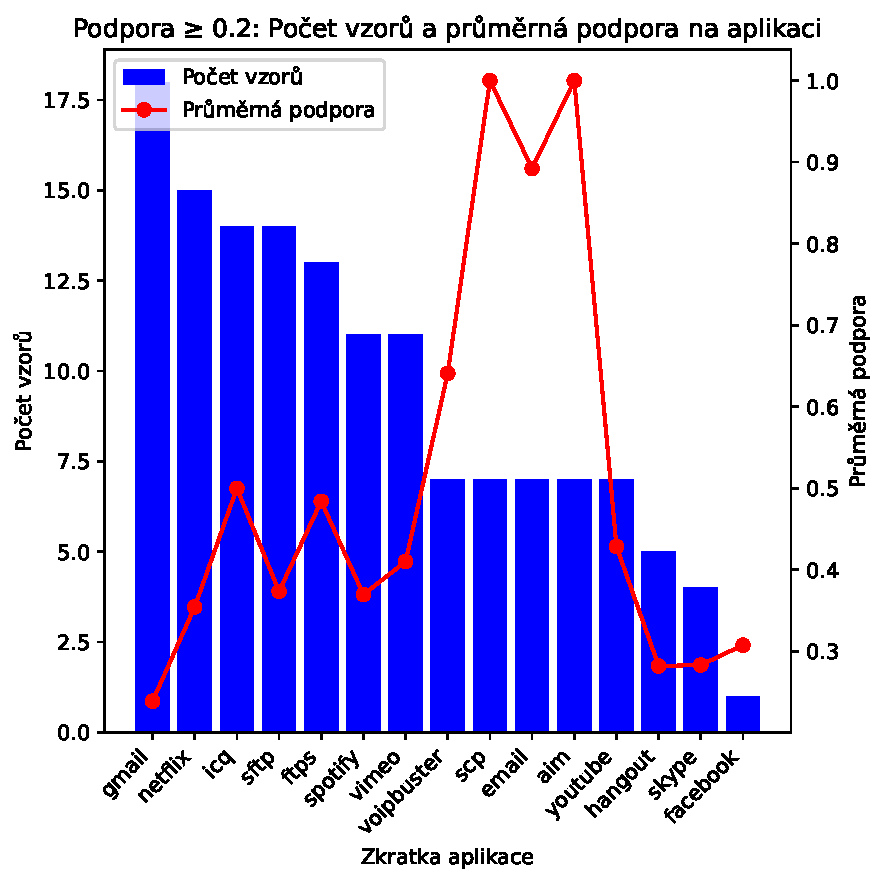
\includegraphics[width=\linewidth]{obrazky-figures/exps/patterns_support_0.2_iscx.pdf}
        \caption{Počet vzorů a~průměrná podpora na~aplikaci pro~\texttt{iscx.csv} při~minimální podpoře 0.2.}
        \label{fig:appendix-}
    \end{minipage}
\end{figure}

\begin{figure}[H]
    \centering
    \begin{minipage}[t]{0.49\textwidth}
        \centering
    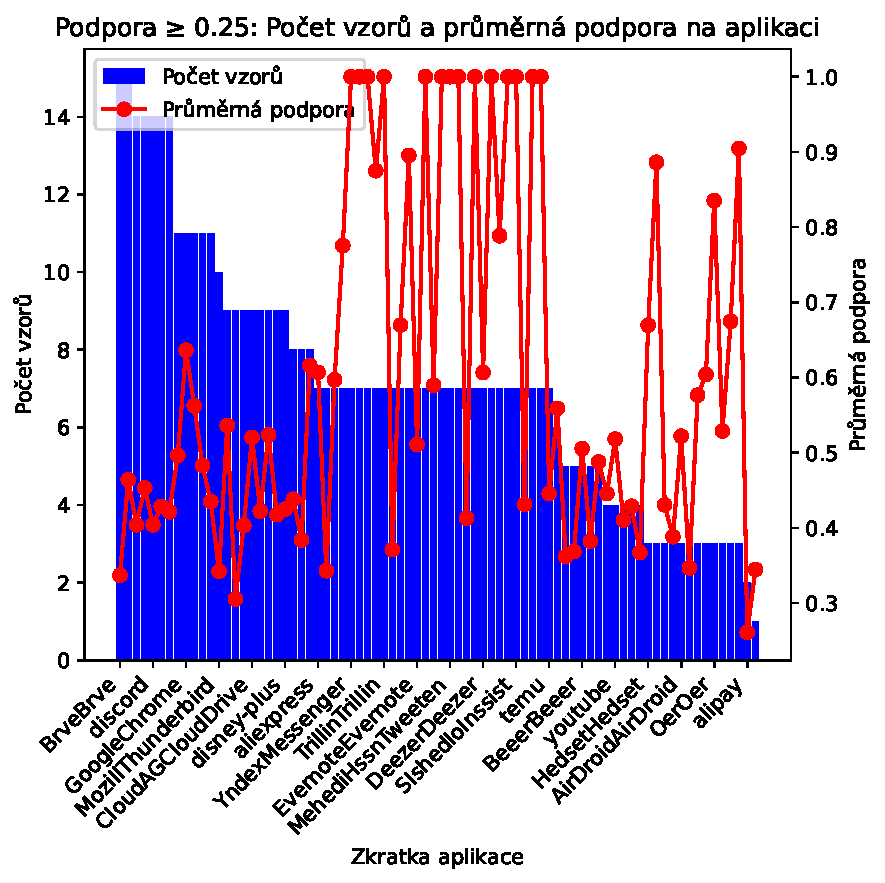
\includegraphics[width=\linewidth]{obrazky-figures/exps/patterns_support_0.25_mobile.pdf}
    \caption{Počet vzorů a~průměrná podpora na~aplikaci pro~\texttt{mobile desktop apps raw.csv} při~minimální podpoře 0.25.}
    \label{fig:appendix-}
    \end{minipage}%
    \hfill
    \begin{minipage}[t]{0.49\textwidth}
       \centering
        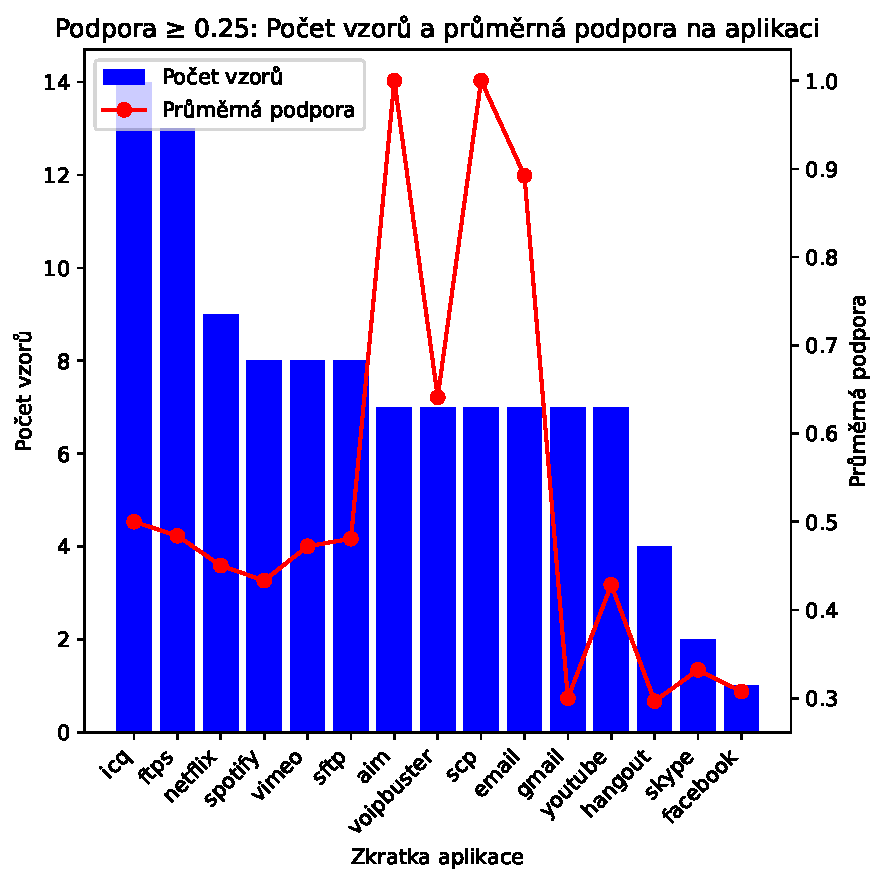
\includegraphics[width=\linewidth]{obrazky-figures/exps/patterns_support_0.25_iscx.pdf}
        \caption{Počet vzorů a~průměrná podpora na~aplikaci pro~\texttt{iscx.csv} při~minimální podpoře 0.25.}
        \label{fig:appendix-}
    \end{minipage}
\end{figure}

\begin{figure}[H]
    \centering
    \begin{minipage}[t]{0.49\textwidth}
        \centering
    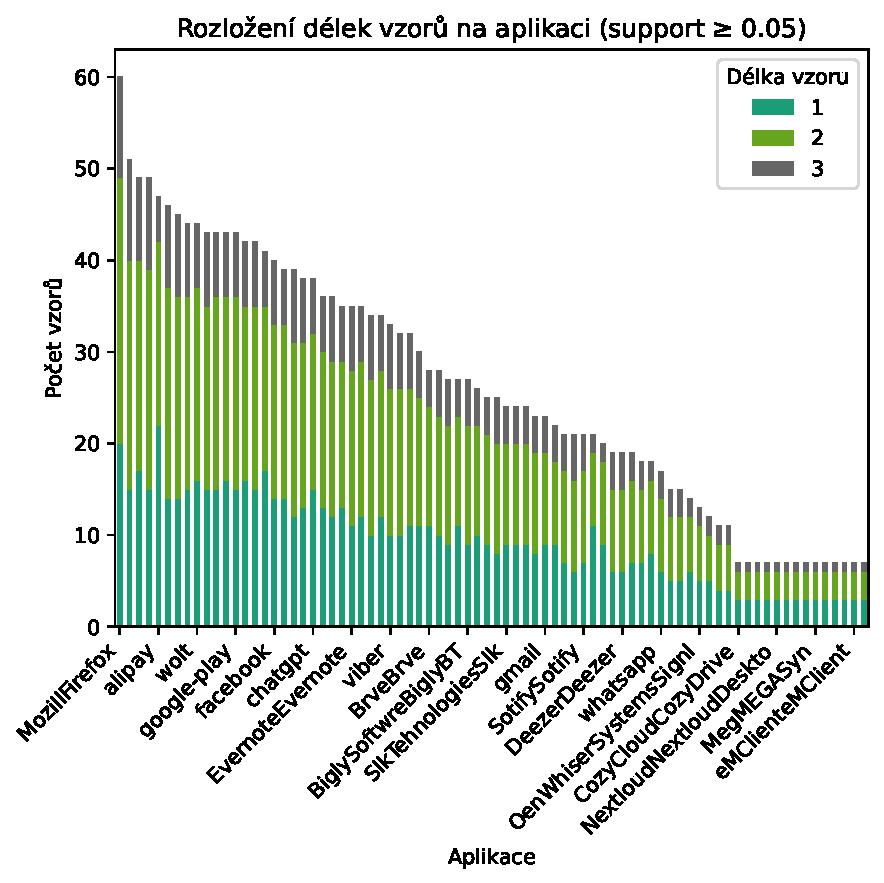
\includegraphics[width=\linewidth]{obrazky-figures/exps/pattern_lengths_0.05_mobile.pdf}
        \caption{Počet vzorů a~rozložení délek vzoru na~aplikaci pro~\texttt{mobile desktop apps raw.csv} při~minimální podpoře 0.05.}
    \label{fig:appendix-}
    \end{minipage}%
    \hfill
    \begin{minipage}[t]{0.49\textwidth}
       \centering
        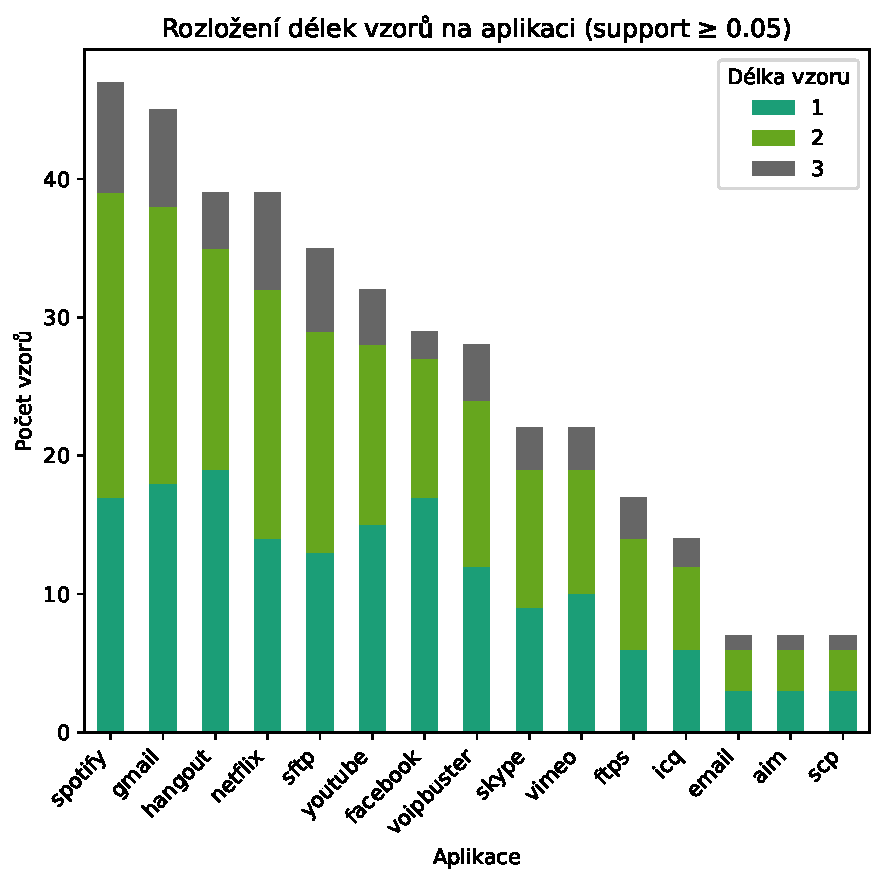
\includegraphics[width=\linewidth]{obrazky-figures/exps/pattern_lengths_0.05_iscx.pdf}

            \caption{Počet vzorů a~rozložení délek vzoru na~aplikaci pro~\texttt{iscx.csv} při~minimální podpoře 0.05.}
        \label{fig:appendix-}
    \end{minipage}
\end{figure}

\begin{figure}[H]
    \centering
    \begin{minipage}[t]{0.49\textwidth}
        \centering
    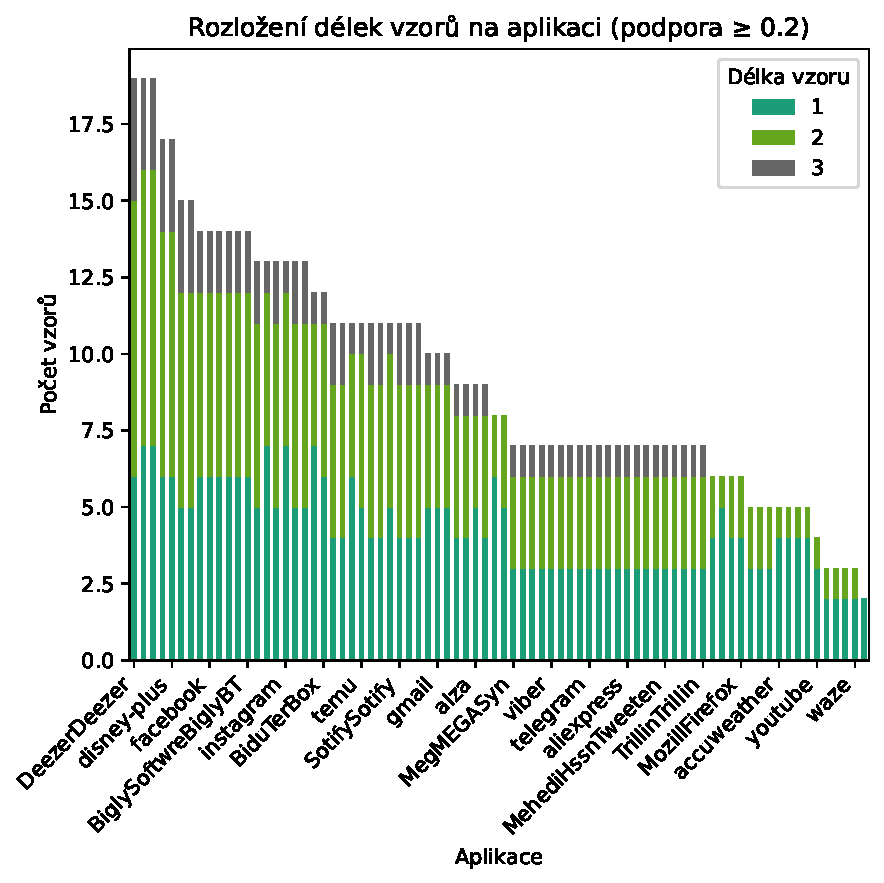
\includegraphics[width=\linewidth]{obrazky-figures/exps/pattern_lengths_0.2_mobile.pdf}
        \caption{Počet vzorů a~rozložení délek vzoru na~aplikaci pro~\texttt{mobile desktop apps raw.csv} při~minimální podpoře 0.2.}
    \label{fig:appendix-}
    \end{minipage}%
    \hfill
    \begin{minipage}[t]{0.49\textwidth}
       \centering
        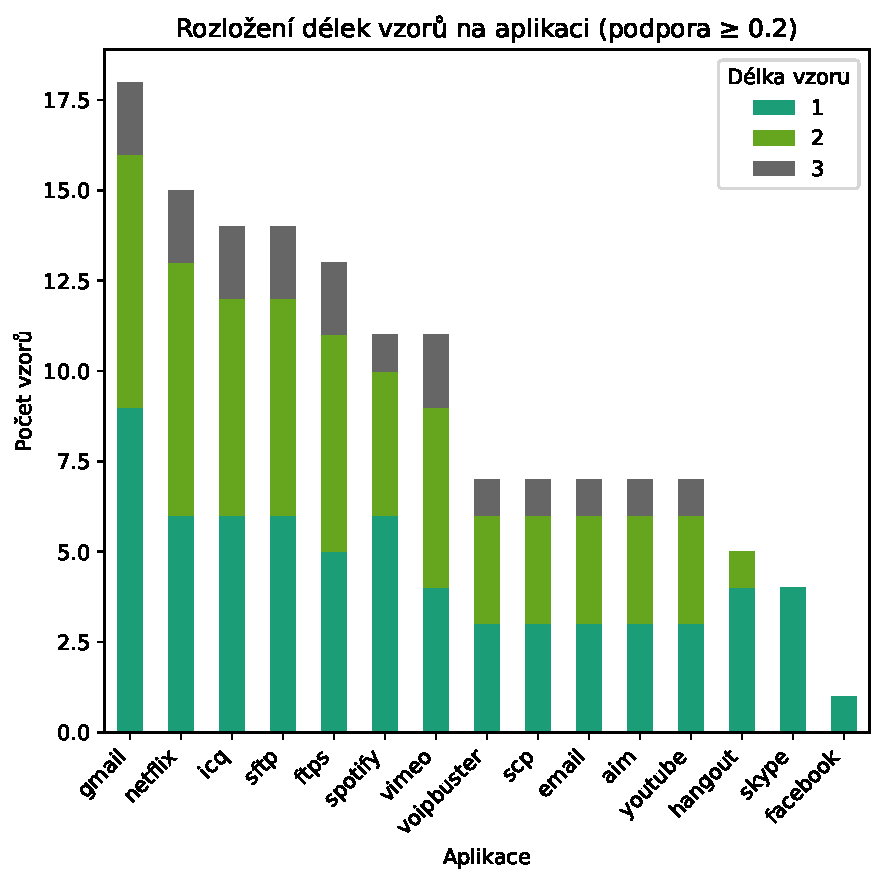
\includegraphics[width=\linewidth]{obrazky-figures/exps/pattern_lengths_0.2_iscx.pdf}

            \caption{Počet vzorů a~rozložení délek vzoru na~aplikaci pro~\texttt{iscx.csv} při~minimální podpoře 0.2.}
        \label{fig:appendix-}
    \end{minipage}
\end{figure}

\begin{figure}[H]
    \centering
     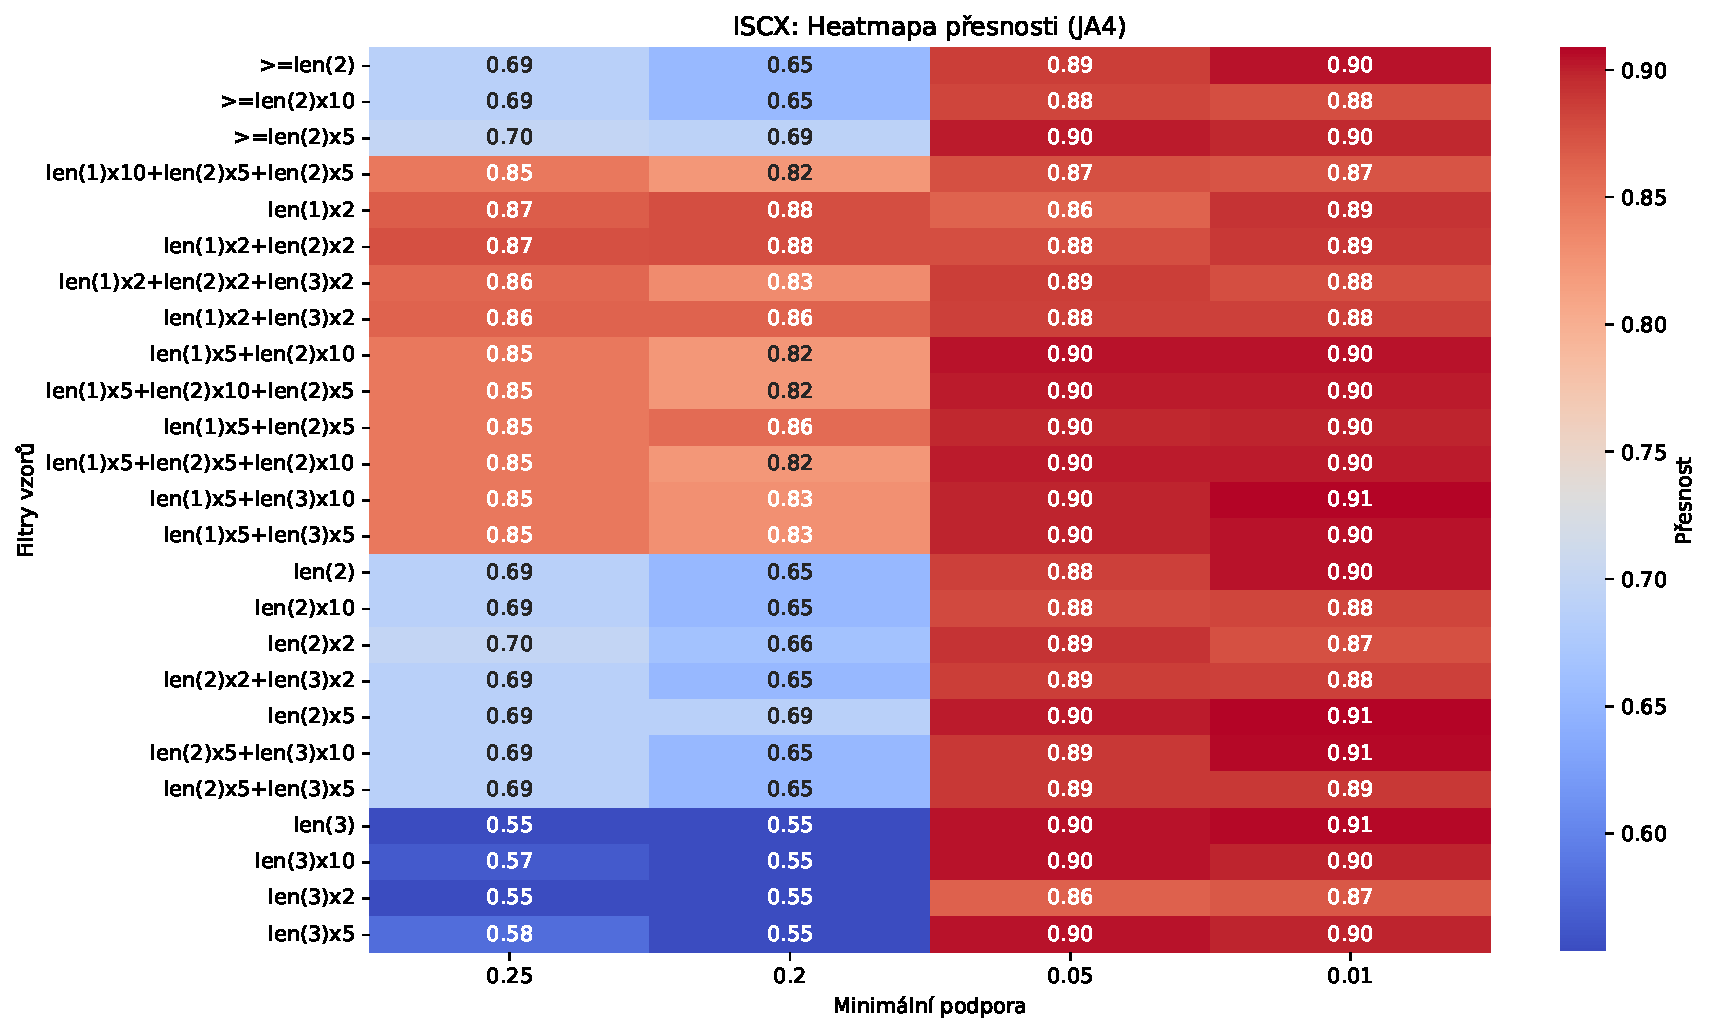
\includegraphics[angle=-90, width=0.8\textwidth]{obrazky-figures/exps/ex3-iscx-heatmap-JA4.pdf}
    \caption{Heatmapa zobrazuje testované kombinace otisků a~filtrů při~použití různých selekčních strategií nad~datovou sadou \texttt{iscx.csv}, konkrétně pro~kombinaci otisků \textit{JA4}. Barevné škálování reprezentuje dosaženou přesnost identifikace pro~každou konfiguraci.}
    \label{fig:appendix-heatmap-iscx-filter-ja4}
\end{figure}

\begin{figure}[H]
    \centering
    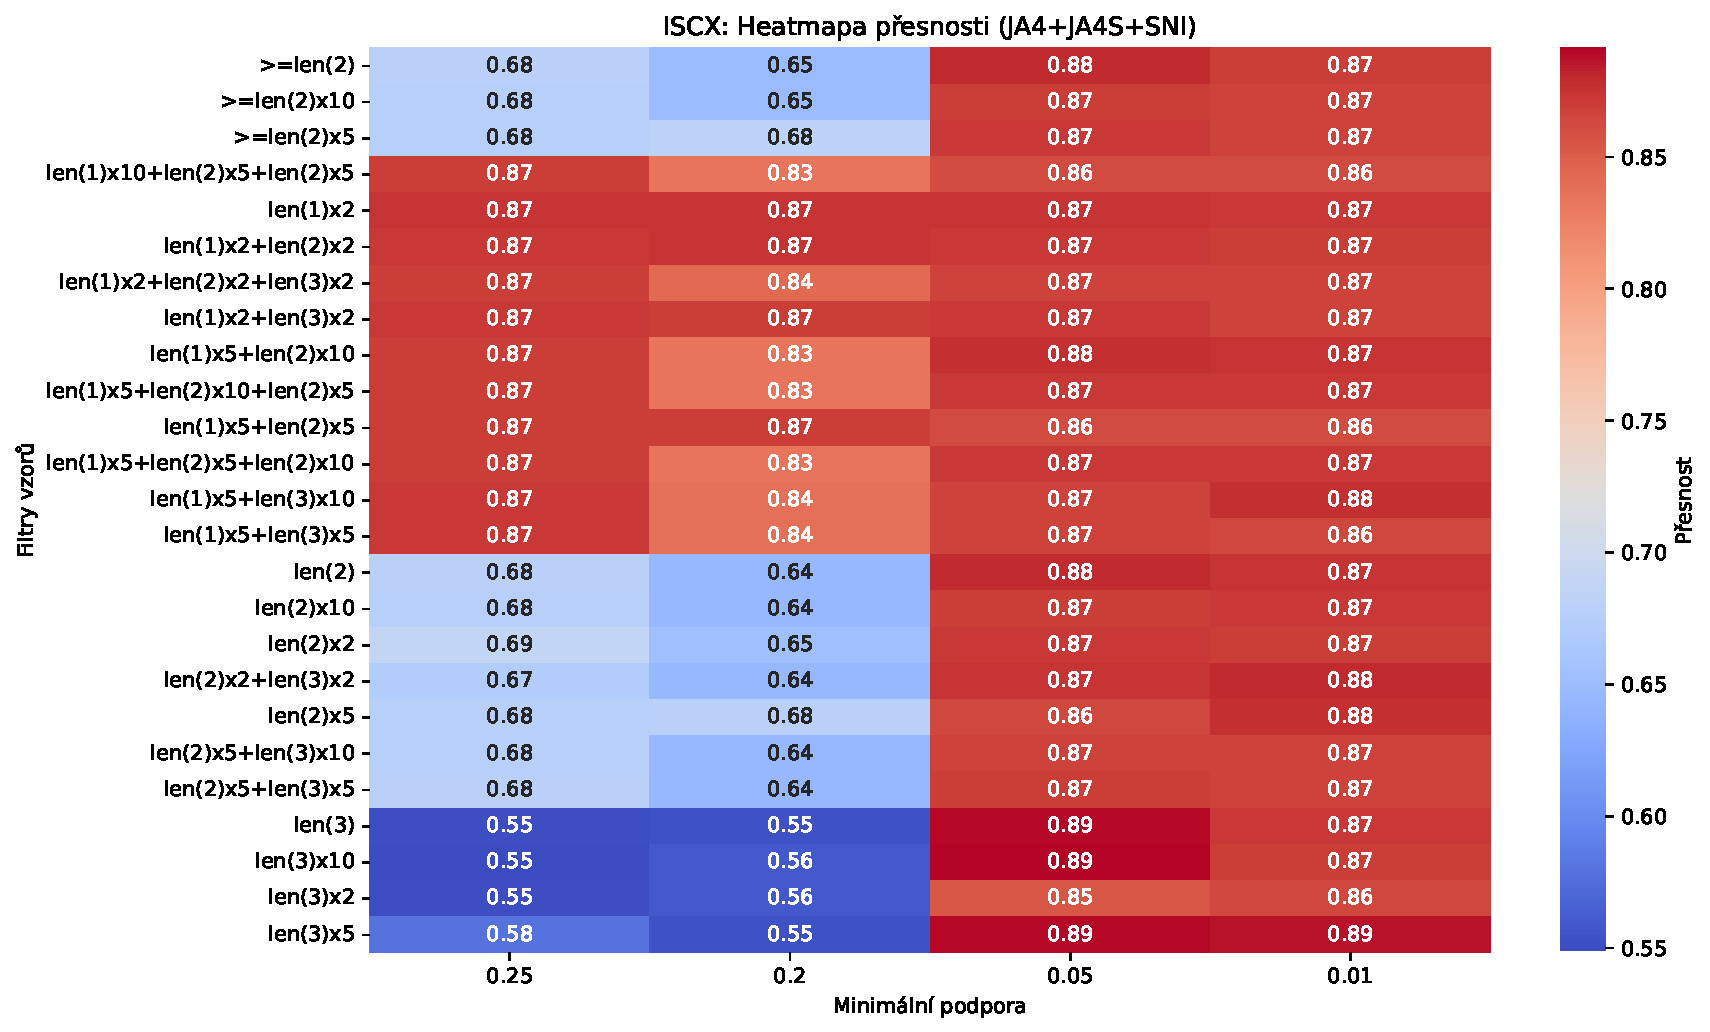
\includegraphics[angle=-90, width=0.8\textwidth]{obrazky-figures/exps/ex3-iscx-heatmap-JA4+JA4S+SNI.pdf}
    \caption{Heatmapa zobrazuje testované kombinace otisků a~filtrů při~použití různých selekčních strategií nad~datovou sadou \texttt{iscx.csv}, konkrétně pro~kombinaci otisků \textit{JA4+JA4S+SNI}. Barevné škálování reprezentuje dosaženou přesnost identifikace pro~každou konfiguraci.}
    \label{fig:appendix-heatmap-iscx-filter-ja4}
\end{figure}

\begin{figure}[H]
    \centering
    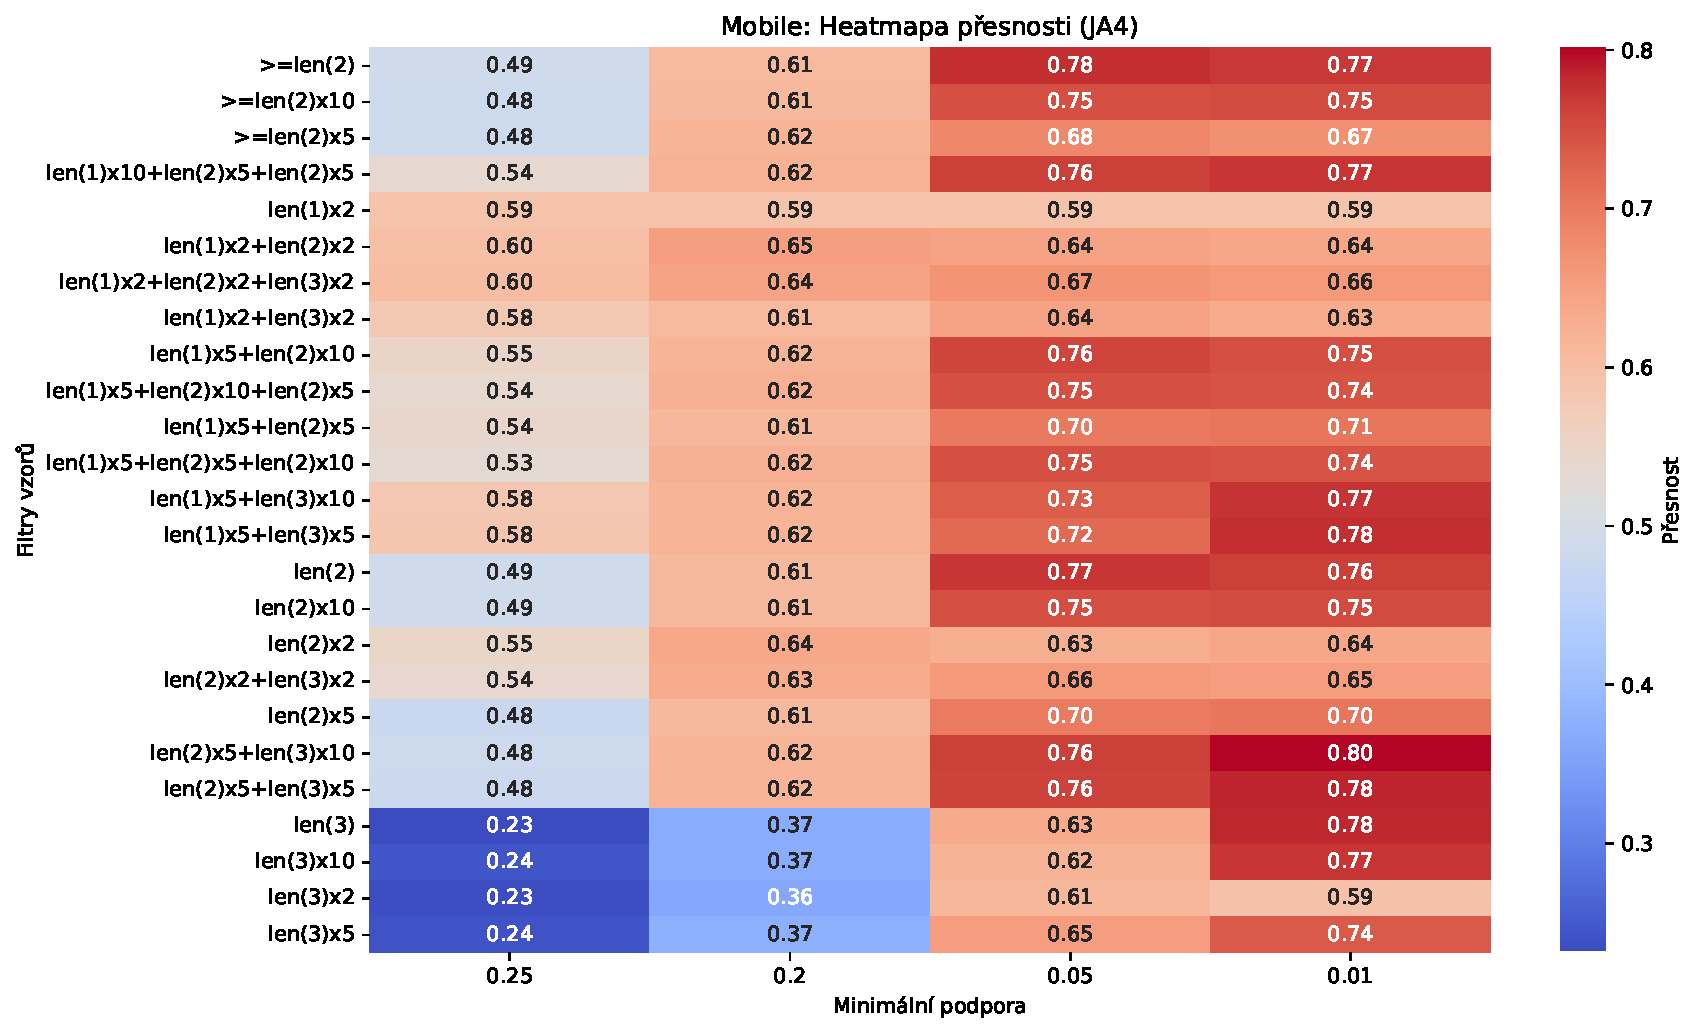
\includegraphics[angle=-90, width=0.8\textwidth]{obrazky-figures/exps/ex3-mobile-heatmap-JA4.pdf}
    \caption{Heatmapa zobrazuje testované kombinace otisků a~filtrů při~použití různých selekčních strategií nad~datovou sadou \texttt{mobile\_desktop\_apps\_raw.csv}, konkrétně pro~kombinaci otisků \textit{JA4}. Barevné škálování reprezentuje dosaženou přesnost identifikace pro~každou konfiguraci.}
    \label{fig:appendix-heatmap-iscx-filter-ja4}
\end{figure}

\begin{figure}[H]
    \centering
    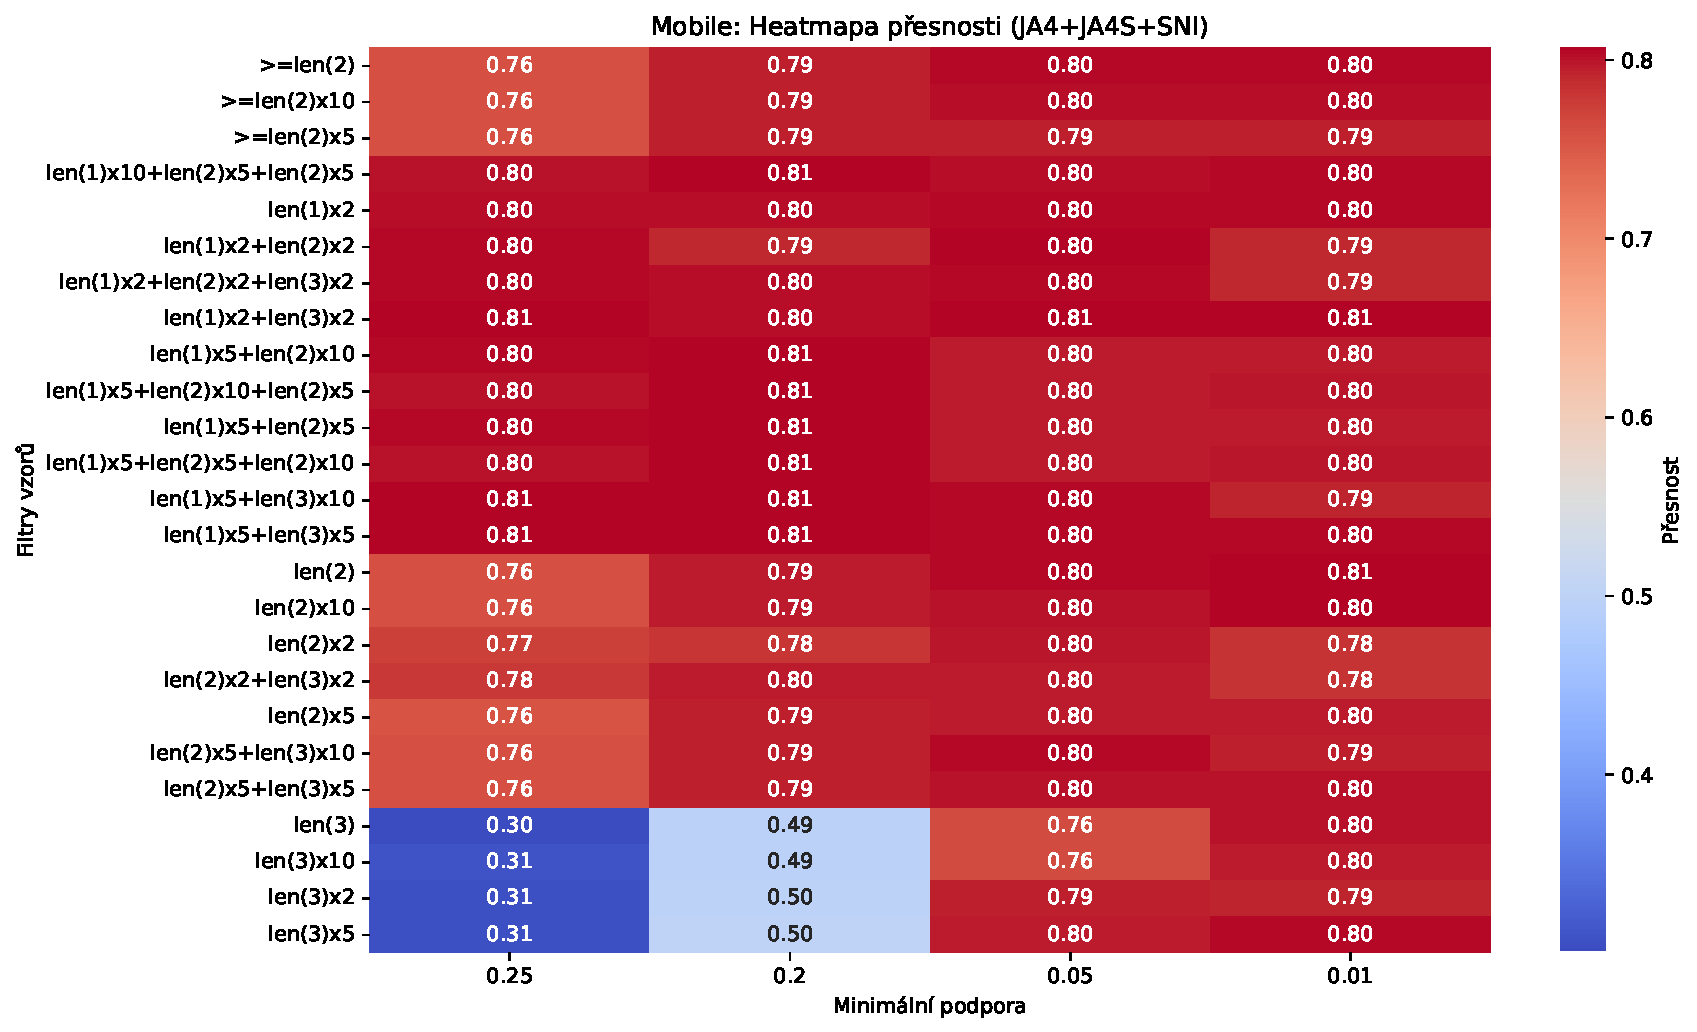
\includegraphics[angle=-90, width=0.8\textwidth]{obrazky-figures/exps/ex3-mobile-heatmap-JA4+JA4S+SNI.pdf}
    \caption{Heatmapa zobrazuje testované kombinace otisků a~filtrů při~použití různých selekčních strategií nad~datovou sadou \texttt{mobile\_desktop\_apps\_raw.csv}, konkrétně pro~kombinaci otisků \textit{JA4+JA4S+SNI}. Barevné škálování reprezentuje dosaženou přesnost identifikace pro~každou konfiguraci.}
    \label{fig:appendix-heatmap-iscx-filter-ja4}
\end{figure}

  \fi
  
  % Kompilace po částech (viz výše, nutno odkomentovat)
  % Compilation piecewise (see above, it is necessary to uncomment it)
  %\subfile{projekt-30-prilohy-appendices}

\end{document}
